%============================================================
%  ĐỒ ÁN TỐT NGHIỆP - ĐẠI HỌC BÁCH KHOA HÀ NỘI
%  Đề tài: Hệ thống AIoT giám sát và dự báo chất lượng
%          không khí dựa trên dữ liệu chuỗi thời gian
%============================================================

\documentclass[12pt, a4paper, oneside]{report}

%------------------------------------------------------------
% ENCODING & FONT
%------------------------------------------------------------
\usepackage[utf8]{inputenc}
\usepackage[T5]{fontenc}
\usepackage[vietnamese,english]{babel}
\usepackage{times}

%------------------------------------------------------------
% PAGE LAYOUT
% Fix lỗi headheight quá nhỏ: tăng lên 15.5pt
%------------------------------------------------------------
\usepackage[
  top=30mm,
  bottom=25mm,
  left=35mm,
  right=20mm,
  headheight=15.5pt      % fix fancyhdr warning
]{geometry}

%------------------------------------------------------------
% SPACING & FORMATTING
%------------------------------------------------------------
\usepackage{setspace}
\onehalfspacing
\usepackage{indentfirst}
\setlength{\parindent}{1.27cm}
\setlength{\parskip}{6pt}

%------------------------------------------------------------
% HEADERS & FOOTERS
%------------------------------------------------------------
\usepackage{fancyhdr}
\pagestyle{fancy}
\fancyhf{}
\fancyhead[R]{\small\leftmark}
\fancyfoot[C]{\thepage}
\renewcommand{\headrulewidth}{0.4pt}
\fancypagestyle{plain}{
  \fancyhf{}
  \fancyfoot[C]{\thepage}
  \renewcommand{\headrulewidth}{0pt}
}

%------------------------------------------------------------
% GRAPHICS & FIGURES
%------------------------------------------------------------
\usepackage{graphicx}
\usepackage{float}
\graphicspath{{images/}}

%------------------------------------------------------------
% TABLES
%------------------------------------------------------------
\usepackage{booktabs}
\usepackage{longtable}
\usepackage{multirow}
\usepackage{array}
\usepackage{tabularx}

%------------------------------------------------------------
% MATH
%------------------------------------------------------------
\usepackage{amsmath, amssymb}

%------------------------------------------------------------
% CODE LISTINGS
%------------------------------------------------------------
\usepackage{xcolor}
\usepackage{listings}
\lstdefinelanguage{JavaScript}{
  keywords={async,await,break,case,catch,const,continue,default,else,for,function,if,let,module,require,return,switch,throw,try,var,while},
  sensitive=true,
  comment=[l]{//},
  morecomment=[s]{/*}{*/},
  morestring=[b]',
  morestring=[b]",
  morestring=[b]`
}
\lstset{
  basicstyle=\small\ttfamily,
  keywordstyle=\bfseries\color{blue!70!black},
  commentstyle=\itshape\color{gray},
  stringstyle=\color{red!60!black},
  numbers=left,
  numberstyle=\tiny\color{gray},
  stepnumber=1,
  frame=single,
  breaklines=true,
  breakatwhitespace=false,
  captionpos=b,
  tabsize=2,
  showstringspaces=false
}

%------------------------------------------------------------
% HYPERLINKS
%------------------------------------------------------------
\usepackage[
  colorlinks=true,
  linkcolor=black,
  citecolor=black,
  urlcolor=blue,
  unicode=true
]{hyperref}

%------------------------------------------------------------
% BIBLIOGRAPHY
% Đổi từ biblatex+biber → natbib+bibtex: nhẹ hơn nhiều,
% không bị timeout trên Overleaf free plan
%------------------------------------------------------------
\usepackage[numbers, sort&compress]{natbib}

%------------------------------------------------------------
% CAPTIONS
%------------------------------------------------------------
\usepackage{caption}
\usepackage{subcaption}
\captionsetup{
  labelfont=bf,
  skip=6pt,
  font=small
}

%------------------------------------------------------------
% MISCELLANEOUS
% Bỏ microtype: không tương thích tốt với T5/ptm,
% gây nhiều warning và làm chậm compile
%------------------------------------------------------------
\usepackage{enumitem}
\usepackage{emptypage}

%------------------------------------------------------------
% CHAPTER TITLE STYLE (căn giữa, in hoa, chuẩn HUST)
%------------------------------------------------------------
\usepackage{titlesec}
\titleformat{\chapter}[display]
  {\normalfont\large\bfseries\centering}
  {\MakeUppercase{\chaptertitlename}\ \thechapter.}
  {0pt}
  {\large\MakeUppercase}
\titlespacing*{\chapter}{0pt}{-20pt}{20pt}

\titleformat{\section}
  {\normalfont\normalsize\bfseries}{\thesection}{1em}{}
\titleformat{\subsection}
  {\normalfont\normalsize\bfseries}{\thesubsection}{1em}{}
\titleformat{\subsubsection}
  {\normalfont\normalsize\itshape}{\thesubsubsection}{1em}{}

%------------------------------------------------------------
% TOC DEPTH
%------------------------------------------------------------
\setcounter{tocdepth}{3}
\setcounter{secnumdepth}{3}

%============================================================
% BEGIN DOCUMENT
%============================================================
\begin{document}
\selectlanguage{vietnamese}

% BÌA NGOÀI
%============================================================
% BÌA NGOÀI
%============================================================
\begin{titlepage}
\begin{center}

{\large\bfseries ĐẠI HỌC BÁCH KHOA HÀ NỘI}

\vspace{0.8cm}
{\Large\bfseries ĐỒ ÁN TỐT NGHIỆP}

\vspace{1.5cm}
{\LARGE\bfseries
Hệ thống AIoT giám sát và dự báo\\[6pt]
chất lượng không khí dựa trên\\[6pt]
dữ liệu chuỗi thời gian
}

\vspace{1.8cm}
% Nếu có logo trường, bỏ comment dòng dưới:
% \includegraphics[width=3cm]{hust_logo.png}\\[1cm]

{\large\bfseries Nguyễn Lê Hà Sơn}\\[4pt]
{\normalsize son.nlh225157@sis.hust.edu.vn}

\vspace{1.2cm}
\begin{tabular}{ll}
\textbf{Chương trình đào tạo:} & Kỹ thuật máy tính \\[4pt]
\end{tabular}

\vspace{1.2cm}
\begin{tabular}{ll}
\textbf{Giảng viên hướng dẫn:} & TS. Đỗ Công Thuần\\[4pt]
\end{tabular}

\vspace{0.5cm}
\begin{tabular}{ll}
\textbf{Khoa:} & Kỹ thuật máy tính \\[4pt]
\textbf{Trường:} & Công nghệ Thông tin và Truyền thông \\
\end{tabular}

\vfill
{\large\bfseries HÀ NỘI, 6/2026}

\end{center}
\end{titlepage}


% BÌA TRONG (có chữ ký GVHD)
%============================================================
% BÌA TRONG (có ô chữ ký GVHD)
%============================================================
\begin{titlepage}
\begin{center}

{\large\bfseries ĐẠI HỌC BÁCH KHOA HÀ NỘI}

\vspace{0.8cm}
{\Large\bfseries ĐỒ ÁN TỐT NGHIỆP}

\vspace{1.5cm}
{\LARGE\bfseries
Hệ thống AIoT giám sát và dự báo\\[6pt]
chất lượng không khí dựa trên\\[6pt]
dữ liệu chuỗi thời gian
}

\vspace{1.8cm}

{\large\bfseries Nguyễn Lê Hà Sơn}\\[4pt]
{\normalsize son.nlh225157@sis.hust.edu.vn}

\vspace{1.2cm}
\begin{tabular}{ll}
\textbf{Chương trình đào tạo:} & Kỹ thuật máy tính \\[4pt]
\end{tabular}

\vspace{0.8cm}
\begin{tabular}{ll}
\textbf{Giảng viên hướng dẫn:} & TS. Đỗ Công Thuần\\[4pt]
\end{tabular}

\vspace{0.5cm}
% Ô chữ ký GVHD
\begin{flushright}
\begin{minipage}{5cm}
\centering
\textit{Chữ kí GVHD}\\[2.5cm]
\end{minipage}
\end{flushright}

\vspace{0.3cm}
\begin{tabular}{ll}
\textbf{Khoa:} & Kỹ thuật máy tính \\[4pt]
\textbf{Trường:} & Công nghệ Thông tin và Truyền thông \\
\end{tabular}

\vfill
{\large\bfseries HÀ NỘI, 6/2026}

\end{center}
\end{titlepage}


% PHẦN ĐẦU: đánh số La Mã
\pagenumbering{roman}
\setcounter{page}{1}

%============================================================
% LỜI CAM KẾT
%============================================================
\chapter*{LỜI CAM KẾT}
\addcontentsline{toc}{chapter}{Lời cam kết}

\begin{tabular}{ll}
\textbf{Họ và tên sinh viên:} & Nguyễn Lê Hà Sơn\\[6pt]
\textbf{Điện thoại liên lạc:} & 0867748664\\[6pt]
\textbf{Email:}               & son.nlh225157@sis.hust.edu.vn\\[6pt]
\textbf{Lớp:}                 & Kỹ thuật máy tính 07 - K67\\[6pt]
\textbf{Hệ đào tạo:}          & Cử nhân \\
\end{tabular}

\vspace{1.5cm}

Tôi - Nguyễn Lê Hà Sơn - cam kết Đồ án Tốt nghiệp (ĐATN) là công trình
nghiên cứu của bản thân tôi dưới sự hướng dẫn của TS. Đỗ Công Thuần.

Các kết quả nêu trong ĐATN là trung thực, là thành quả của riêng tôi,
không sao chép theo bất kỳ công trình nào khác. Tất cả những tham khảo
trong ĐATN - bao gồm hình ảnh, bảng biểu, số liệu, và các câu từ trích dẫn
-- đều được ghi rõ ràng và đầy đủ nguồn gốc trong danh mục tài liệu tham
khảo. Tôi xin hoàn toàn chịu trách nhiệm với dù chỉ một sao chép vi phạm
quy chế của nhà trường.

\vspace{2cm}
\begin{flushright}
\textit{Hà Nội, ngày \hspace{1cm} tháng \hspace{1cm} năm}\\[0.5cm]
\textbf{Tác giả ĐATN}\\[1.5cm]
Nguyễn Lê Hà Sơn
\end{flushright}

%============================================================
% LỜI CẢM ƠN
%============================================================
\chapter*{LỜI CẢM ƠN}
\addcontentsline{toc}{chapter}{Lời cảm ơn}

Lời đầu tiên, em xin được gửi lời cảm ơn chân thành nhất đến giảng viên
hướng dẫn là thầy Đỗ Công Thuần. Thầy đã dành rất nhiều thời gian,
công sức để tận tình hướng dẫn em hoàn thành đồ án một cách tốt nhất. Qua
các buổi trao đổi, em không chỉ được hướng dẫn về các kiến thức chuyên môn
mà còn học hỏi được thêm rất nhiều điều như cách làm việc chuyên nghiệp,
cách tiếp cận vấn đề cũng như tư duy phản biện.

Em cũng xin bày tỏ lòng biết ơn sâu sắc đến các giảng viên của Đại Học
Bách Khoa Hà Nội, đặc biệt là các thầy cô của Trường Công nghệ Thông tin
và Truyền thông. Những bài giảng, những tiết học của các thầy cô trong suốt
4 năm đại học đã giúp em có một nền tảng kiến thức vững chắc và ngày càng
hoàn thiện hơn bản thân mình. Những giá trị này sẽ luôn là hành trang quý
báu đối với em trong tất cả các chặng đường phía trước.

Đặc biệt, em cũng không thể không gửi lời cảm ơn đến gia đình, người
thân và bạn bè đã luôn ủng hộ em vô điều kiện, luôn là chỗ dựa tinh thần
vững chắc và cũng là niềm động lực to lớn để em cố gắng từng ngày. Những
lời động viên, hỏi thăm tuy không quá đặc biệt nhưng vẫn luôn tiếp thêm
sức mạnh cho em để vượt qua được những thời điểm khó khăn và có thể đi
được đến ngày hôm nay.

Em xin cảm ơn những người bạn đã cùng đồng hành, động viên em trong
suốt quá trình thực hiện đồ án tốt nghiệp. Những buổi gặp gỡ, nói chuyện đã
giúp em thoải mái hơn rất nhiều về tinh thần khi đang trong giai đoạn căng
thẳng của đồ án.

Cuối cùng, em xin cảm ơn chính bản thân mình đã luôn cố gắng, nỗ lực
để hoàn thiện đồ án. Dù kiến thức có hạn chế, dù có nhiều vấn đề phát sinh
thì bản thân em vẫn luôn tiến về phía trước và dù cho đồ án này vẫn còn tồn
tại rất nhiều thiếu sót, thì em cũng đã hoàn thành đồ án tốt nghiệp với tất
cả khả năng của mình.

\vspace{1cm}
\begin{flushright}
\textit{Em xin chân thành cảm ơn!}\\[1.5cm]
\textbf{Sinh viên thực hiện}
\end{flushright}

%============================================================
% TÓM TẮT NỘI DUNG ĐỒ ÁN
%============================================================
\chapter*{TÓM TẮT NỘI DUNG ĐỒ ÁN}
\addcontentsline{toc}{chapter}{Tóm tắt nội dung đồ án}

Ô nhiễm không khí đang là một trong những vấn đề môi trường nghiêm trọng
nhất hiện nay, đặc biệt tại các đô thị lớn như Hà Nội. Tuy nhiên, các hệ thống
quan trắc chất lượng không khí hiện có thường có chi phí triển khai cao, mật độ
trạm thưa và thiếu khả năng dự báo sớm. Đồ án trình bày việc thiết kế và triển
khai một hệ thống AIoT giám sát và dự báo chất lượng không khí theo thời gian
thực, sử dụng phần cứng ESP32 chi phí thấp kết hợp với mô hình học máy trên dữ
liệu chuỗi thời gian.

Node cảm biến sử dụng ESP32, DHT11 để đo nhiệt độ, độ ẩm và sinh dữ liệu AQI mô
phỏng nhằm hoàn thiện pipeline giám sát chất lượng không khí. Thiết bị hỗ trợ
cấu hình Wi-Fi ban đầu qua AP \texttt{Sensor-Setup-[MAC]}, đăng ký với backend
qua MQTT topic \texttt{devices/register}, nhận \texttt{device\_id} và
\texttt{api\_key}, sau đó gửi payload \texttt{temperature}, \texttt{humidity},
\texttt{aqi} định kỳ 5 giây qua topic \texttt{device/\{api\_key\}/data}.

Backend Node.js/Express tích hợp Aedes MQTT broker, PostgreSQL, JWT và Socket.io
để xác thực thiết bị, lưu dữ liệu, kiểm tra cảnh báo và đẩy sự kiện
\texttt{new\_reading} tới dashboard theo thời gian thực. Frontend được xây dựng
bằng React 19 và Vite, sử dụng Chart.js cho biểu đồ, Leaflet cho heatmap không
gian và các trang Dashboard, Devices, Forecast, Spatial Forecast, Rooms, Alerts.

Pipeline dự báo được triển khai bằng FastAPI và PyTorch. Mô hình LSTM sử dụng ba
feature đầu vào gồm nhiệt độ, độ ẩm và AQI, lookback 30 phút và forecast horizon
15 phút. Với bài toán không gian, service \texttt{spatial\_forecast.py} kết hợp
IDW để sinh node ảo ở biên phòng và Kriging để nội suy lưới 40$\times$50 điểm,
trả về dữ liệu JSON cho React Leaflet hiển thị heatmap.

Kết quả triển khai cho thấy hệ thống có thể thu thập, lưu trữ, hiển thị realtime,
dự báo và trực quan hóa phân bố không gian trong một kiến trúc hoàn chỉnh, phù
hợp cho nghiên cứu, giáo dục và mở rộng thành hệ thống giám sát môi trường thực
tế.




% MỤC LỤC
\tableofcontents
\clearpage

% DANH MỤC HÌNH VẼ
\listoffigures
\clearpage

% DANH MỤC BẢNG BIỂU
\listoftables
\clearpage

% DANH MỤC THUẬT NGỮ
%============================================================
% DANH MỤC THUẬT NGỮ VÀ TỪ VIẾT TẮT
%============================================================
\chapter*{DANH MỤC THUẬT NGỮ VÀ TỪ VIẾT TẮT}
\addcontentsline{toc}{chapter}{Danh mục thuật ngữ và từ viết tắt}

\begin{longtable}{p{3cm} p{11cm}}
\toprule
\textbf{Thuật ngữ} & \textbf{Ý nghĩa} \\
\midrule
\endfirsthead
\toprule
\textbf{Thuật ngữ} & \textbf{Ý nghĩa} \\
\midrule
\endhead
\bottomrule
\endfoot

AI      & Trí tuệ nhân tạo (Artificial Intelligence), mô phỏng các quá
          trình suy nghĩ và học tập của con người bằng máy móc \\[4pt]

AIoT    & Trí tuệ nhân tạo kết hợp Internet vạn vật (Artificial Intelligence
          of Things), tích hợp AI vào các thiết bị IoT để xử lý và phân
          tích dữ liệu tại chỗ \\[4pt]

AQI     & Chỉ số chất lượng không khí (Air Quality Index), thang đo mức
          độ ô nhiễm không khí ảnh hưởng đến sức khỏe con người \\[4pt]

API     & Giao diện lập trình ứng dụng (Application Programming Interface),
          tập hợp các giao thức cho phép các phần mềm giao tiếp với nhau \\[4pt]

BLE     & Công nghệ truyền thông không dây tầm ngắn tiêu thụ năng lượng
          thấp (Bluetooth Low Energy) \\[4pt]

CNN     & Mạng nơ-ron tích chập (Convolutional Neural Network), loại mạng
          nơ-ron thường dùng cho xử lý ảnh và tín hiệu tuần tự \\[4pt]

CO\textsubscript{2}
        & Khí carbon dioxide, một trong các chất ô nhiễm không khí phổ biến \\[4pt]

DHT22   & Cảm biến nhiệt độ và độ ẩm kỹ thuật số độ chính xác cao \\[4pt]

Edge Computing
        & Mô hình tính toán phân tán, xử lý dữ liệu gần nguồn phát sinh
          thay vì tập trung tại trung tâm dữ liệu \\[4pt]

LSTM    & Bộ nhớ ngắn hạn dài (Long Short-Term Memory), loại mạng nơ-ron
          hồi tiếp chuyên xử lý dữ liệu chuỗi thời gian \\[4pt]

IoT     & Internet vạn vật (Internet of Things), mạng lưới các thiết bị
          vật lý được kết nối internet để thu thập và chia sẻ dữ liệu \\[4pt]

MAE     & Sai số tuyệt đối trung bình (Mean Absolute Error), độ đo đánh
          giá hiệu năng mô hình dự báo \\[4pt]

ML      & Học máy (Machine Learning), lĩnh vực AI cho phép máy tính học
          từ dữ liệu mà không cần lập trình cụ thể \\[4pt]

MQTT    & Giao thức truyền tin nhẹ (Message Queuing Telemetry Transport),
          thường dùng trong các hệ thống IoT \\[4pt]

MQ-135  & Cảm biến khí đa năng, phát hiện NH\textsubscript{3}, NO\textsubscript{x},
          cồn, benzen, khói và CO\textsubscript{2} \\[4pt]

PM2.5   & Hạt bụi mịn có đường kính nhỏ hơn hoặc bằng 2{,}5 micromet,
          gây hại nghiêm trọng cho đường hô hấp \\[4pt]

PM10    & Hạt bụi có đường kính nhỏ hơn hoặc bằng 10 micromet \\[4pt]

PMS5003 & Cảm biến bụi mịn laser đo PM1.0, PM2.5 và PM10 \\[4pt]

RMSE    & Căn bậc hai của sai số bình phương trung bình (Root Mean Squared
          Error), độ đo đánh giá hiệu năng mô hình dự báo \\[4pt]

TFLite  & TensorFlow Lite, framework chạy mô hình ML trên thiết bị nhúng
          và di động với tài nguyên hạn chế \\[4pt]

TinyML  & Triển khai các mô hình học máy nhỏ gọn trực tiếp trên vi điều
          khiển có tài nguyên hạn chế \\[4pt]

\end{longtable}


% PHẦN THÂN: đánh số Ả Rập
\pagenumbering{arabic}
\setcounter{page}{1}

%============================================================
% CHƯƠNG 1: GIỚI THIỆU ĐỀ TÀI
%============================================================
\chapter{GIỚI THIỆU ĐỀ TÀI}
\label{chap:intro}

Chương này trình bày tổng quan về đồ án, làm rõ bối cảnh, động cơ, mục
tiêu, phạm vi nghiên cứu và những đóng góp dự kiến. Xu hướng tích hợp
trí tuệ nhân tạo vào hệ thống IoT (AIoT) và nhu cầu cấp thiết về giám
sát, dự báo chất lượng không khí theo thời gian thực tạo ra cơ hội cho
việc phát triển các giải pháp quan trắc môi trường thông minh với chi
phí thấp. Đồ án hướng đến việc xây dựng một hệ thống hoàn chỉnh gồm
các node cảm biến IoT, pipeline xử lý dữ liệu chuỗi thời gian, mô hình
dự báo LSTM và giao diện trực quan hóa phân bố không gian, chứng minh
tính khả thi của AIoT trong lĩnh vực quan trắc môi trường đô thị.

%------------------------------------------------------------
\section{Đặt vấn đề}
\label{sec:intro:problem}
%------------------------------------------------------------

Ô nhiễm không khí hiện là một trong những thách thức môi trường và y tế
nghiêm trọng nhất của thế kỷ 21. Theo Tổ chức Y tế Thế giới (WHO), mỗi
năm có khoảng 7 triệu người tử vong sớm do tiếp xúc với không khí ô
nhiễm~\cite{who2021air}. Tại Việt Nam, tình trạng ô nhiễm không khí tại
các thành phố lớn như Hà Nội và Thành phố Hồ Chí Minh ngày càng trở
nên nghiêm trọng, với chỉ số AQI thường xuyên vượt ngưỡng an toàn, đặc
biệt trong các tháng mùa đông và những ngày không có gió~\cite{vea2023}.

Nhiệt độ và độ ẩm không khí là hai thông số môi trường cơ bản nhưng có
mối tương quan chặt chẽ với chất lượng không khí và sức khỏe con
người~\cite{who2021air}. Độ ẩm cao kết hợp với nhiệt độ thích hợp tạo
điều kiện cho sự phát triển của vi khuẩn, nấm mốc và tăng cường phản
ứng hóa học của các chất ô nhiễm trong không khí. Việc giám sát liên
tục, dự báo sớm xu hướng biến đổi của hai chỉ số này tại nhiều điểm
phân tán trong không gian là nền tảng thiết yếu cho các hệ thống cảnh
báo môi trường thông minh.

Tuy nhiên, các hệ thống quan trắc môi trường hiện có đang bộc lộ nhiều
hạn chế đáng kể:

\begin{itemize}[leftmargin=2cm]
  \item \textbf{Chi phí cao và mật độ thấp:} Các trạm quan trắc tự động
    của nhà nước có giá lên đến hàng trăm triệu đồng mỗi trạm, dẫn đến
    mật độ trạm thưa thớt, không đủ để phản ánh sự phân bố môi trường
    theo không gian trong các tòa nhà hay khu vực quy mô nhỏ.

  \item \textbf{Thiếu khả năng dự báo:} Phần lớn các hệ thống chỉ dừng
    lại ở việc đo và hiển thị dữ liệu hiện tại, không có khả năng dự
    báo xu hướng trong tương lai để người dùng chủ động ứng phó.

  \item \textbf{Thiếu trực quan hóa phân bố không gian:} Các hệ thống
    thường hiển thị dữ liệu dạng số hoặc biểu đồ thời gian, chưa cung
    cấp bản đồ nhiệt (heatmap) thể hiện sự phân bố môi trường theo
    không gian thực, gây khó khăn cho việc xác định vùng cần can thiệp.

  \item \textbf{Hệ sinh thái đóng:} Nhiều sản phẩm thương mại không hỗ
    trợ tùy biến hoặc mở rộng, gây khó khăn cho nghiên cứu và tích hợp
    vào các hệ thống hiện có.
\end{itemize}

Sự phát triển của \textbf{Internet of Things (IoT)} cho phép triển khai
mạng lưới node cảm biến phân tán chi phí thấp với khả năng kết nối và
truyền dữ liệu liên tục. Kết hợp với các kỹ thuật \textbf{học máy}
(Machine Learning), đặc biệt là các mô hình học sâu cho dữ liệu chuỗi
thời gian như LSTM (Long Short-Term Memory), hệ thống có thể không chỉ
quan trắc mà còn dự báo xu hướng môi trường trong tương lai. Hơn nữa,
các thuật toán nội suy không gian như \textbf{Kriging} và \textbf{IDW}
(Inverse Distance Weighting) cho phép tái tạo bản đồ phân bố môi trường
liên tục từ một tập hợp hữu hạn các điểm đo, mở ra khả năng trực quan
hóa trực quan và toàn diện hơn.

%------------------------------------------------------------
\section{Mục tiêu và phạm vi đề tài}
\label{sec:intro:scope}
%------------------------------------------------------------

\subsection{Mục tiêu đề tài}
\label{subsec:intro:objective}

Đồ án đặt ra mục tiêu xây dựng một \textbf{hệ thống AIoT hoàn chỉnh}
có khả năng giám sát và dự báo chất lượng không khí (tập trung vào
nhiệt độ, độ ẩm và AQI) trong một không gian xác định, bao gồm các mục tiêu
cụ thể sau:

\begin{enumerate}[leftmargin=2cm]
  \item \textbf{Xây dựng node cảm biến IoT:} Thiết kế và triển khai các
    node cảm biến sử dụng vi điều khiển ESP32 tích hợp cảm biến DHT11
    để thu thập dữ liệu nhiệt độ, độ ẩm và AQI mô phỏng định kỳ. Dữ liệu được truyền
    về hệ thống trung tâm qua giao thức MQTT qua kết nối Wi-Fi.

  \item \textbf{Xây dựng hệ thống backend thu thập và lưu trữ:} Phát
    triển backend Node.js/Express tích hợp MQTT broker (Aedes) để tiếp
    nhận dữ liệu từ các node cảm biến, lưu trữ vào cơ sở dữ liệu
    PostgreSQL và phân phối theo thời gian thực đến các client thông qua
    Socket.io.

  \item \textbf{Triển khai mô hình dự báo chuỗi thời gian:} Xây dựng
    và huấn luyện mô hình LSTM bằng PyTorch để dự báo nhiệt độ, độ
    ẩm và AQI trong 15 phút tới dựa trên 30 mẫu dữ liệu gần nhất. Mô hình
    được phục vụ thông qua một Python/FastAPI service độc lập.

  \item \textbf{Nội suy và trực quan hóa phân bố không gian:} Từ dữ
    liệu thực đo và dữ liệu dự báo của các node, áp dụng thuật toán nội
    suy Kriging và IDW để tạo lưới dữ liệu liên tục (40$\times$50 điểm),
    trực quan hóa dưới dạng heatmap trên bản đồ Leaflet.

  \item \textbf{Xây dựng giao diện người dùng:} Phát triển dashboard web
    React để hiển thị dữ liệu thời gian thực qua biểu đồ Chart.js, kết
    quả dự báo, heatmap phân bố không gian và hệ thống cảnh báo khi các
    chỉ số vượt ngưỡng.

  \item \textbf{Chi phí thấp và mã nguồn mở:} Sử dụng linh kiện phổ
    biến, giá rẻ và công bố mã nguồn mở để cộng đồng nghiên cứu có thể
    tái sử dụng và phát triển.
\end{enumerate}

\subsection{Phạm vi đề tài}
\label{subsec:intro:limitation}

Đề tài phát triển một sản phẩm prototype để chứng minh tính khả thi của
các mục tiêu đề ra. Phạm vi nghiên cứu được giới hạn cụ thể như sau:

\begin{itemize}[leftmargin=2cm]
  \item \textbf{Phần cứng:} Sử dụng vi điều khiển ESP32 kết hợp cảm
    biến DHT11 để đo nhiệt độ, độ ẩm và sinh AQI mô phỏng. Đề tài không thiết kế PCB tùy
    chỉnh và không mở rộng sang các cảm biến khí khác (PM2.5, CO$_2$).

  \item \textbf{Mô hình ML:} Tập trung vào kiến trúc LSTM (PyTorch) cho
    bài toán dự báo đa biến (nhiệt độ, độ ẩm) với window size 30 và
    forecast horizon 15 phút. Mô hình chạy phía server (FastAPI), không
    triển khai trực tiếp trên vi điều khiển.

  \item \textbf{Nội suy không gian:} Áp dụng hai phương pháp IDW và
    Kriging (thư viện \texttt{pykrige}, \texttt{scipy}) cho không gian
    phòng/khu vực. Không thực hiện mô hình khí tượng hoặc CFD.

  \item \textbf{Dữ liệu:} Mô hình được huấn luyện trên dữ liệu thu
    thập từ hệ thống prototype trong môi trường thực nghiệm. Không sử
    dụng dữ liệu khí tượng quốc gia.

  \item \textbf{Triển khai:} Hệ thống được thử nghiệm trong môi trường
    phòng lab với một số node cảm biến. Không thực hiện triển khai quy
    mô lớn ngoài trời hay đánh giá độ chính xác theo tiêu chuẩn đo
    lường quốc gia.
\end{itemize}

%------------------------------------------------------------
\section{Đóng góp của đồ án}
\label{sec:intro:contribution}
%------------------------------------------------------------

\subsection{Xây dựng bản thiết kế tổng thể hệ thống AIoT quan trắc
môi trường}
\label{subsec:intro:contrib1}

Đồ án đề xuất và xây dựng một bản thiết kế hoàn chỉnh cho hệ thống
giám sát và dự báo môi trường dựa trên AIoT theo kiến trúc bốn tầng:
tầng thu thập (node ESP32/DHT11), tầng truyền dẫn (MQTT/Wi-Fi), tầng
xử lý và lưu trữ (Node.js/Express, PostgreSQL, FastAPI/LSTM) và tầng
hiển thị (React dashboard). Thiết kế được xây dựng theo hướng mô-đun
hóa, sử dụng công nghệ phổ biến và chi phí thấp, cho phép tái sử dụng
và mở rộng dễ dàng cho các ứng dụng quan trắc môi trường khác.

\subsection{Triển khai pipeline dự báo chuỗi thời gian tích hợp
nội suy không gian}
\label{subsec:intro:contrib2}

Đồ án xây dựng thành công pipeline hoàn chỉnh từ huấn luyện mô hình
LSTM (PyTorch) trên dữ liệu chuỗi thời gian thực, phục vụ inference
qua FastAPI, đến kết hợp kết quả dự báo với thuật toán nội suy không
gian Kriging/IDW để tạo ra heatmap phân bố môi trường dự báo. Đây là
điểm kỹ thuật nổi bật, kết hợp dự báo thời gian và mô hình hóa không
gian trong cùng một hệ thống thời gian thực.

\subsection{Triển khai thành công hệ thống prototype hoạt động đầy đủ}
\label{subsec:intro:contrib3}

Dựa trên bản thiết kế đề xuất, đồ án triển khai thành công một prototype
hoạt động đầy đủ, bao gồm: các node cảm biến ESP32 giao tiếp qua MQTT,
backend xử lý và phân phối dữ liệu thời gian thực, Python service chạy
mô hình LSTM và tính toán heatmap, và dashboard web trực quan. Prototype
vận hành ổn định trong điều kiện thử nghiệm, chứng minh tính khả thi
của toàn bộ pipeline từ thu thập dữ liệu đến dự báo và trực quan hóa
không gian.

%------------------------------------------------------------
\section{Bố cục đồ án}
\label{sec:intro:structure}
%------------------------------------------------------------

Phần còn lại của báo cáo đồ án tốt nghiệp này được tổ chức như sau:

\textbf{Chương~\ref{chap:survey}} đi vào khảo sát yêu cầu thực tế của
bài toán thông qua phân tích các hệ thống quan trắc môi trường hiện có.
Trên cơ sở khảo sát, các chức năng cốt lõi của hệ thống được xác định
và biểu diễn qua biểu đồ use case kèm đặc tả chức năng chi tiết.

\textbf{Chương~\ref{chap:tech}} giới thiệu các công nghệ và công cụ
được lựa chọn sử dụng trong đồ án, bao gồm: vi điều khiển ESP32 và cảm
biến DHT11, giao thức MQTT, framework Node.js/Express, PostgreSQL, mô
hình LSTM (PyTorch), FastAPI, các thuật toán nội suy không gian
Kriging/IDW, và React với Leaflet.

\textbf{Chương~\ref{chap:design}} trình bày chi tiết quá trình thiết
kế và triển khai hệ thống: kiến trúc tổng thể bốn tầng, thiết kế
firmware ESP32, sơ đồ cơ sở dữ liệu PostgreSQL, quy trình huấn luyện
và triển khai mô hình LSTM, thiết kế FastAPI service, và giao diện
dashboard. Chương cũng bao gồm kết quả kiểm thử và thông tin triển
khai.

\textbf{Chương~\ref{chap:contribution}} tập trung làm nổi bật ba giải
pháp kỹ thuật đặc sắc: pipeline dự báo chuỗi thời gian LSTM phục vụ
qua FastAPI, cơ chế nội suy không gian Kriging/IDW để tạo heatmap thời
gian thực, và kiến trúc truyền thông MQTT kết hợp Socket.io đảm bảo độ
trễ thấp cho toàn hệ thống.

\textbf{Chương~\ref{chap:conclusion}} tổng kết quá trình thực hiện đề
tài, đánh giá kết quả đạt được so với mục tiêu ban đầu và đề xuất các
hướng phát triển trong tương lai, bao gồm mở rộng cảm biến, cải thiện
độ chính xác mô hình dự báo và nâng cấp hạ tầng triển khai.

%============================================================
% CHƯƠNG 2: KHẢO SÁT VÀ PHÂN TÍCH YÊU CẦU
%============================================================
\chapter{KHẢO SÁT VÀ PHÂN TÍCH YÊU CẦU}
\label{chap:survey}

Chương này đi sâu vào việc phân tích yêu cầu thực tế của bài toán thông
qua việc khảo sát các hệ thống quan trắc môi trường hiện có trên thị
trường. Trên cơ sở khảo sát, các chức năng cốt lõi cần có trong hệ
thống sẽ được xác định rõ ràng và biểu diễn chi tiết thông qua biểu đồ
use case cùng với phần đặc tả chức năng tương ứng.

%------------------------------------------------------------
\section{Khảo sát hiện trạng}
\label{sec:survey:status}
%------------------------------------------------------------

\subsection{Tổng quan về nhu cầu quan trắc môi trường trong không gian
kín}
\label{subsec:survey:need}

Chất lượng không khí trong các không gian kín như văn phòng, phòng học,
nhà xưởng và tòa nhà thương mại đang nhận được sự quan tâm ngày càng
tăng. Theo các nghiên cứu, con người dành trung bình hơn 90\% thời gian
trong nhà, trong khi chất lượng không khí trong nhà có thể kém hơn
ngoài trời từ 2 đến 5 lần~\cite{who2021air}. Nhiệt độ và độ ẩm là hai
thông số cơ bản nhưng có ảnh hưởng trực tiếp đến sức khỏe, năng suất
làm việc và sự phát triển của vi sinh vật trong không gian.

Nhu cầu đặt ra cho một hệ thống quan trắc hiện đại không chỉ dừng ở
việc \textbf{đo và hiển thị} giá trị hiện tại mà còn phải:

\begin{itemize}[leftmargin=2cm]
  \item Giám sát \textbf{liên tục, tự động} tại nhiều điểm phân tán
    trong không gian mà không cần can thiệp thủ công.
  \item \textbf{Dự báo xu hướng} trong tương lai gần để người vận hành
    chủ động điều chỉnh trước khi vượt ngưỡng nguy hiểm.
  \item Cung cấp \textbf{cái nhìn không gian} về sự phân bố nhiệt độ
    và độ ẩm trong toàn bộ khu vực, không chỉ tại từng điểm đơn lẻ.
  \item \textbf{Cảnh báo tự động} khi các chỉ số vượt ngưỡng an toàn
    đã cài đặt.
  \item Có thể \textbf{mở rộng} số lượng node cảm biến dễ dàng với chi
    phí thấp.
\end{itemize}

\subsection{Các giải pháp hiện có trên thị trường}
\label{subsec:survey:existing}

Hiện nay, thị trường cung cấp nhiều giải pháp quan trắc môi trường ở
các mức độ khác nhau. Bảng~\ref{tab:compare_solutions} tổng hợp và so
sánh các nhóm giải pháp tiêu biểu.

\begin{table}[H]
  \centering
  \caption{So sánh các giải pháp quan trắc môi trường hiện có}
  \label{tab:compare_solutions}
  \begin{tabularx}{\textwidth}{>{\bfseries}p{3cm} X X X}
    \toprule
    Tiêu chí
      & Trạm quan trắc nhà nước
      & Thiết bị thương mại (Xiaomi, SenseAir)
      & Giải pháp DIY / Nghiên cứu \\
    \midrule
    Chi phí
      & Rất cao (>100 triệu/trạm)
      & Trung bình (500k--5 triệu/node)
      & Thấp (<500k/node) \\
    Mật độ triển khai
      & Thưa thớt
      & Vừa phải
      & Linh hoạt, tùy biến \\
    Khả năng dự báo
      & Có (cloud-based)
      & Hạn chế hoặc không có
      & Tùy thiết kế \\
    Phân bố không gian
      & Không
      & Không
      & Tùy thiết kế \\
    Hệ sinh thái
      & Đóng
      & Đóng, phụ thuộc vendor
      & Mở, tùy biến \\
    Phù hợp nghiên cứu
      & Không
      & Hạn chế
      & Cao \\
    \bottomrule
  \end{tabularx}
\end{table}

Các sản phẩm thương mại như Xiaomi Mi Air Monitor hay các cảm biến
SenseAir tuy có giao diện đẹp và dễ sử dụng, nhưng hoạt động trong hệ
sinh thái đóng, không cho phép tích hợp pipeline ML tùy chỉnh hay trực
quan hóa phân bố không gian. Các trạm quan trắc nhà nước có độ chính
xác cao nhưng chi phí vận hành rất lớn và mật độ quá thưa để phục vụ
giám sát trong không gian kín.

\subsection{Xu hướng công nghệ AIoT trong quan trắc môi trường}
\label{subsec:survey:trend}

Sự phát triển của hệ sinh thái IoT với các vi điều khiển như ESP32 có
tích hợp Wi-Fi và chi phí thấp đã mở ra hướng tiếp cận mới cho bài toán
quan trắc phân tán~\cite{shi2016edge}. Kết hợp với giao thức MQTT nhẹ
và hiệu quả~\cite{banks2014mqtt}, các node cảm biến có thể truyền dữ
liệu liên tục về hệ thống trung tâm với độ trễ thấp và tiêu thụ điện
năng tối thiểu.

Về phía xử lý dữ liệu, các mô hình học sâu cho chuỗi thời gian -
đặc biệt là LSTM (Long Short-Term Memory)~\cite{hochreiter1997lstm} -
đã chứng minh hiệu quả vượt trội so với các phương pháp thống kê
truyền thống như ARIMA trong bài toán dự báo dữ liệu cảm biến môi
trường. Kết hợp với các thuật toán nội suy không gian như
Kriging~\cite{cressie1990kriging} và IDW~\cite{shepard1968idw}, hệ
thống có thể tái tạo bản đồ phân bố môi trường liên tục từ một tập hợp
hữu hạn các điểm đo.

\subsection{Kết luận và đề xuất giải pháp}
\label{subsec:survey:conclusion}

Từ phân tích trên, nhận thấy khoảng trống rõ ràng trên thị trường: chưa
có giải pháp chi phí thấp, mã nguồn mở nào kết hợp được cả ba yếu tố:
(1) giám sát thời gian thực đa node, (2) dự báo chuỗi thời gian bằng
LSTM, và (3) trực quan hóa phân bố không gian bằng heatmap nội suy.

Đề tài đề xuất xây dựng hệ thống sử dụng vi điều khiển \textbf{ESP32}
kết hợp cảm biến \textbf{DHT11}, giao tiếp qua \textbf{MQTT}, backend
\textbf{Node.js/Express}, mô hình \textbf{LSTM} (PyTorch) phục vụ qua
\textbf{FastAPI}, và nội suy không gian \textbf{Kriging/IDW} để tạo
heatmap hiển thị trên \textbf{Leaflet}, nhằm lấp đầy khoảng trống đó.

%------------------------------------------------------------
\section{Tổng quan chức năng}
\label{sec:survey:usecase}
%------------------------------------------------------------

\subsection{Biểu đồ use case tổng quát}
\label{subsec:survey:uc:overall}

Hình~\ref{fig:usecase_overall} minh họa biểu đồ use case tổng quan của
hệ thống, thể hiện mối quan hệ giữa các tác nhân và các chức năng
chính. Hệ thống có hai tác nhân chính:

\begin{itemize}[leftmargin=2cm]
  \item \textbf{Người dùng (User):} Người vận hành hoặc quản lý không
    gian được giám sát. Tương tác chủ yếu qua giao diện web dashboard
    để xem dữ liệu, nhận cảnh báo và xem dự báo.
  \item \textbf{Node IoT (ESP32):} Thiết bị phần cứng đóng vai trò tác
    nhân tự động, định kỳ thu thập và gửi dữ liệu cảm biến lên hệ
    thống qua MQTT.
\end{itemize}

\begin{figure}[H]
  \centering
  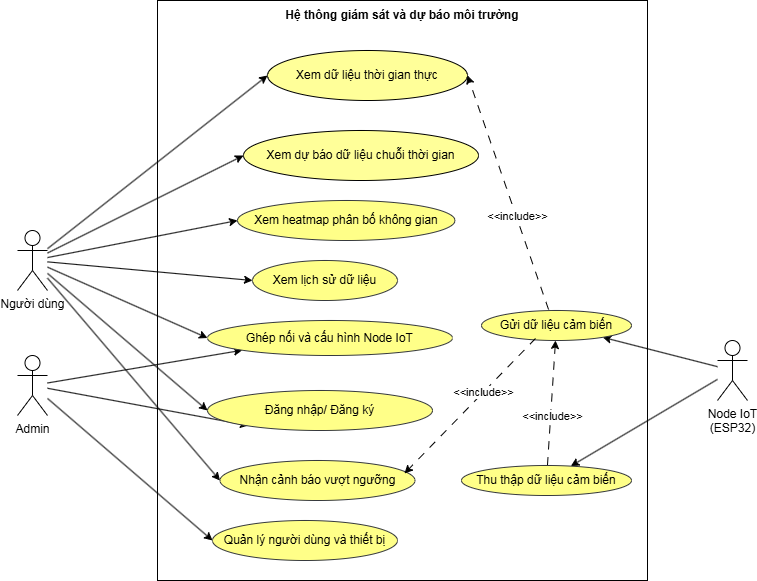
\includegraphics[width=0.9\textwidth]{uc_overall}
  \caption{Biểu đồ use case tổng quan của hệ thống}
  \label{fig:usecase_overall}
\end{figure}

Các chức năng chính của hệ thống bao gồm: đăng ký và cấu hình node IoT,
thu thập dữ liệu cảm biến theo thời gian thực, xem dữ liệu và biểu đồ
lịch sử, xem dự báo chuỗi thời gian, xem heatmap phân bố không gian,
và nhận cảnh báo khi vượt ngưỡng.

\subsection{Biểu đồ use case phân rã: Đăng ký và cấu hình node IoT}
\label{subsec:survey:uc:register}

Hình~\ref{fig:usecase_register} mô tả quy trình khởi tạo và quản lý
node IoT trong hệ thống. Chức năng trọng tâm là quá trình
\textit{provisioning} tự động: node ESP32 khi khởi động lần đầu sẽ
publish một thông điệp lên topic \texttt{devices/register} kèm địa chỉ
MAC. Backend Aedes broker lắng nghe topic này, kiểm tra xem thiết bị đã
tồn tại chưa, nếu chưa thì tạo bản ghi trong cơ sở dữ liệu, sinh
\texttt{api\_key} và gửi cấu hình (ngưỡng cảnh báo, phòng được gán) về
node qua topic \texttt{devices/\{mac\_address\}/config}.

\begin{figure}[H]
  \centering
  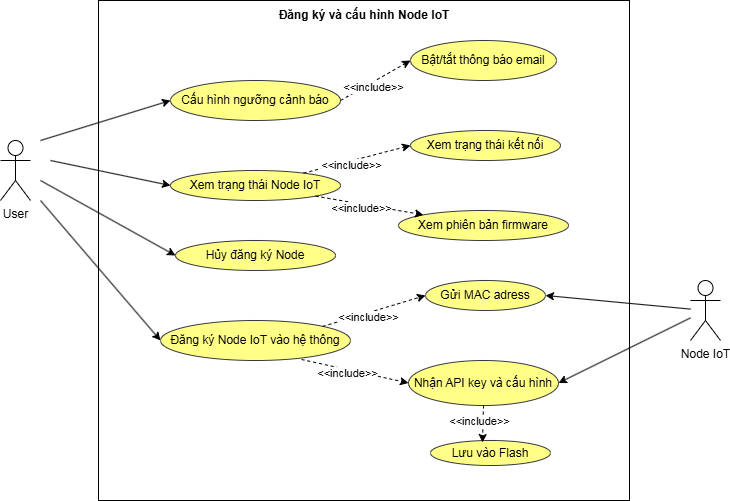
\includegraphics[width=0.9\textwidth]{uc_register}
  \caption{Biểu đồ use case phân rã: Đăng ký và cấu hình node IoT}
  \label{fig:usecase_register}
\end{figure}

Người dùng Admin có thể quản lý thiết bị qua dashboard: xem danh sách
node, chỉnh sửa ngưỡng cảnh báo nhiệt độ, độ ẩm (cao/thấp), gán node
vào phòng/khu vực, và vô hiệu hóa node khi cần.

\subsection{Biểu đồ use case phân rã: Thu thập dữ liệu và dự báo}
\label{subsec:survey:uc:collect}

Hình~\ref{fig:usecase_collect} minh họa quy trình thu thập dữ liệu tự
động từ node IoT và pipeline xử lý phía backend.

\begin{figure}[H]
  \centering
  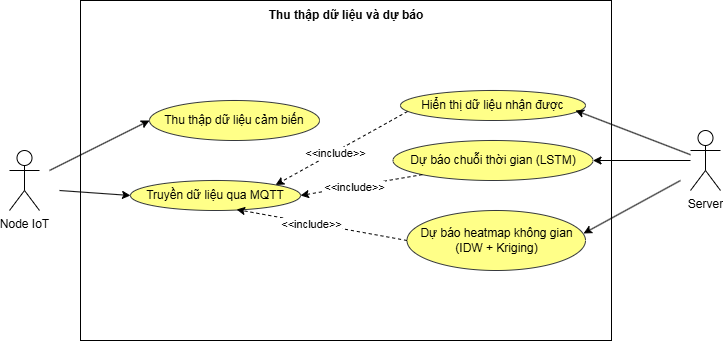
\includegraphics[width=0.9\textwidth]{uc_collect}
  \caption{Biểu đồ use case phân rã: Thu thập dữ liệu và dự báo}
  \label{fig:usecase_collect}
\end{figure}

Mỗi 5 giây, node ESP32 đọc dữ liệu từ cảm biến DHT11 và publish JSON
lên topic \texttt{device/\{api\_key\}/data}. Backend xác thực
\texttt{api\_key}, lưu vào bảng \texttt{readings} trong PostgreSQL,
đồng thời emit sự kiện \texttt{new\_reading} qua Socket.io đến các
client đang subscribe. Khi người dùng yêu cầu xem dự báo, backend gọi
FastAPI service, service này đọc 30 bản ghi gần nhất từ PostgreSQL,
đưa qua mô hình LSTM và trả về 15 giá trị dự báo tiếp theo.

\subsection{Biểu đồ use case phân rã: Xem dữ liệu và nhận cảnh báo}
\label{subsec:survey:uc:view}

Hình~\ref{fig:usecase_view} mô tả các chức năng tương tác chính của
người dùng với dashboard.

\begin{figure}[H]
  \centering
  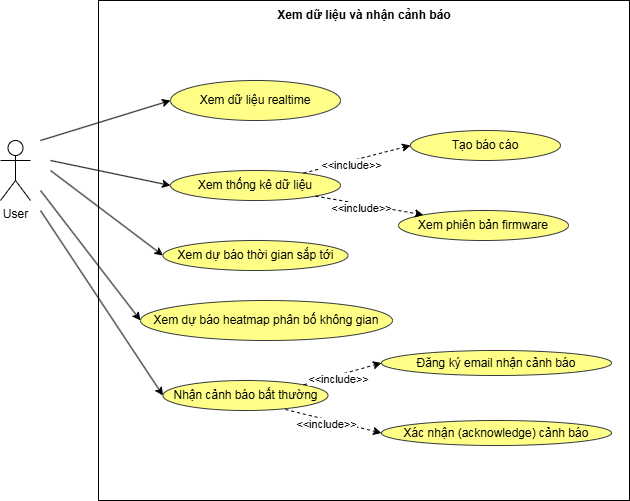
\includegraphics[width=0.9\textwidth]{uc_view}
  \caption{Biểu đồ use case phân rã: Xem dữ liệu và nhận cảnh báo}
  \label{fig:usecase_view}
\end{figure}

Người dùng có thể xem dữ liệu realtime qua biểu đồ Chart.js được cập
nhật tức thì thông qua Socket.io, xem lịch sử dữ liệu theo khoảng thời
gian tùy chọn, xem kết quả dự báo 15 phút tiếp theo, và xem heatmap
phân bố nhiệt độ, độ ẩm trong không gian phòng trên bản đồ Leaflet. Khi
các chỉ số vượt ngưỡng đã cài đặt, hệ thống tự động ghi alert vào cơ
sở dữ liệu, hiển thị thông báo trên dashboard và gửi email cảnh báo.

\subsection{Quy trình nghiệp vụ}
\label{subsec:survey:workflow}

\subsubsection*{a. Quy trình thu thập và xử lý dữ liệu}

Hình~\ref{fig:workflow_data} mô tả quy trình nghiệp vụ chính khi node
IoT gửi dữ liệu về hệ thống. Quy trình diễn ra hoàn toàn tự động và
liên tục theo chu kỳ 5 giây:

\begin{enumerate}[leftmargin=2cm]
  \item Node ESP32 đọc nhiệt độ, độ ẩm từ DHT11 và sinh giá trị AQI mô phỏng.
  \item ESP32 đóng gói JSON gồm nhiệt độ, độ ẩm, AQI và publish lên MQTT broker
    (Aedes) qua topic \texttt{device/\{api\_key\}/data}.
  \item Backend lắng nghe sự kiện \texttt{publish} của Aedes, xác thực
    \texttt{api\_key} với PostgreSQL.
  \item Nếu hợp lệ, bản ghi được lưu vào bảng \texttt{readings}.
  \item \texttt{alertService} kiểm tra giá trị vừa nhận với ngưỡng
    cài đặt của thiết bị. Nếu vượt ngưỡng, tạo bản ghi trong bảng
    \texttt{alerts} và gửi email thông báo.
  \item Socket.io emit sự kiện \texttt{new\_reading} đến tất cả client
    đang lắng nghe room \texttt{device\_\{id\}} và
    \texttt{user\_\{id\}}.
  \item Dashboard React nhận sự kiện, cập nhật biểu đồ Chart.js mà
    không cần tải lại trang.
\end{enumerate}

\begin{figure}[H]
  \centering
  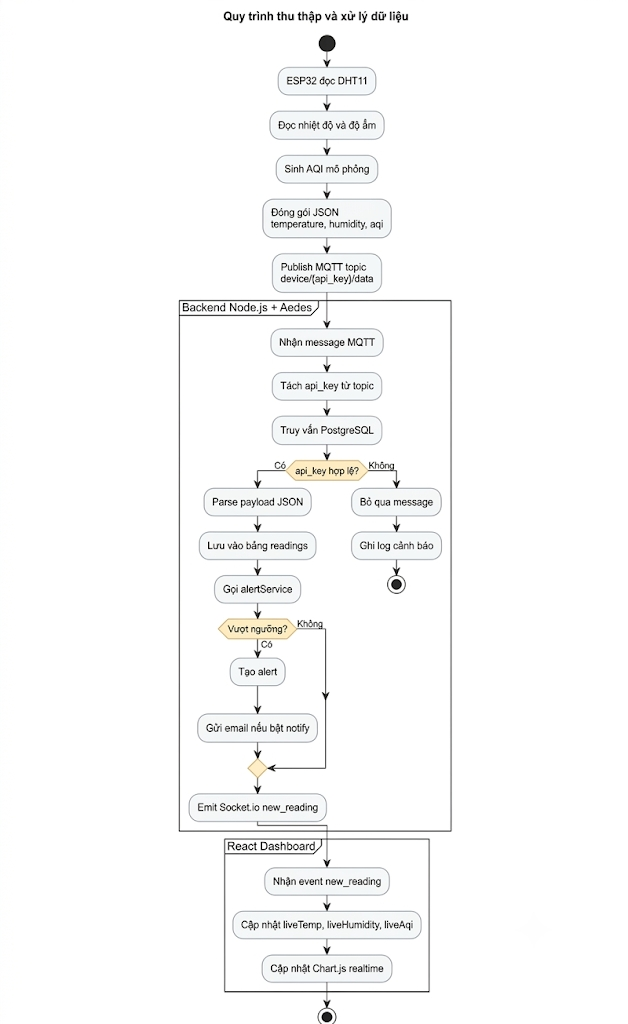
\includegraphics[width=\textwidth]{workflow_data}
  \caption{Quy trình nghiệp vụ thu thập và xử lý dữ liệu}
  \label{fig:workflow_data}
\end{figure}

\subsubsection*{b. Quy trình dự báo và nội suy không gian}

Hình~\ref{fig:workflow_forecast} mô tả quy trình khi người dùng yêu cầu
xem dự báo và heatmap phân bố không gian:

\begin{enumerate}[leftmargin=2cm]
  \item Người dùng mở trang dự báo hoặc trang heatmap trên dashboard.
  \item Frontend gọi REST API \texttt{GET /api/forecast} hoặc
    \texttt{GET /api/spatial-forecast} đến backend Node.js.
  \item Backend chuyển tiếp request tới FastAPI service: \texttt{forecast/main.py}
    cho dự báo trạm hoặc \texttt{forecast/spatial\_forecast.py} cho heatmap.
  \item FastAPI service truy vấn dữ liệu lịch sử 30 phút gần nhất từ PostgreSQL.
  \item Dữ liệu được chuẩn hóa qua \texttt{scaler.pkl}, đưa vào mô
    hình LSTM (PyTorch) để dự báo 15 phút tiếp theo.
  \item Với yêu cầu heatmap: kết hợp giá trị thực đo (hoặc dự báo) với
    tọa độ vị trí của từng node, áp dụng thuật toán IDW và Kriging để
    nội suy ra lưới dữ liệu 40$\times$50 điểm.
  \item Kết quả trả về dưới dạng JSON, frontend render lên bản đồ
    Leaflet dưới dạng heatmap màu sắc.
\end{enumerate}

\begin{figure}[H]
  \centering
  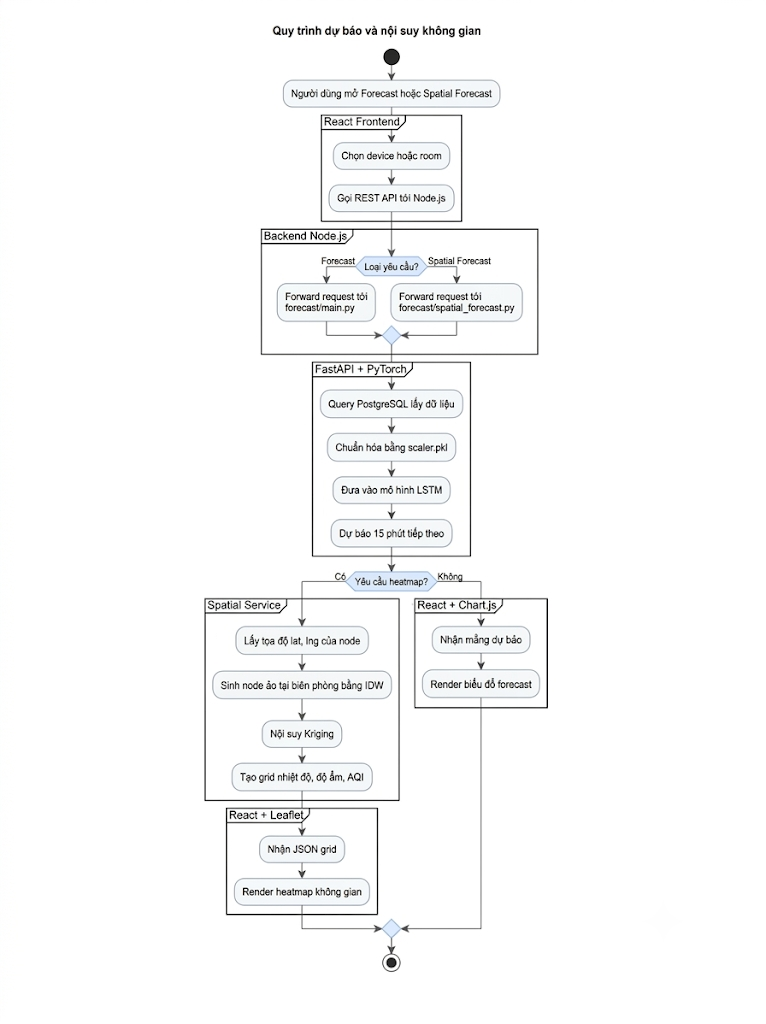
\includegraphics[width=\textwidth]{workflow_forecast}
  \caption{Quy trình nghiệp vụ dự báo và nội suy không gian}
  \label{fig:workflow_forecast}
\end{figure}

%------------------------------------------------------------
\section{Đặc tả chức năng}
\label{sec:survey:spec}
%------------------------------------------------------------

\subsection{Đặc tả use case UC01 - Đăng ký node IoT vào hệ thống}
\label{subsec:survey:uc01}

\begin{table}[H]
  \centering
  \caption{Đặc tả use case UC01: Đăng ký node IoT vào hệ thống}
  \label{tab:uc01}
  \begin{tabularx}{\textwidth}{p{4cm} X}
    \toprule
    \textbf{Mã use case}    & UC01 \\
    \midrule
    \textbf{Tên}            & Đăng ký node IoT vào hệ thống \\
    \textbf{Tác nhân}       & Node IoT (ESP32) \\
    \textbf{Mục đích}       & Cấp phát định danh và cấu hình ban đầu
                              cho node cảm biến mới \\
    \textbf{Tiền điều kiện} &
      \begin{minipage}[t]{\linewidth}
        \begin{enumerate}[leftmargin=*, topsep=0pt]
          \item ESP32 đã được cấp thông tin Wi-Fi qua AP cấu hình \texttt{Sensor-Setup-[MAC]}
          \item MQTT broker (Aedes) đang chạy và cho phép client provisioning kết nối
        \end{enumerate}
      \end{minipage} \\
    \textbf{Luồng chính}    &
      \begin{minipage}[t]{\linewidth}
        \begin{enumerate}[leftmargin=*, topsep=0pt]
          \item ESP32 khởi động, publish MAC address lên topic
            \texttt{devices/register}
          \item Aedes broker nhận message, kiểm tra MAC trong DB
          \item Nếu chưa tồn tại: tạo bản ghi device, sinh
            \texttt{api\_key} ngẫu nhiên, lưu vào bảng
            \texttt{devices}
          \item Backend publish cấu hình (ngưỡng, \texttt{api\_key})
            về topic \texttt{devices/\{mac\}/config}
          \item ESP32 nhận cấu hình, lưu vào Flash qua
            \texttt{Preferences.h}
        \end{enumerate}
      \end{minipage} \\
    \textbf{Luồng thay thế} &
      \begin{minipage}[t]{\linewidth}
        \begin{enumerate}[leftmargin=*, topsep=0pt]
          \item[3a.] MAC đã tồn tại: trả về cấu hình hiện có mà không
            tạo bản ghi mới
          \item[1a.] Wi-Fi không kết nối được: ESP32 retry sau 5 giây
        \end{enumerate}
      \end{minipage} \\
    \textbf{Hậu điều kiện} &
      \begin{minipage}[t]{\linewidth}
        \begin{enumerate}[leftmargin=*, topsep=0pt]
          \item Node được đăng ký trong hệ thống với \texttt{api\_key}
            duy nhất
          \item Node sẵn sàng gửi dữ liệu lên topic
            \texttt{device/\{api\_key\}/data}
        \end{enumerate}
      \end{minipage} \\
    \bottomrule
  \end{tabularx}
\end{table}

\subsection{Đặc tả use case UC02 - Thu thập và lưu trữ dữ liệu
cảm biến}
\label{subsec:survey:uc02}

\begin{table}[H]
  \centering
  \caption{Đặc tả use case UC02: Thu thập và lưu trữ dữ liệu cảm biến}
  \label{tab:uc02}
  \begin{tabularx}{\textwidth}{p{4cm} X}
    \toprule
    \textbf{Mã use case}    & UC02 \\
    \midrule
    \textbf{Tên}            & Thu thập và lưu trữ dữ liệu cảm biến \\
    \textbf{Tác nhân}       & Node IoT (ESP32), Hệ thống tự động \\
    \textbf{Mục đích}       & Đọc dữ liệu môi trường định kỳ và lưu
                              trữ vào cơ sở dữ liệu \\
    \textbf{Tiền điều kiện} &
      \begin{minipage}[t]{\linewidth}
        \begin{enumerate}[leftmargin=*, topsep=0pt]
          \item Node đã đăng ký thành công (UC01)
          \item Kết nối MQTT giữa node và broker ổn định
        \end{enumerate}
      \end{minipage} \\
    \textbf{Luồng chính}    &
      \begin{minipage}[t]{\linewidth}
        \begin{enumerate}[leftmargin=*, topsep=0pt]
          \item Mỗi 5 giây, ESP32 đọc nhiệt độ, độ ẩm từ DHT11 và sinh AQI mô phỏng
          \item Đóng gói thành JSON:
            \texttt{\{"temperature": x, "humidity": y, "aqi": z\}}
          \item Publish lên topic \texttt{device/\{api\_key\}/data}
          \item Aedes broker xác thực \texttt{api\_key}, lấy
            \texttt{device\_id} từ PostgreSQL
          \item Lưu bản ghi vào bảng \texttt{readings} với timestamp
          \item Gọi \texttt{alertService} kiểm tra ngưỡng
          \item Emit \texttt{new\_reading} qua Socket.io
        \end{enumerate}
      \end{minipage} \\
    \textbf{Luồng thay thế} &
      \begin{minipage}[t]{\linewidth}
        \begin{enumerate}[leftmargin=*, topsep=0pt]
          \item[4a.] \texttt{api\_key} không hợp lệ: bỏ qua message,
            ghi log cảnh báo
          \item[1a.] DHT11 lỗi đọc: bỏ qua chu kỳ này, thử lại sau
            5 giây
        \end{enumerate}
      \end{minipage} \\
    \textbf{Hậu điều kiện} &
      \begin{minipage}[t]{\linewidth}
        \begin{enumerate}[leftmargin=*, topsep=0pt]
          \item Dữ liệu được lưu bền vững trong PostgreSQL
          \item Các client kết nối nhận được dữ liệu realtime qua
            Socket.io
        \end{enumerate}
      \end{minipage} \\
    \bottomrule
  \end{tabularx}
\end{table}

\subsection{Đặc tả use case UC03 - Xem dự báo chuỗi thời gian và
heatmap không gian}
\label{subsec:survey:uc03}

\begin{table}[H]
  \centering
  \caption{Đặc tả use case UC03: Xem dự báo và heatmap không gian}
  \label{tab:uc03}
  \begin{tabularx}{\textwidth}{p{4cm} X}
    \toprule
    \textbf{Mã use case}    & UC03 \\
    \midrule
    \textbf{Tên}            & Xem dự báo chuỗi thời gian và heatmap
                              không gian \\
    \textbf{Tác nhân}       & Người dùng (User) \\
    \textbf{Mục đích}       & Cung cấp thông tin dự báo xu hướng môi
                              trường và phân bố không gian để hỗ trợ
                              quyết định \\
    \textbf{Tiền điều kiện} &
      \begin{minipage}[t]{\linewidth}
        \begin{enumerate}[leftmargin=*, topsep=0pt]
          \item Người dùng đã đăng nhập
          \item Có ít nhất 30 bản ghi trong PostgreSQL cho node
            cần dự báo
          \item FastAPI service đang chạy
        \end{enumerate}
      \end{minipage} \\
    \textbf{Luồng chính}    &
      \begin{minipage}[t]{\linewidth}
        \begin{enumerate}[leftmargin=*, topsep=0pt]
          \item Người dùng chọn node và nhấn ``Xem dự báo''
          \item Frontend gọi \texttt{GET /api/forecast?device\_id=\{id\}}
          \item Backend Node.js gọi FastAPI service (cổng 8000)
          \item FastAPI đọc 30 bản ghi gần nhất, chuẩn hóa qua
            \texttt{scaler.pkl}
          \item Mô hình LSTM suy luận, trả về mảng 15 giá trị dự báo
          \item Frontend hiển thị biểu đồ dự báo kết hợp với dữ liệu
            lịch sử
          \item Người dùng chọn tab ``Heatmap'': frontend gọi
            \texttt{GET /api/spatial-forecast}
          \item FastAPI tính Kriging/IDW, trả về lưới
            40$\times$50 điểm
          \item Leaflet render heatmap màu sắc trên bản đồ phòng
        \end{enumerate}
      \end{minipage} \\
    \textbf{Hậu điều kiện} &
      Người dùng xem được dự báo 15 phút tới và bản đồ nhiệt phân bố
      không gian \\
    \bottomrule
  \end{tabularx}
\end{table}

%------------------------------------------------------------
\section{Yêu cầu phi chức năng}
\label{sec:survey:nonfunc}
%------------------------------------------------------------

Hệ thống được xây dựng cần đảm bảo các yêu cầu phi chức năng sau:

\textbf{Hiệu năng:} Độ trễ từ khi node gửi dữ liệu đến khi dashboard
cập nhật không vượt quá 2 giây trong điều kiện mạng bình thường. Thời
gian phản hồi của các API thông thường dưới 500ms. Thời gian suy luận
LSTM (15 phút dự báo) dưới 1 giây. Hệ thống hỗ trợ tối thiểu 10 node
IoT hoạt động đồng thời.

\textbf{Độ tin cậy:} Dữ liệu cảm biến phải được lưu trữ đầy đủ, không
mất mát trong điều kiện mạng ổn định. Khi node IoT mất kết nối MQTT,
thiết bị tự động thử kết nối lại (reconnect) theo cơ chế backoff. Hệ
thống cảnh báo phải gửi email trong vòng 30 giây kể từ khi phát hiện
vượt ngưỡng.

\textbf{Bảo mật:} Tất cả API endpoint yêu cầu xác thực JWT. Mật khẩu
người dùng được mã hóa bằng bcrypt trước khi lưu vào cơ sở dữ liệu.
Mỗi node IoT được định danh bằng \texttt{api\_key} duy nhất, được xác
thực tại backend trước khi chấp nhận dữ liệu.

\textbf{Khả năng sử dụng:} Giao diện dashboard phải trực quan, hiển thị
dữ liệu realtime mà không cần tải lại trang. Biểu đồ và heatmap phải
phản hồi ngay lập tức khi có dữ liệu mới. Hệ thống cảnh báo hiển thị
rõ ràng thông tin node, loại cảnh báo và thời điểm xảy ra.

\textbf{Khả năng mở rộng:} Kiến trúc phải cho phép bổ sung node cảm
biến mới mà không cần thay đổi code backend. Cơ sở dữ liệu PostgreSQL
được thiết kế để hỗ trợ truy vấn dữ liệu lịch sử hiệu quả với chỉ mục
phù hợp trên cột \texttt{timestamp} và \texttt{device\_id}.

\textbf{Chi phí:} Tổng chi phí phần cứng cho một node cảm biến (ESP32 +
DHT11 + nguồn) không vượt quá 150.000 VND, đảm bảo khả năng triển khai
mật độ cao với ngân sách hạn chế.

%============================================================
% CHƯƠNG 3: THIẾT KẾ VÀ TRIỂN KHAI HỆ THỐNG
%============================================================
\chapter{THIẾT KẾ VÀ TRIỂN KHAI HỆ THỐNG}
\label{chap:design}

Chương này trình bày toàn bộ quá trình thiết kế và xây dựng hệ thống
AIoT giám sát và dự báo chất lượng không khí. Nội dung bao gồm thiết
kế kiến trúc tổng thể theo mô hình bốn tầng, thiết kế chi tiết từng
thành phần tích hợp chặt chẽ với các phân tích lựa chọn công nghệ tương ứng (vi
điều khiển, cảm biến, giao thức truyền thông, cơ sở dữ liệu, backend, mô hình dự
báo học sâu và giao diện trực quan), kết quả xây dựng hệ thống và quy
trình triển khai chi tiết.

%------------------------------------------------------------
\section{Thiết kế kiến trúc}
\label{sec:design:arch}
%------------------------------------------------------------

\subsection{Lựa chọn kiến trúc phần mềm}
\label{subsec:design:arch:choice}

Hệ thống được thiết kế theo \textbf{kiến trúc bốn tầng} kết hợp mô
hình IoT Gateway, thể hiện trong Hình~\ref{fig:arch_overview}. Kiến
trúc này phân tách rõ ràng trách nhiệm của từng tầng, đảm bảo khả năng
mở rộng độc lập và dễ bảo trì:

\begin{enumerate}[leftmargin=2cm]
  \item \textbf{Tầng thu thập (Edge Layer):} Node cảm biến đọc dữ liệu và gửi lên qua kết nối mạng không dây. Tầng này hoạt động hoàn toàn tự động, không cần can thiệp người dùng sau khi cấu hình ban đầu.
  \item \textbf{Tầng truyền dẫn (Transport Layer):} Giao thức truyền thông nhẹ đảm bảo truyền dữ liệu nhanh, độ trễ thấp và hỗ trợ nhiều node đồng thời.
  \item \textbf{Tầng xử lý và lưu trữ (Backend Layer):} Hệ thống máy chủ trung tâm xử lý nghiệp vụ, cơ sở dữ liệu lưu trữ dữ liệu chuỗi thời gian, và các API microservice chạy mô hình học sâu suy luận và thuật toán nội suy không gian.
  \item \textbf{Tầng hiển thị (Presentation Layer):} Giao diện Web Dashboard nhận dữ liệu và cập nhật trực quan realtime dưới dạng biểu đồ và bản đồ nhiệt.
\end{enumerate}

\begin{figure}[H]
  \centering
  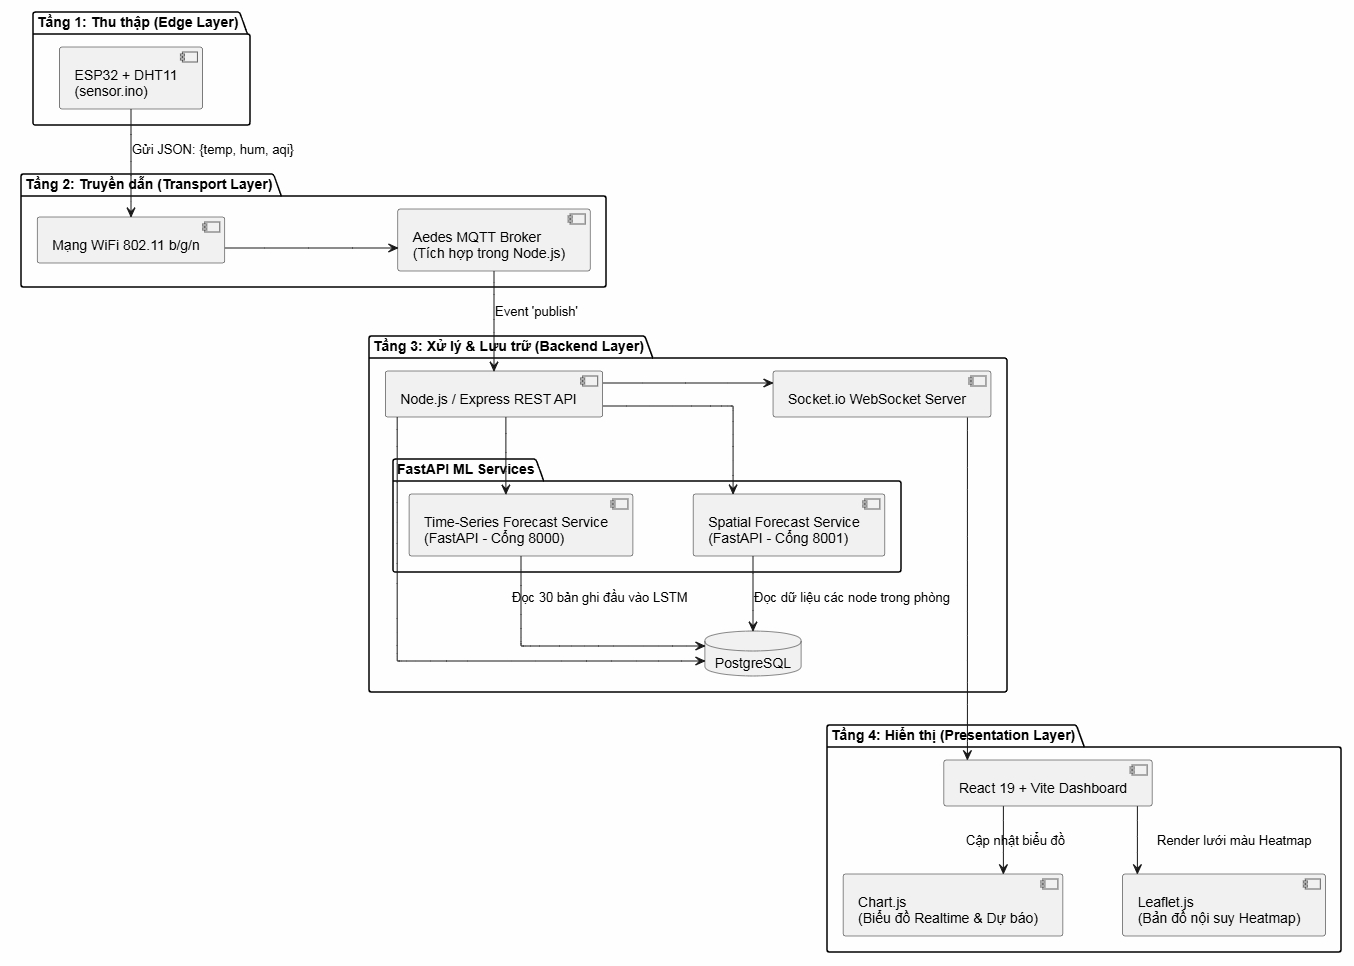
\includegraphics[width=0.95\textwidth]{arch_overview}
  \caption{Kiến trúc tổng quan của hệ thống AIoT giám sát và dự báo chất lượng không khí}
  \label{fig:arch_overview}
\end{figure}

Lý do lựa chọn kiến trúc này so với các phương án khác:

\begin{itemize}[leftmargin=2cm]
  \item \textbf{So với kiến trúc monolithic:} Việc tách riêng dịch vụ Machine Learning độc lập khỏi máy chủ backend chính giúp đảm bảo hiệu năng xử lý, tránh block luồng chạy chính khi chạy suy luận nặng.
  \item \textbf{So với kiến trúc serverless:} Hệ thống cần duy trì kết nối truyền thông liên tục và tức thời (realtime), không phù hợp với mô hình stateless của serverless.
  \item \textbf{So với Cloud-only:} Broker tích hợp trực tiếp trong backend giúp giảm bớt một hop mạng trung gian, từ đó giảm thiểu độ trễ truyền dữ liệu đầu cuối.
\end{itemize}

\subsection{Thiết kế tổng quan các gói}
\label{subsec:design:arch:packages}

Hình~\ref{fig:package_diagram} mô tả biểu đồ phụ thuộc gói tổng quan
của hệ thống, phân chia thành bốn nhóm chính tương ứng với bốn tầng
kiến trúc.

\begin{figure}[H]
  \centering
  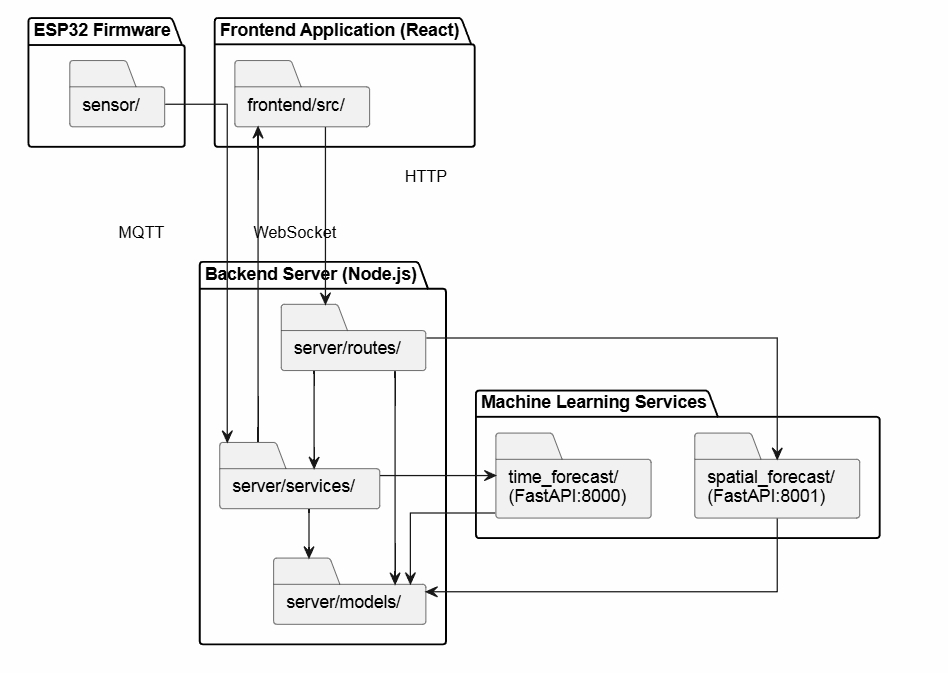
\includegraphics[width=0.95\textwidth]{package_diagram}
  \caption{Biểu đồ phụ thuộc gói tổng quan của hệ thống}
  \label{fig:package_diagram}
\end{figure}

Cấu trúc thư mục dự án phản ánh trực tiếp kiến trúc này:

\begin{itemize}[leftmargin=2cm]
  \item \texttt{sensor/} --- Firmware thiết bị vi điều khiển (C/C++)
  \item \texttt{server/} --- Backend chính điều phối nghiệp vụ (JavaScript)
    \begin{itemize}
      \item \texttt{controllers/} --- Xử lý HTTP request
      \item \texttt{routes/} --- Định nghĩa API endpoint
      \item \texttt{services/} --- Logic nghiệp vụ (cảnh báo, kết nối truyền thông, dự báo)
      \item \texttt{middleware/} --- Xác thực, phân quyền bảo mật
      \item \texttt{models/} --- Giao tiếp cơ sở dữ liệu
    \end{itemize}
  \item \texttt{lstm\_train/} --- Pipeline Machine Learning (huấn luyện, suy luận và nội suy)
  \item \texttt{frontend/src/} --- Mã nguồn giao diện Web Dashboard (React)
    \begin{itemize}
      \item \texttt{pages/} --- Các màn hình chức năng chính
      \item \texttt{components/} --- Các thành phần UI dùng lại
      \item \texttt{context/} --- Quản lý trạng thái toàn cục
    \end{itemize}
\end{itemize}

%------------------------------------------------------------
\section{Thiết kế chi tiết}
\label{sec:design:detail}
%------------------------------------------------------------

\subsection{Thiết kế phần cứng node cảm biến}
\label{subsec:design:hardware}

\subsubsection*{a. Lựa chọn và đặc tả chi tiết linh kiện phần cứng}

Node cảm biến được thiết kế dựa trên sự kết hợp giữa hiệu năng xử lý, khả năng kết nối mạng không dây và tối ưu hóa chi phí triển khai thực tế.
\begin{itemize}[leftmargin=2cm]
  \item \textbf{Vi điều khiển ESP32:} ESP32 là dòng vi điều khiển (SoC) do Espressif Systems phát triển, tích hợp bộ xử lý lõi kép Xtensa LX6 32-bit hoạt động ở tần số lên đến 240~MHz, cùng với Wi-Fi 802.11 b/g/n và Bluetooth 4.2/BLE trên cùng một chip~\cite{espressif2024esp32}. Các thông số kỹ thuật quan trọng bao gồm 520~KB SRAM, hỗ trợ Flash ngoài thông thường 4--16~MB, và đầy đủ các giao tiếp ngoại vi như I2C, SPI, UART, ADC, DAC.
  
  \textit{Lý do lựa chọn cho đồ án:}
  \begin{itemize}
    \item \textbf{Tích hợp Wi-Fi sẵn:} Cho phép kết nối MQTT trực tiếp đến broker mà không cần module truyền thông bổ sung, giảm chi phí và độ phức tạp phần cứng.
    \item \textbf{Chi phí thấp:} Giá thành module ESP32 trên thị trường Việt Nam khoảng 50.000--80.000 VND, phù hợp triển khai nhiều node.
    \item \textbf{Hệ sinh thái phong phú:} Được hỗ trợ đầy đủ bởi Arduino IDE với thư viện MQTT (\texttt{PubSubClient}), JSON (\texttt{ArduinoJson}) và cảm biến DHT đã trưởng thành.
    \item \textbf{Bộ nhớ Flash đủ dùng:} Thư viện \texttt{Preferences.h} cho phép lưu cấu hình định danh (\texttt{device\_id}, \texttt{api\_key} và địa chỉ \texttt{mqtt\_server}) vào Flash bền vững qua các lần reset.
  \end{itemize}

  \item \textbf{Cảm biến DHT11:} DHT11 là cảm biến kỹ thuật số đo nhiệt độ và độ ẩm tương đối sử dụng giao tiếp 1-Wire~\cite{dht11datasheet}. Thông số kỹ thuật chính được thể hiện ở Bảng~\ref{tab:dht11_spec}.
  
  \begin{table}[H]
    \centering
    \caption{Thông số kỹ thuật cảm biến DHT11}
    \label{tab:dht11_spec}
    \begin{tabular}{lll}
      \toprule
      \textbf{Thông số} & \textbf{Giá trị} & \textbf{Đơn vị} \\
      \midrule
      Dải đo nhiệt độ   & 0 - 50          & $^\circ$C       \\
      Độ chính xác nhiệt độ & $\pm$2       & $^\circ$C       \\
      Dải đo độ ẩm      & 20 - 80         & \%RH            \\
      Độ chính xác độ ẩm & $\pm$5          & \%RH            \\
      Điện áp hoạt động & 3.3 - 5         & V               \\
      Giao tiếp         & 1-Wire (Digital) & -             \\
      Tần suất lấy mẫu  & 1                & lần/giây tối đa \\
      \bottomrule
    \end{tabular}
  \end{table}

  DHT11 được lựa chọn vì giá thành rất thấp (khoảng 15.000--25.000 VND), dễ kết nối với ESP32 qua một chân digital duy nhất (GPIO4 trong đồ án), và thư viện \texttt{DHT.h} đã ổn định, dễ tích hợp. Mặc dù độ chính xác không bằng DHT22, DHT11 đủ đáp ứng yêu cầu của hệ thống quan trắc môi trường prototype trong phạm vi đồ án.
\end{itemize}

\subsubsection*{b. Sơ đồ kết nối phần cứng}

Node cảm biến kết nối cảm biến DHT11 trực tiếp tới một chân đầu vào kỹ thuật số (GPIO4) của ESP32 qua điện trở kéo lên (pull-up) $10\text{k}\Omega$ để đảm bảo tính ổn định của đường truyền 1-Wire. Sơ đồ kết nối chi tiết được minh họa trong Hình~\ref{fig:hardware_schematic}.

\begin{figure}[H]
  \centering
  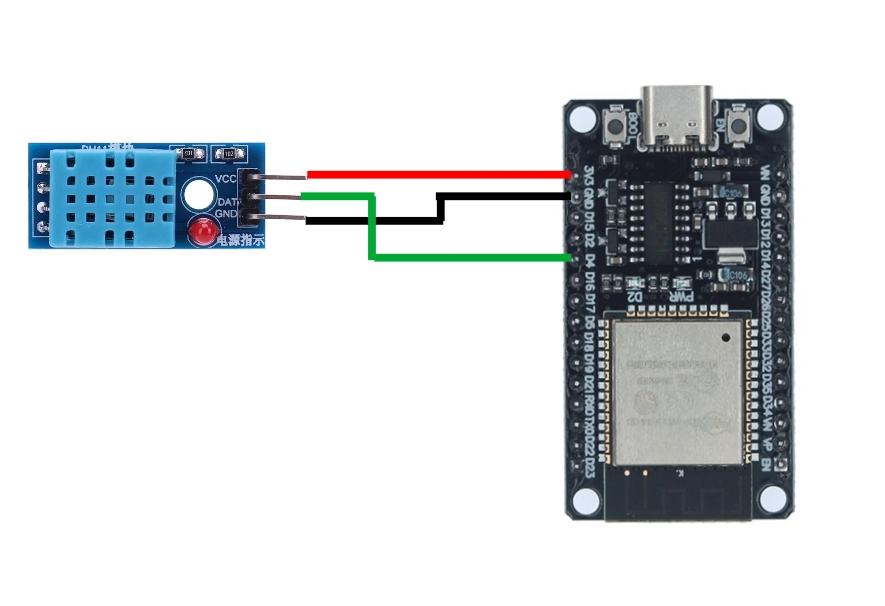
\includegraphics[width=0.7\textwidth]{hardware_schematic}
  \caption{Sơ đồ kết nối phần cứng node cảm biến}
  \label{fig:hardware_schematic}
\end{figure}

Bảng~\ref{tab:gpio_config} liệt kê cấu hình chân kết nối:

\begin{table}[H]
  \centering
  \caption{Cấu hình chân kết nối ESP32 --- DHT11}
  \label{tab:gpio_config}
  \begin{tabular}{llll}
    \toprule
    \textbf{Chân DHT11} & \textbf{Chân ESP32} & \textbf{Chức năng}
      & \textbf{Ghi chú} \\
    \midrule
    VCC  & 3.3V   & Nguồn cấp      & --- \\
    DATA & GPIO4  & Dữ liệu 1-Wire & Qua điện trở 10k$\Omega$ pull-up \\
    GND  & GND    & Nối đất        & --- \\
    \bottomrule
  \end{tabular}
\end{table}

\subsubsection*{c. Cơ chế lưu cấu hình định danh trên Flash}

Để node cảm biến hoạt động tự động sau khi khởi động lại hoặc mất nguồn điện, thiết bị cần lưu trữ mã khóa xác thực định danh (\texttt{api\_key}) và cấu hình nhận từ máy chủ. Chúng tôi sử dụng thư viện \texttt{Preferences.h} của ESP32 để ghi dữ liệu trực tiếp vào phân vùng NVS (Non-Volatile Storage) trên bộ nhớ Flash. Thuật toán đọc và ghi cấu hình được mô tả dưới dạng mã giả ở mã nguồn giải thuật bên dưới:

\begin{lstlisting}[language=C, caption={Giai thuat luu va doc cau hinh dinh danh tren Flash}, label={lst:preferences_pseudo}]
Ham docCauHinhTuFlash()
    Mo vung luu tru "device" o che do chi doc (read-only)
    deviceId = Doc gia tri so nguyen voi khoa "device_id" (mac dinh = -1)
    deviceApiKey = Doc chuoi ky tu voi khoa "api_key" (mac dinh = "")
    Dong vung luu tru
Ket thuc Ham

Ham ghiCauHinhVaoFlash(idMoi, keyMoi)
    Mo vung luu tru "device" o che do ghi-doc (read-write)
    Ghi idMoi vao khoa "device_id"
    Ghi keyMoi vao khoa "api_key"
    Dong vung luu tru
Ket thuc Ham
\end{lstlisting}

\subsection{Thiết kế Firmware}
\label{subsec:design:firmware}

\subsubsection*{a. Giao thức truyền thông MQTT và cấu trúc Topics}

Hệ thống sử dụng giao thức truyền thông \textbf{MQTT} (Message Queuing Telemetry Transport) cho việc truyền dẫn dữ liệu từ các node cảm biến lên máy chủ~\cite{banks2014mqtt}. MQTT hoạt động trên mô hình Publish/Subscribe qua nền tảng TCP/IP, có kích thước tiêu đề gói tin (overhead) cực nhẹ (chỉ tối thiểu 2 byte), giúp tối ưu hóa băng thông truyền tải và giảm điện năng tiêu thụ cho thiết bị. Hệ thống sử dụng thư viện \texttt{PubSubClient} tích hợp trên ESP32 để kết nối đến máy chủ trung tâm. Cấu trúc các topic truyền tin được định nghĩa trong Bảng~\ref{tab:mqtt_topics}.

\begin{table}[H]
  \centering
  \caption{Cấu trúc MQTT topic trong hệ thống}
  \label{tab:mqtt_topics}
  \begin{tabularx}{\textwidth}{p{6cm} p{2cm} X}
    \toprule
    \textbf{Topic} & \textbf{Chiều} & \textbf{Mô tả} \\
    \midrule
    \texttt{devices/register}
      & Node $\to$ Máy chủ
      & Node mới gửi MAC address để đăng ký tự động \\
    \texttt{devices/\{mac\}/config}
      & Máy chủ $\to$ Node
      & Máy chủ trả lời \texttt{api\_key} và thông số cấu hình \\
    \texttt{device/\{api\_key\}/data}
      & Node $\to$ Máy chủ
      & Gửi dữ liệu nhiệt độ, độ ẩm và AQI định kỳ \\
    \bottomrule
  \end{tabularx}
\end{table}

MQTT broker được tích hợp trực tiếp vào backend Node.js thông qua thư viện \textbf{Aedes} - một broker MQTT thuần Node.js hiệu năng cao, không yêu cầu cài đặt broker riêng biệt (như Mosquitto), giúp đơn giản hóa việc triển khai và tích hợp chặt chẽ với logic nghiệp vụ.

\subsubsection*{b. Luồng xử lý chính của firmware}

Firmware được tổ chức theo kiến trúc phân tầng như minh họa trong
Hình~\ref{fig:firmware_arch}. Vòng lặp chính (\texttt{loop()}) điều
phối ba tác vụ theo chu kỳ: đọc cảm biến, duy trì kết nối MQTT và
gửi dữ liệu.

\begin{figure}[H]
  \centering
  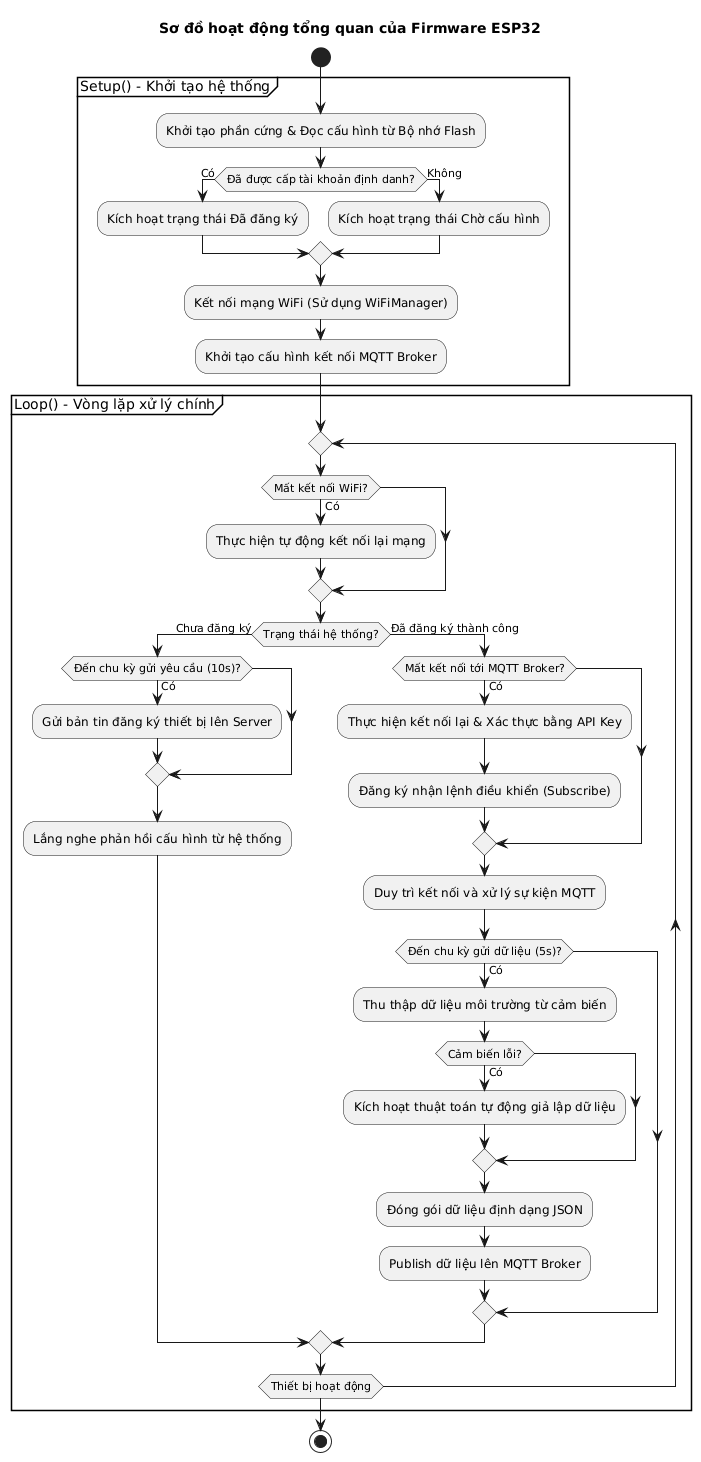
\includegraphics[width=0.75\textwidth]{firmware_arch}
  \caption{Kiến trúc firmware phân tầng của node ESP32}
  \label{fig:firmware_arch}
\end{figure}

Giải thuật vận hành chính của firmware được mô tả qua mã giả dưới đây:

\begin{lstlisting}[language=C, caption={Giai thuat vong lap chinh dieu phoi firmware ESP32}, label={lst:firmware_main_pseudo}]
Ham setup()
    Khoi tao giao tiep cam bien DHT
    docCauHinhTuFlash()
    Neu chua co thong tin Wi-Fi:
        Khoi chay AP "Sensor-Setup-[MAC]" de nguoi dung cau hinh mang
    Cau hinh ket noi toi may chu MQTT Broker va dang ky ham callback nhan tin
Ket thuc Ham

Ham loop()
    Neu chua co thong tin dang ky (api_key trong):
        guiYeuCauDangKyToiTopic("devices/register") kem dia chi MAC
        Cho 5 giay roi thu lai
        Tra ve
    Neu ket noi MQTT bi ngat:
        Thuc hien ket noi lai bang tai khoan xac thuc api_key
    Duy tri trang thai ket noi MQTT (mqttClient.loop())

    Neu thoi gian hien tai - thoi diem gui cuoi cung >= 5 giay:
        nhietDo = docNhietDoTuCamBien()
        doAm = docDoAmTuCamBien()
        aqi = sinhDuLieuAQIMoPhong()  // Danh cho pipeline ML
        
        Neu nhietDo va doAm hop le (khong phai NaN):
            goiTin = Dong goi JSON { "temperature": nhietDo, "humidity": doAm, "aqi": aqi }
            guiGoiTinToiTopic("device/" + api_key + "/data", goiTin)
        Cap nhat thoi diem gui cuoi cung
Ket thuc Ham
\end{lstlisting}
*Mã nguồn C++ chi tiết điều phối vòng lặp và logic gửi tin được đính kèm tại Phụ lục~\ref{lst:firmware_main}.*

\subsubsection*{c. Xử lý tin nhắn cấu hình nhận được}

Khi nhận cấu hình từ topic \texttt{devices/\{mac\}/config}, callback
MQTT giải mã thông điệp JSON để lưu thông tin định danh thiết bị vào Flash, đặt cờ đăng ký thành công (\texttt{provisioned}) để chuyển sang chế độ gửi dữ liệu, hoặc thực hiện đặt lại thiết bị (reset) khi có yêu cầu:

\begin{lstlisting}[language=C, caption={Giai thuat callback xu ly thong diep cau hinh tu MQTT Broker}, label={lst:mqtt_callback_pseudo}]
Ham callbackNhanTin(topic, goiTin)
    Giai ma goi tin JSON nhan duoc
    Neu goi tin co lenh reset ("action" == "reset"):
        Mo vung luu tru "device" o che do ghi-doc
        Xoa toan bo cau hinh luu tru
        Dong vung luu tru
        Khoi dong lai thiet bi (ESP.restart())
        Tra ve
        
    Neu goi tin chua "device_id" va "api_key":
        ghiCauHinhVaoFlash(device_id, api_key)
        Cap nhat bien trang thai: deviceId = device_id, deviceApiKey = api_key
        Dat trang thai dang ky thanh cong (provisioned = True)
Ket thuc Ham
\end{lstlisting}

\subsection{Thiết kế cơ sở dữ liệu}
\label{subsec:design:database}

\subsubsection*{a. Lựa chọn PostgreSQL lưu trữ dữ liệu}

Hệ thống lựa chọn hệ quản trị cơ sở dữ liệu quan hệ \textbf{PostgreSQL} để lưu trữ toàn bộ dữ liệu người dùng, cấu hình thiết bị và dữ liệu chuỗi thời gian đo đạc được~\cite{postgresql}. PostgreSQL được lựa chọn cho đồ án vì:
\begin{itemize}[leftmargin=2cm]
  \item Hỗ trợ đầy đủ SQL chuẩn, dễ truy vấn dữ liệu lịch sử theo khoảng thời gian với câu lệnh \texttt{WHERE timestamp BETWEEN ... AND ...}.
  \item Tích hợp tốt với Node.js qua thư viện \texttt{pg} (PostgreSQL client).
  \item Hỗ trợ tạo chỉ mục (index) trên cột \texttt{timestamp} và \texttt{device\_id} giúp tăng tốc truy vấn dữ liệu chuỗi thời gian cho các phép toán học sâu và nội suy.
  \item Miễn phí, phổ biến, có độ ổn định cực cao và dễ triển khai trên môi trường local cũng như VPS.
\end{itemize}

\subsubsection*{b. Sơ đồ ERD}

Cơ sở dữ liệu PostgreSQL gồm 5 bảng chính, quan hệ được thể hiện trong Hình~\ref{fig:erd}.

\begin{figure}[H]
  \centering
  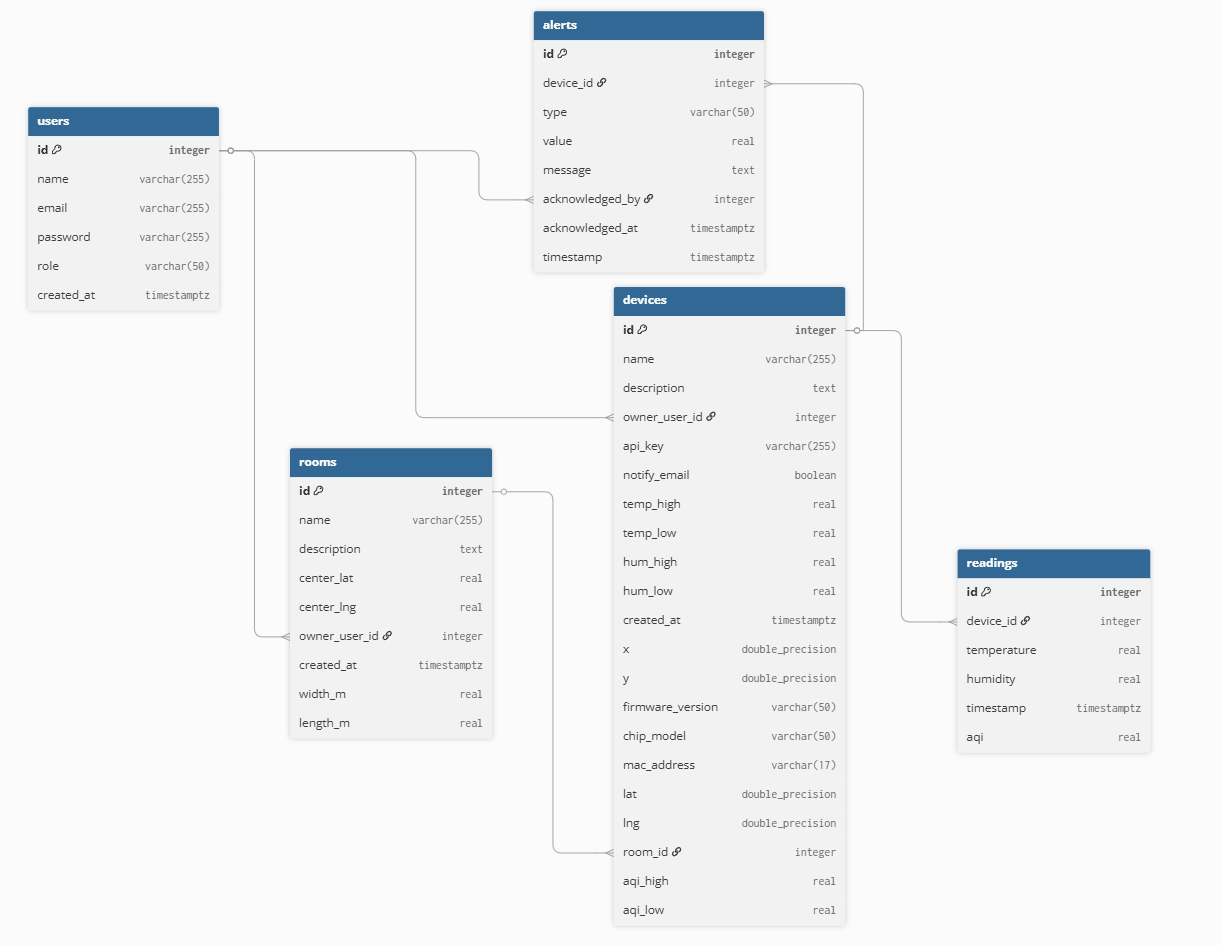
\includegraphics[width=\textwidth]{erd}
  \caption{Sơ đồ ERD cơ sở dữ liệu PostgreSQL}
  \label{fig:erd}
\end{figure}

\subsubsection*{c. Định nghĩa schema cơ sở dữ liệu}

Cấu trúc các bảng trong cơ sở dữ liệu được định nghĩa chi tiết tại Phụ lục~\ref{lst:schema}. Mối quan hệ giữa các bảng được thiết lập như sau:
\begin{itemize}[leftmargin=2cm]
  \item \texttt{users} $\to$ \texttt{devices}: Một người dùng (tài khoản) có thể sở hữu và quản lý nhiều node thiết bị cảm biến khác nhau. Ràng buộc khóa ngoại \texttt{owner\_user\_id} tham chiếu đến bảng \texttt{users}.
  \item \texttt{rooms} $\to$ \texttt{devices}: Một phòng có thể đặt nhiều node cảm biến để tăng mật độ và độ bao phủ không gian phục vụ bài toán nội suy. Mỗi thiết bị được định vị bằng toạ độ tương đối $(x, y)$ trong phòng thông qua khóa ngoại \texttt{room\_id}.
  \item \texttt{devices} $\to$ \texttt{readings}: Ràng buộc một-nhiều, lưu trữ lịch sử chuỗi thời gian các chỉ số đo đạc theo từng mã thiết bị. Chỉ mục \texttt{idx\_readings\_device\_time} được tạo trên cặp cột \texttt{(device\_id, timestamp DESC)} giúp tăng tốc độ truy vấn 30 mẫu gần nhất phục vụ mô hình dự báo.
  \item \texttt{devices} $\to$ \texttt{alerts}: Lưu lại lịch sử các sự kiện cảnh báo bất thường khi chỉ số môi trường vượt ngưỡng.
\end{itemize}

\subsection{Thiết kế Backend API}
\label{subsec:design:backend}

\subsubsection*{a. Cấu trúc và công nghệ của Backend chính}

Máy chủ backend chính được xây dựng trên môi trường \textbf{Node.js} sử dụng framework \textbf{Express} để xây dựng kiến trúc RESTful API phục vụ các tác vụ xác thực, quản lý người dùng, cấu hình thiết bị và trung chuyển dữ liệu~\cite{nodejs}. Node.js sử dụng kiến trúc bất đồng bộ hướng sự kiện (event-driven, non-blocking I/O) giúp xử lý hàng ngàn kết nối đồng thời từ client và thiết bị với mức tiêu tốn tài nguyên tối thiểu.

Các thư viện npm chính được sử dụng để phát triển backend bao gồm:
\begin{itemize}[leftmargin=2cm]
  \item \textbf{aedes + mqtt:} MQTT broker và client tích hợp trực tiếp trong cùng tiến trình Node.js giúp xử lý sự kiện trong cùng vòng lặp sự kiện, tối thiểu hóa độ trễ trung gian.
  \item \textbf{socket.io:} Thư viện WebSocket hỗ trợ giao tiếp hai chiều, realtime để phân phối dữ liệu ngay lập tức tới dashboard của client mà không cần cơ chế polling~\cite{socketio}.
  \item \textbf{pg:} PostgreSQL client cho Node.js phục vụ giao tiếp DB.
  \item \textbf{jsonwebtoken + bcrypt:} Xác thực an toàn bằng mã khóa JWT và băm mật khẩu bảo vệ tài khoản.
  \item \textbf{nodemailer:} Dịch vụ gửi email cảnh báo tự động khi các chỉ số đo đạc vượt quá ngưỡng an toàn được cài đặt.
\end{itemize}

Các API endpoint được phân chia thành ba nhóm chính, phân quyền truy cập thông qua mã xác thực JWT:
\begin{itemize}[leftmargin=2cm]
  \item \textbf{Quản lý người dùng và xác thực:} Các API \texttt{/api/auth/register}, \texttt{/api/auth/login} để đăng ký và đăng nhập nhận mã token bảo mật.
  \item \textbf{Quản lý thiết bị và phòng học:} Các API \texttt{GET, POST, PUT, DELETE /api/devices} và \texttt{/api/rooms} để xem danh sách, đăng ký và cấu hình toạ độ/ngưỡng cảnh báo cho từng node cảm biến.
  \item \textbf{Dữ liệu môi trường, dự báo và cảnh báo:} API \texttt{GET /api/data} truy vấn lịch sử đo, API \texttt{GET /api/forecast} gọi FastAPI LSTM service để lấy kết quả dự báo thời gian, và API \texttt{GET /api/spatial-forecast} gọi FastAPI spatial service lấy dữ liệu lưới nhiệt độ/độ ẩm không gian.
\end{itemize}

\subsubsection*{b. Xác thực người dùng bằng JWT}

Xác thực phía API sử dụng cơ chế token JWT (JSON Web Token) để đảm bảo tính an toàn cho tài nguyên. Giải thuật trung gian xác thực (middleware) được mô tả qua mã giả dưới đây:

\begin{lstlisting}[language=JavaScript, caption={Giai thuat middleware xac thuc nguoi dung bang token JWT}, label={lst:jwt_middleware_pseudo}]
Ham xacThucTokenJWT(yeuCau, phanHoi, hamTiepTheo)
    chuoiXacThuc = Lay Authorization tu yeuCau.headers
    Neu chuoiXacThuc khong ton tai:
        Tra ve phanHoi voi ma loi 401 ("Missing token")
        
    token = Trich xuat phan chuoi sau tu "Bearer <token>"
    Thu:
        thongTinGiaiMa = Giai ma token bang khoa bi mat JWT_SECRET
        Gan yeuCau.user = thongTinGiaiMa
        Chuyen tiep den hamTiepTheo()
    Neu xay ra loi giai ma:
        Tra ve phanHoi voi ma loi 403 ("Invalid token")
Ket thuc Ham
\end{lstlisting}

\subsubsection*{c. Logic tự động phát hiện vượt ngưỡng cảnh báo}

Dịch vụ cảnh báo (\texttt{alertService.js}) được khởi chạy bất đồng bộ mỗi khi backend nhận được bản ghi dữ liệu đo đạc mới từ node cảm biến thông qua MQTT. Dịch vụ đối chiếu giá trị đo với các ngưỡng cấu hình lưu trong cơ sở dữ liệu để đưa ra quyết định gửi thông báo qua giao diện và gửi email cảnh báo tự động:

\begin{lstlisting}[language=JavaScript, caption={Giai thuat kiem tra va kich hoat canh bao tu dong}, label={lst:alert_service_pseudo}]
Ham kiemTraNguongCanhBao(thietBi, duLieuDo)
    nhietDo = duLieuDo.temperature
    doAm = duLieuDo.humidity
    danhSachCanhBao = []

    Neu nhietDo > thietBi.temp_high:
        Them canh bao co noi dung "Nhiet do vuot nguong cao"
    Neu nhietDo < thietBi.temp_low:
        Them canh bao co noi dung "Nhiet do duoi nguong thap"
    Neu doAm > thietBi.hum_high:
        Them canh bao co noi dung "Do am vuot nguong cao"
    Neu doAm < thietBi.hum_low:
        Them canh bao co noi dung "Do am duoi nguong thap"

    Voi moi canh bao trong danhSachCanhBao:
        Ghi ban ghi canh bao vao bang SQL alerts
        Neu thietBi cau hinh gui email (notify_email = True):
            Tao noi dung va gui email canh bao thong qua dich vu Nodemailer
Ket thuc Ham
\end{lstlisting}
*Mã nguồn JavaScript chi tiết của dịch vụ kiểm tra cảnh báo và lưu cơ sở dữ liệu được đính kèm tại Phụ lục~\ref{lst:alert_service}.*

\subsection{Thiết kế và huấn luyện mô hình Machine Learning}
\label{subsec:design:ml}

\subsubsection*{a. Lựa chọn FastAPI và PyTorch làm Machine Learning Service}

Toàn bộ pipeline liên quan đến học máy được tách thành một \textbf{microservice độc lập} chạy bằng Python sử dụng framework \textbf{FastAPI}~\cite{fastapi}. FastAPI hỗ trợ lập trình bất đồng bộ (asyncio), mang lại hiệu năng cao tương đương Node.js và Go, đồng thời tự động tạo giao diện thử nghiệm API thông qua tài liệu OpenAPI.
\begin{itemize}[leftmargin=2cm]
  \item \textbf{LSTM inference (cổng 8000):} Nhận yêu cầu từ backend Node.js, truy vấn PostgreSQL lấy cửa sổ 30 bản ghi gần nhất, chạy mô hình LSTM (PyTorch) và trả về 15 giá trị dự báo kế tiếp.
  \item \textbf{Nội suy không gian (cổng 8001):} Kết hợp dữ liệu vị trí và giá trị đo đạc thực tế của các cảm biến trong phòng, tính toán nội suy Kriging và IDW để trả về lưới dữ liệu mượt mà kích thước $40 \times 50$ điểm làm bản đồ nhiệt.
\end{itemize}

Việc tách riêng biệt này giúp backend chính không bị nghẽn luồng xử lý do các phép toán học sâu và nội suy nặng. Mô hình Machine Learning được thiết kế và huấn luyện bằng \textbf{PyTorch} - thư viện học sâu mạnh mẽ hỗ trợ đồ thị tính toán động linh hoạt~\cite{pytorch2019}.

\subsubsection*{b. Bài toán dự báo chuỗi thời gian và Kiến trúc mô hình LSTM}

\textbf{Bài toán dự báo chuỗi thời gian:} Dữ liệu môi trường đo được theo chu kỳ cố định là các biến liên tục tạo thành chuỗi thời gian (time series)~\cite{box2015time}. Với cửa sổ quan sát quá khứ $w = 30$ mẫu (2.5 phút) và tầm nhìn dự báo tương lai $h = 15$ mẫu (1.25 phút), đầu vào của mô hình là một ma trận đa biến kích thước $30 \times 3$ gồm 3 thông số: nhiệt độ, độ ẩm và AQI. Mô hình học sâu LSTM được chọn thay thế các mô hình tuyến tính cổ điển (như ARIMA) để giải quyết các mối quan hệ phi tuyến phức tạp trong dữ liệu môi trường.

\textbf{Kiến trúc LSTM (Long Short-Term Memory):} LSTM giải quyết hiện tượng triệt tiêu đạo hàm của RNN truyền thống thông qua cấu trúc Cell State làm nhiệm vụ lưu giữ thông tin dài hạn kết hợp với ba cổng điều khiển chính~\cite{hochreiter1997lstm}:
\begin{enumerate}[leftmargin=2cm]
  \item \textbf{Forget gate} $f_t$: Quyết định thông tin cũ nào từ Cell State cần được lãng quên:
    \begin{equation}
      f_t = \sigma(W_f \cdot [h_{t-1}, x_t] + b_f)
    \end{equation}
  \item \textbf{Input gate} $i_t$: Quyết định cập nhật thông tin mới nào vào Cell State:
    \begin{equation}
      i_t = \sigma(W_i \cdot [h_{t-1}, x_t] + b_i)
    \end{equation}
    \begin{equation}
      \tilde{C}_t = \tanh(W_C \cdot [h_{t-1}, x_t] + b_C)
    \end{equation}
  \item \textbf{Output gate} $o_t$: Quyết định phần giá trị nào của Cell State sẽ được xuất ra làm hidden state tiếp theo:
    \begin{equation}
      o_t = \sigma(W_o \cdot [h_{t-1}, x_t] + b_o)
    \end{equation}
    \begin{equation}
      h_t = o_t \odot \tanh(C_t)
    \end{equation}
\end{enumerate}
Trong đó $\sigma$ là hàm sigmoid kích hoạt, $\odot$ là phép nhân Hadamard (nhân từng phần tử), $W$ và $b$ đại diện cho ma trận trọng số và bias được tối ưu trong quá trình huấn luyện.

\subsubsection*{c. Quy trình chuẩn bị dữ liệu và huấn luyện}

Dữ liệu lịch sử từ bảng \texttt{readings} được tiền xử lý qua các bước: loại bỏ nhiễu/giá trị lỗi (\texttt{NULL}), đưa các thuộc tính về khoảng giá trị $[0, 1]$ bằng bộ chuẩn hoá \texttt{MinMaxScaler} của thư viện scikit-learn để tăng tốc độ hội tụ khi huấn luyện. Bộ chuẩn hóa được lưu trữ dưới dạng file \texttt{scaler.pkl} để sử dụng lại khi suy luận.

Mô hình được huấn luyện bằng hàm tối ưu Adam (learning rate = $10^{-3}$), tối ưu hóa hàm mất mát Mean Squared Error (MSELoss). Quy trình chi tiết mã nguồn huấn luyện LSTM được trình bày tại Phụ lục~\ref{lst:lstm_train}, và quy trình thực hiện API suy luận của FastAPI service được đính kèm tại Phụ lục~\ref{lst:lstm_infer}.

\subsubsection*{d. Bài toán nội suy không gian và các thuật toán nội suy}

\textbf{Bài toán nội suy không gian:} Với $n$ node cảm biến đặt tại các vị trí $(lat_i, lng_i)$, cần ước lượng giá trị liên tục $\hat{z}$ tại mọi điểm chưa đo $(lat, lng)$ để tạo bản đồ nhiệt phân bố. Hệ thống sử dụng kết hợp hai phương pháp:
\begin{itemize}[leftmargin=2cm]
  \item \textbf{IDW (Inverse Distance Weighting):} Phương pháp nội suy xác định, ước tính giá trị tại điểm cần đo bằng trung bình có trọng số của các điểm lân cận với trọng số tỷ lệ nghịch với khoảng cách lũy thừa $p=2$~\cite{shepard1968idw}:
    \begin{equation}
      \hat{z}(x) = \frac{\sum_{i=1}^{n} w_i(x) \cdot z_i}{\sum_{i=1}^{n} w_i(x)}, \quad w_i(x) = \frac{1}{d(x, x_i)^2}
    \end{equation}
    IDW được sử dụng để sinh ra các **node ảo** tại các góc và cạnh của phòng nhằm tăng độ bao phủ biên, hạn chế sai sót khi số lượng thiết bị thực đo ban đầu còn ít.
  \item \textbf{Ordinary Kriging:} Phương pháp nội suy địa thống kê tối thiểu hóa phương sai ước lượng (BLUE) bằng cách mô hình hóa tương quan không gian qua semivariogram~\cite{cressie1990kriging}. Kriging sử dụng Variogram dạng Gaussian để tính toán mượt mà giá trị của toàn bộ lưới kích thước $40 \times 50$ điểm, hiển thị trực quan bản đồ nhiệt trên Leaflet.
\end{itemize}
Mã nguồn Python thực thi quá trình kết hợp IDW sinh node góc và nội suy Kriging lưới $40 \times 50$ điểm được đính kèm tại Phụ lục~\ref{lst:spatial}.

\subsection{Thiết kế Dashboard (Frontend)}
\label{subsec:design:frontend}

\subsubsection*{a. Lựa chọn và mô tả chi tiết công nghệ Frontend}

Giao diện Dashboard được xây dựng bằng các công nghệ web hiện đại để đáp ứng tính trực quan và khả năng cập nhật tức thời:
\begin{itemize}[leftmargin=2cm]
  \item \textbf{React và Vite:} Giao diện Web được xây dựng bằng React 19 theo kiến trúc component giúp phân tách và tái sử dụng các thành phần UI~\cite{react2024}. Vite đóng vai trò làm công cụ bundler, hỗ trợ Hot Module Replacement (HMR) cho tốc độ phản hồi cực nhanh trong quá trình phát triển và tối ưu mã nguồn khi build production. Cơ chế cập nhật State của React giúp giao diện phản ứng tức thời với dữ liệu realtime truyền tới từ WebSockets.
  \item \textbf{Chart.js và react-chartjs-2:} Thư viện Chart.js kết hợp wrapper React được sử dụng để vẽ các biểu đồ chỉ số môi trường theo thời gian. Khi nhận được sự kiện dữ liệu cảm biến mới từ Socket.io, component tự động cập nhật State, Chart.js thực hiện vẽ thêm điểm dữ liệu mới vào biểu đồ mà không cần tải lại toàn bộ trang web.
  \item \textbf{Leaflet và react-leaflet:} Thư viện bản đồ tương tác mã nguồn mở nhẹ Leaflet được sử dụng để hiển thị mặt bằng phòng học~\cite{leaflet}. Lưới dữ liệu $40 \times 50$ điểm sau khi nội suy được chuyển thành lớp phủ màu sắc (gradient từ mát mẻ đến nóng ẩm) nằm đè lên sơ đồ mặt bằng, hiển thị bản đồ nhiệt trực quan cho người vận hành.
\end{itemize}

\subsubsection*{b. Sơ đồ điều hướng các trang}

Hình~\ref{fig:nav_diagram} mô tả sơ đồ điều hướng giữa các trang trong React dashboard. Trang Login là điểm vào bắt buộc; sau khi xác thực thành công, người dùng được chuyển đến Dashboard chính.

\begin{figure}[H]
  \centering
  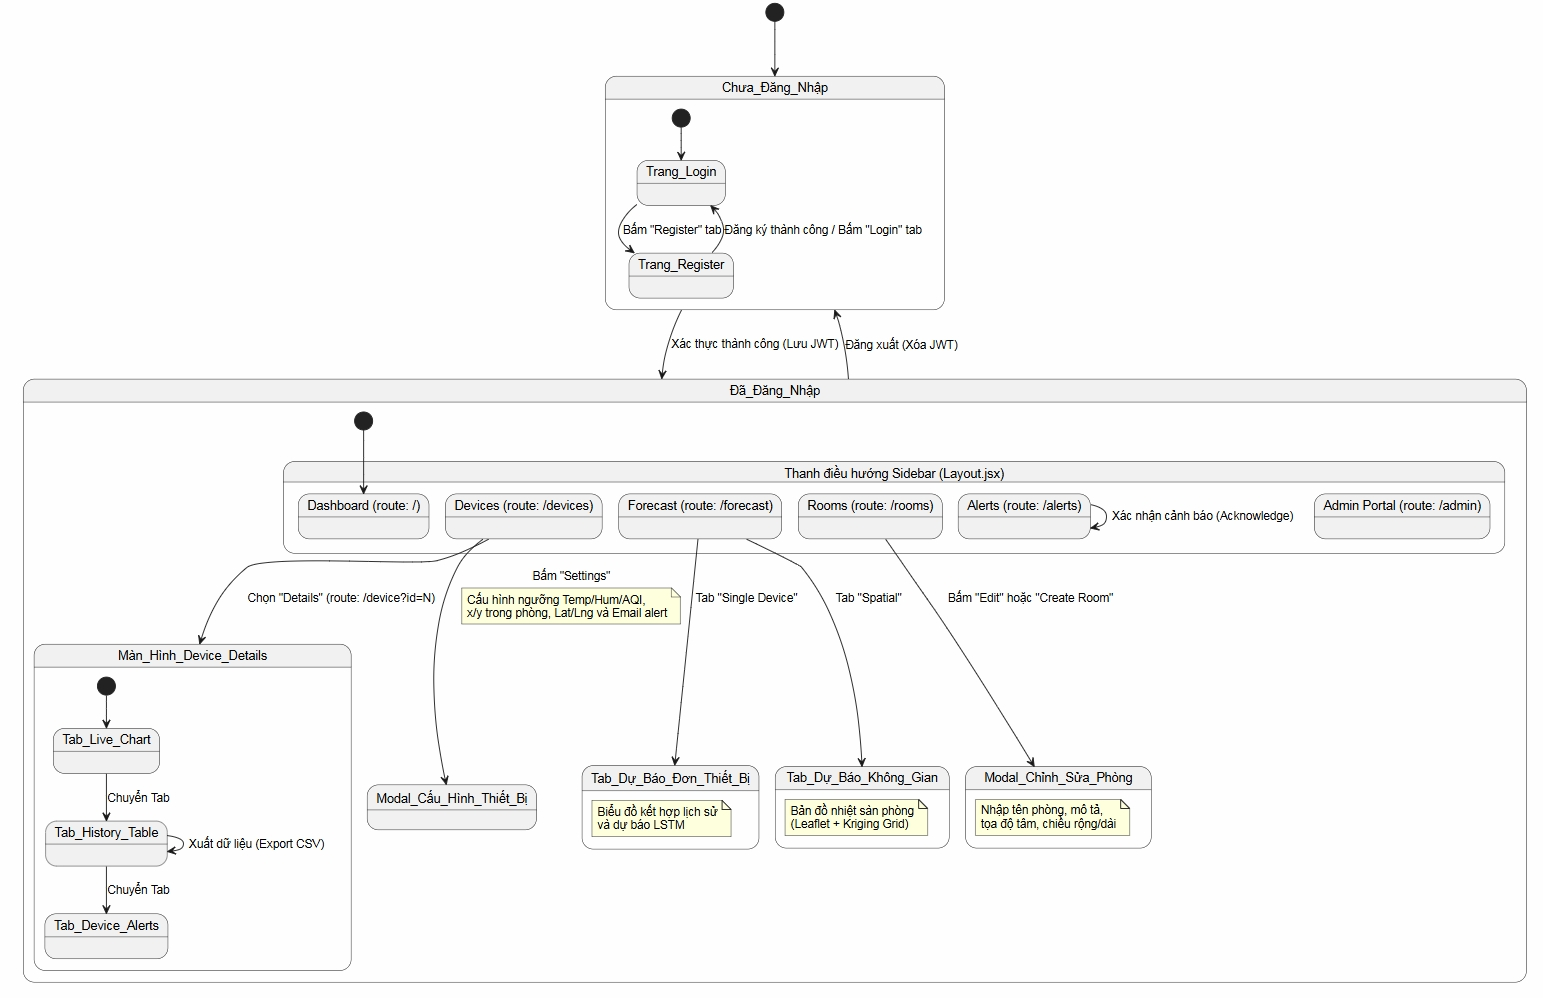
\includegraphics[width=0.85\textwidth]{nav_diagram}
  \caption{Sơ đồ điều hướng các trang trong React dashboard}
  \label{fig:nav_diagram}
\end{figure}

Các trang chức năng bao gồm:
\begin{itemize}[leftmargin=2cm]
  \item \textbf{Dashboard (Trang chủ):} Hiển thị danh sách tóm tắt thiết bị, cảnh báo gần nhất, biểu đồ cập nhật trực tiếp dữ liệu đo đạc (realtime line chart).
  \item \textbf{Thiết bị (Devices):} Danh sách chi tiết các node cảm biến, cho phép thay đổi cấu hình ngưỡng cảnh báo và xem lại dữ liệu lịch sử.
  \item \textbf{Dự báo (Forecast):} Tab dự báo trạm (Single Device) hiển thị biểu đồ dự báo LSTM tương lai và Tab dự báo không gian (Spatial) hiển thị heatmap nội suy không gian của căn phòng được chọn.
  \item \textbf{Quản lý phòng (Rooms):} Nơi người quản trị tạo sơ đồ phòng học, định vị toạ độ $x, y$ đặt các thiết bị trên mặt bằng sàn.
  \item \textbf{Cảnh báo (Alerts):} Danh sách lịch sử các cảnh báo kèm chức năng xác nhận đã xử lý (acknowledge).
\end{itemize}

%------------------------------------------------------------
\section{Triển khai}
\label{sec:design:deploy}
%------------------------------------------------------------

\subsection{Môi trường triển khai}
\label{subsec:design:deploy:env}

Hệ thống được triển khai và kiểm thử trong môi trường phòng lab với cấu hình cụ thể như sau:

\begin{table}[H]
  \centering
  \caption{Cấu hình môi trường triển khai}
  \label{tab:deploy_env}
  \begin{tabular}{ll}
    \toprule
    \textbf{Thành phần} & \textbf{Cấu hình} \\
    \midrule
    Máy chủ Backend     & Máy tính cá nhân / Laptop \\
    Hệ điều hành        & Ubuntu 22.04 LTS / Windows 11 (WSL2) \\
    Node.js             & v18 LTS \\
    Python              & 3.10+ \\
    PostgreSQL          & v15, chạy local \\
    Node IoT            & ESP32 DevKit v1 + DHT11 \\
    Mạng                & Wi-Fi LAN cùng subnet \\
    \bottomrule
  \end{tabular}
\end{table}

\subsection{Hướng dẫn khởi động hệ thống}
\label{subsec:design:deploy:guide}

Quy trình khởi động hệ thống theo thứ tự:

\begin{enumerate}[leftmargin=2cm]
  \item \textbf{Khởi động cơ sở dữ liệu PostgreSQL} và thực thi các câu lệnh SQL khởi tạo cấu trúc bảng từ tệp \texttt{schema.sql} (chi tiết xem tại Phụ lục~\ref{lst:schema}).
  \item \textbf{Khởi động Backend Node.js:}
    Di chuyển vào thư mục \texttt{server/}, cài đặt các gói thư viện phụ thuộc bằng lệnh \texttt{npm install}, tạo tệp cấu hình biến môi trường \texttt{.env} chứa thông tin kết nối PostgreSQL, khóa bí mật JWT\_SECRET, và thông tin SMTP email cảnh báo. Cuối cùng khởi chạy máy chủ bằng lệnh \texttt{node index.js}.
  \item \textbf{Khởi động hai FastAPI Machine Learning service (chạy đồng thời):}
    Di chuyển vào thư mục \texttt{forecast/}. Khởi chạy service dự báo chuỗi thời gian LSTM ở cổng \texttt{8000} bằng lệnh:
    \texttt{uvicorn time\_forecast.main:app --port 8000 --reload}.
    Khởi chạy service nội suy không gian địa thống kê Kriging ở cổng \texttt{8001} bằng lệnh:
    \texttt{uvicorn spatial\_forecast:app --port 8001 --reload}.
  \item \textbf{Khởi động Frontend React:}
    Di chuyển vào thư mục \texttt{frontend/}, chạy lệnh \texttt{npm install} để cài đặt các thư viện React. Khởi chạy máy chủ phát triển frontend ở chế độ Local Development bằng lệnh \texttt{npm run dev} (mặc định chạy ở cổng \texttt{5173}).
  \item \textbf{Nạp firmware lên ESP32:}
    Mở file \texttt{sensor/sensor.ino} trên môi trường phát triển Arduino IDE. Cập nhật các hằng số Wi-Fi SSID, mật khẩu mạng Wi-Fi và địa chỉ IP tĩnh của máy chủ backend làm MQTT Broker. Thực hiện biên dịch và nạp chương trình lên vi điều khiển ESP32 qua cáp micro-USB.
  \item \textbf{Kiểm thử giao diện:}
    Mở trình duyệt web truy cập địa chỉ \texttt{http://localhost:5173}. Đăng ký tài khoản người dùng đầu tiên để đăng nhập vào Dashboard. Bật nguồn node cảm biến ESP32, thiết bị sẽ tự động đăng ký và truyền dữ liệu cập nhật tức thời lên giao diện biểu đồ realtime của hệ thống.
\end{enumerate}

\subsection{Script mô phỏng node IoT}
\label{subsec:design:deploy:simulate}

Để phục vụ việc kiểm thử khả năng chịu tải, luồng dữ liệu truyền tải của nhiều thiết bị đo cùng lúc mà không cần phần cứng thực tế, đồ án cung cấp một script mô phỏng chạy bằng Node.js. Thuật toán của script mô phỏng được mô tả bằng mã giả như sau:

\begin{lstlisting}[language=JavaScript, caption={Giai thuat script mo phong node thiet bi gui du lieu len may chu}, label={lst:simulate_pseudo}]
Ham moPhongGuiDuLieu()
    Ket noi toi dia chi MQTT Broker noi bo ("mqtt://localhost:1883")
    Dat ma API_KEY = "your-api-key-here" (ma khoa xac thuc da dang ky trong DB)
    Dinh ky moi 5 giay thuc hien:
        nhietDo = Sinh so thuc ngau nhien tu 20.0 den 35.0 (lay 1 chu so thap phan)
        doAm = Sinh so thuc ngau nhien tu 40.0 den 80.0
        aqi = Sinh so thuc ngau nhien tu 30.0 den 100.0 (chi so chat luong khong khi gia lap)
        goiTin = Dong goi JSON { "temperature": nhietDo, "humidity": doAm, "aqi": aqi }
        Publish goi tin len topic "device/" + API_KEY + "/data"
        In thong tin log ra man hinh console
Ket thuc Ham
\end{lstlisting}

%------------------------------------------------------------
\section{Tổng hợp công nghệ sử dụng trong hệ thống}
\label{sec:design:tech_summary}
%------------------------------------------------------------

Bảng~\ref{tab:tech_summary} tổng hợp toàn bộ các công nghệ cốt lõi được lựa chọn sử dụng xuyên suốt các thành phần của hệ thống cùng với các lý do kỹ thuật tương ứng.

\begin{table}[H]
  \centering
  \caption{Tổng hợp công nghệ sử dụng trong hệ thống}
  \label{tab:tech_summary}
  \begin{tabularx}{\textwidth}{p{3cm} p{3.2cm} X}
    \toprule
    \textbf{Thành phần} & \textbf{Công nghệ} & \textbf{Lý do lựa chọn} \\
    \midrule
    Vi điều khiển
      & ESP32
      & Tích hợp Wi-Fi, chi phí thấp, hiệu năng xử lý cao, hệ sinh thái phong phú \\
    Cảm biến
      & DHT11
      & Giao tiếp đơn giản 1-Wire, chi phí cực thấp, đủ chính xác cho prototype \\
    Giao thức IoT
      & MQTT (Aedes)
      & Gói tin nhẹ, overhead tối thiểu, kết nối TCP bền vững, tích hợp Node.js \\
    Backend chính
      & Node.js/Express
      & Xử lý bất đồng bộ I/O tốt, điều phối nhiều kết nối realtime đồng thời \\
    Realtime push
      & Socket.io
      & Thiết lập WebSocket hai chiều nhanh, quản lý room theo thiết bị hiệu quả \\
    Cơ sở dữ liệu
      & PostgreSQL
      & Hệ quản trị quan hệ bền vững, truy vấn nhanh chuỗi thời gian nhờ lập chỉ mục \\
    ML Framework
      & PyTorch
      & Hỗ trợ đồ thị tính toán động, dễ xây dựng và lưu model weights cho suy luận \\
    ML Service
      & FastAPI (Python)
      & Lập trình async Python API hiệu năng cao, tự sinh OpenAPI docs tiện lợi \\
    Nội suy không gian
      & Kriging / IDW
      & Kriging tối ưu phương sai nội suy mịn, IDW bổ trợ góc biên phòng \\
    Frontend
      & React 19 + Vite
      & UI dạng component dễ bảo trì, Vite HMR cập nhật tức thời khi dev \\
    Biểu đồ
      & Chart.js
      & Dung lượng nhẹ, hỗ trợ render động khi có dữ liệu mới qua WebSockets \\
    Bản đồ mặt bằng
      & Leaflet
      & Thư viện bản đồ tương tác mã nguồn mở nhẹ, dễ vẽ lớp heatmap tùy biến \\
    \bottomrule
  \end{tabularx}
\end{table}

%============================================================
% CHƯƠNG 4: THIẾT KẾ, TRIỂN KHAI VÀ ĐÁNH GIÁ HỆ THỐNG
%============================================================
\chapter{THIẾT KẾ, TRIỂN KHAI VÀ ĐÁNH GIÁ HỆ THỐNG}
\label{chap:design}

Chương này trình bày toàn bộ quá trình thiết kế và xây dựng hệ thống
AIoT giám sát và dự báo chất lượng không khí. Nội dung bao gồm thiết
kế kiến trúc tổng thể theo mô hình bốn tầng, thiết kế chi tiết từng
thành phần (phần cứng, firmware, backend, ML pipeline, cơ sở dữ liệu,
dashboard), kết quả xây dựng và kiểm thử, cùng thông tin triển khai
thực tế.

%------------------------------------------------------------
\section{Thiết kế kiến trúc}
\label{sec:design:arch}
%------------------------------------------------------------

\subsection{Lựa chọn kiến trúc phần mềm}
\label{subsec:design:arch:choice}

Hệ thống được thiết kế theo \textbf{kiến trúc bốn tầng} kết hợp mô
hình IoT Gateway, thể hiện trong Hình~\ref{fig:arch_overview}. Kiến
trúc này phân tách rõ ràng trách nhiệm của từng tầng, đảm bảo khả năng
mở rộng độc lập và dễ bảo trì:

\begin{enumerate}[leftmargin=2cm]
  \item \textbf{Tầng thu thập (Edge Layer):} Node cảm biến ESP32/DHT11
    đọc dữ liệu và gửi lên qua MQTT. Tầng này hoạt động hoàn toàn
    tự động, không cần can thiệp người dùng sau khi cấu hình ban đầu.
  \item \textbf{Tầng truyền dẫn (Transport Layer):} Giao thức MQTT
    với Aedes broker tích hợp trong Node.js, đảm bảo truyền dữ liệu
    nhẹ, độ trễ thấp và hỗ trợ many node đồng thời.
  \item \textbf{Tầng xử lý và lưu trữ (Backend Layer):} Node.js/Express
    xử lý nghiệp vụ, PostgreSQL lưu trữ dữ liệu chuỗi thời gian,
    FastAPI/PyTorch chạy LSTM inference và nội suy Kriging/IDW.
  \item \textbf{Tầng hiển thị (Presentation Layer):} React dashboard
    nhận dữ liệu realtime qua Socket.io, hiển thị biểu đồ Chart.js
    và heatmap Leaflet.
\end{enumerate}

\begin{figure}[H]
  \centering
  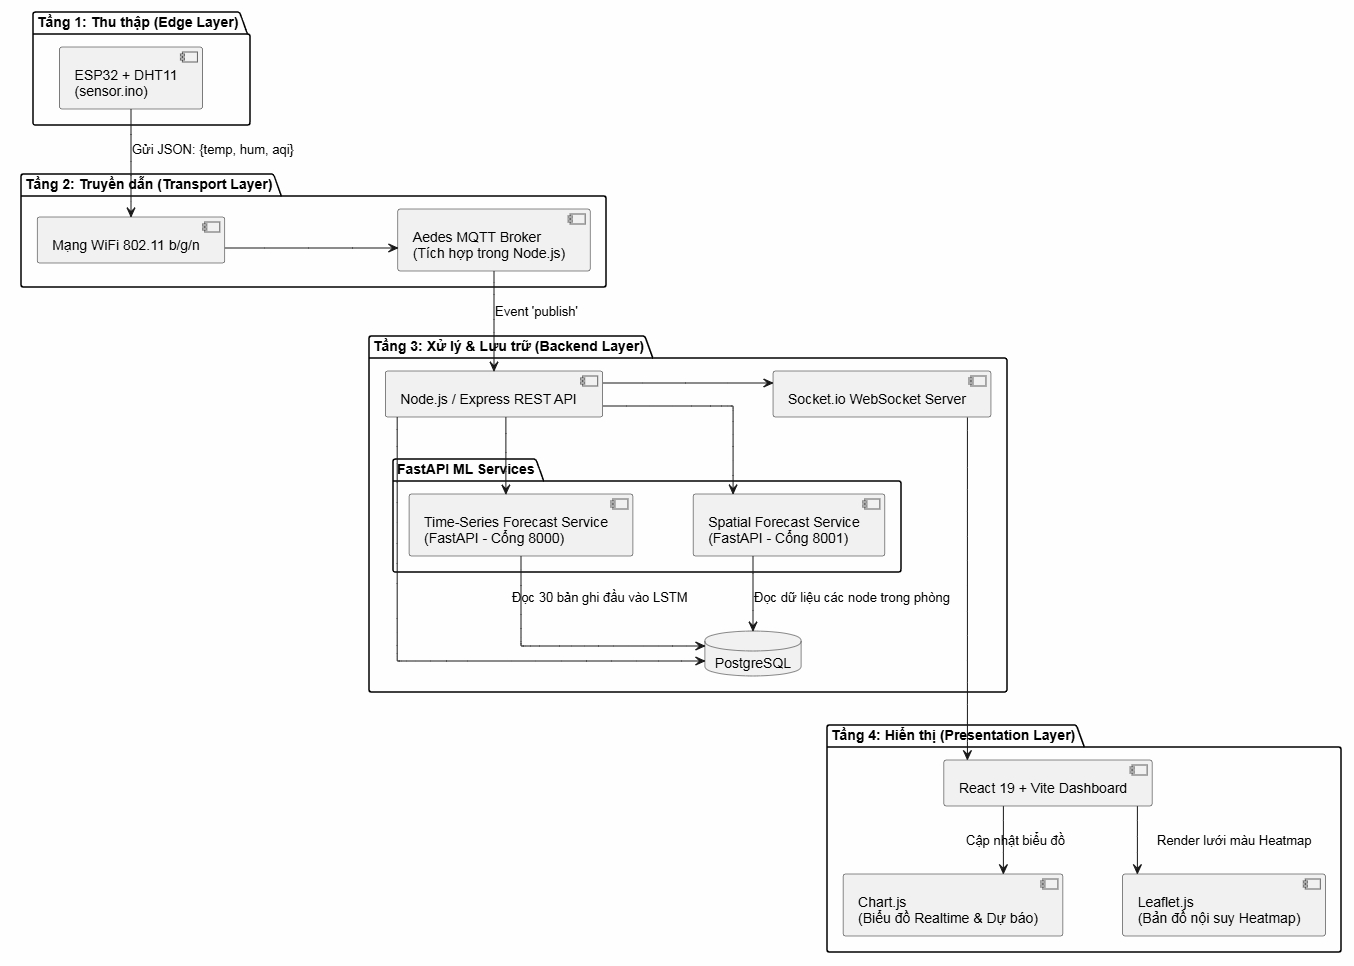
\includegraphics[width=0.95\textwidth]{arch_overview}
  \caption{Kiến trúc tổng quan của hệ thống AIoT giám sát và dự báo
  chất lượng không khí}
  \label{fig:arch_overview}
\end{figure}

Lý do lựa chọn kiến trúc này so với các phương án khác:

\begin{itemize}[leftmargin=2cm]
  \item \textbf{So với kiến trúc monolithic:} Việc tách FastAPI ML
    service khỏi Node.js backend cho phép mỗi service scale độc lập
    và tránh block event loop khi chạy inference nặng.
  \item \textbf{So với kiến trúc serverless:} Hệ thống cần duy trì
    kết nối MQTT và WebSocket liên tục, không phù hợp với mô hình
    serverless stateless.
  \item \textbf{So với Cloud-only:} Aedes broker tích hợp trong
    Node.js giảm một hop mạng (không cần Mosquitto riêng), giảm độ
    trễ và đơn giản hóa triển khai.
\end{itemize}

\subsection{Thiết kế tổng quan các gói}
\label{subsec:design:arch:packages}

Hình~\ref{fig:package_diagram} mô tả biểu đồ phụ thuộc gói tổng quan
của hệ thống, phân chia thành bốn nhóm chính tương ứng với bốn tầng
kiến trúc.

\begin{figure}[H]
  \centering
  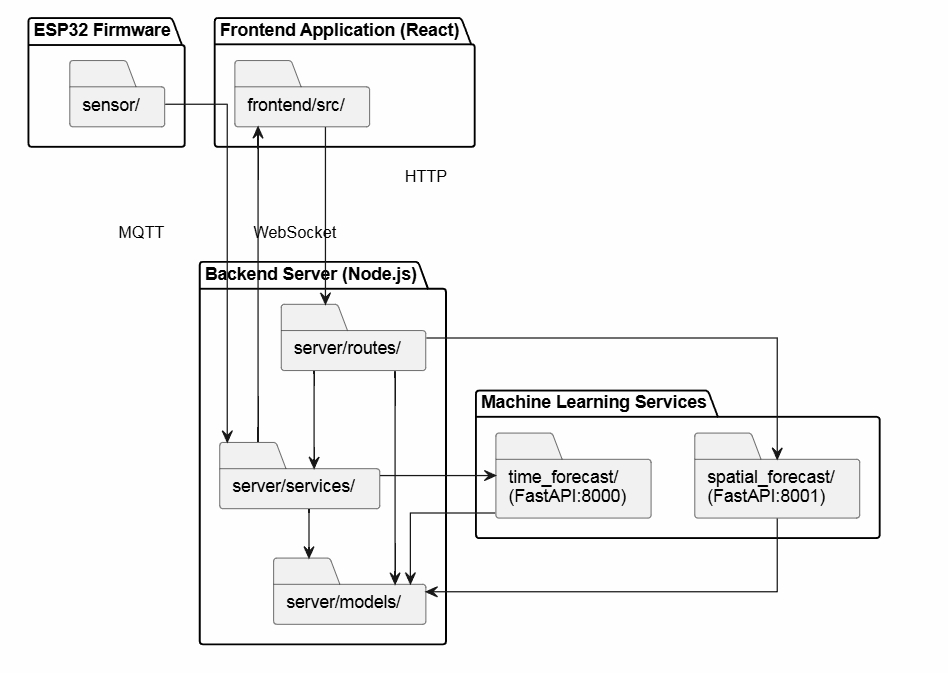
\includegraphics[width=0.95\textwidth]{package_diagram}
  \caption{Biểu đồ phụ thuộc gói tổng quan của hệ thống}
  \label{fig:package_diagram}
\end{figure}

Cấu trúc thư mục dự án phản ánh trực tiếp kiến trúc này:

\begin{itemize}[leftmargin=2cm]
  \item \texttt{sensor/} - Firmware ESP32 (Arduino/C++)
  \item \texttt{server/} - Backend Node.js/Express
    \begin{itemize}
      \item \texttt{controllers/} - Xử lý HTTP request
      \item \texttt{routes/} - Định nghĩa API endpoint
      \item \texttt{services/} - Logic nghiệp vụ
        (alertService, mqttService, forecastService)
      \item \texttt{middleware/} - Xác thực JWT, phân quyền
      \item \texttt{models/} - Kết nối PostgreSQL
    \end{itemize}
  \item \texttt{lstm\_train/} - Python ML pipeline
    (train, inference, spatial\_forecast FastAPI)
  \item \texttt{frontend/src/} - React dashboard
    \begin{itemize}
      \item \texttt{pages/} - Các trang chính
      \item \texttt{components/} - UI components
      \item \texttt{context/} - React Context quản lý
        trạng thái toàn cục
    \end{itemize}
\end{itemize}

%------------------------------------------------------------
\section{Thiết kế chi tiết}
\label{sec:design:detail}
%------------------------------------------------------------

\subsection{Thiết kế phần cứng node cảm biến}
\label{subsec:design:hardware}

\subsubsection*{a. Sơ đồ kết nối phần cứng}

Node cảm biến được xây dựng từ hai thành phần chính: vi điều khiển
ESP32 và cảm biến DHT11. Sơ đồ kết nối được thể hiện trong
Hình~\ref{fig:hardware_schematic}.

\begin{figure}[H]
  \centering
  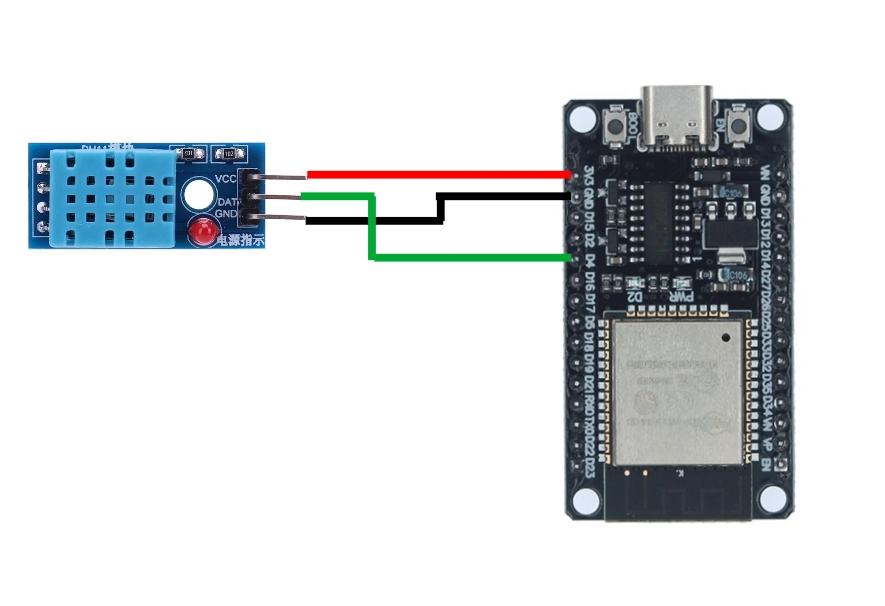
\includegraphics[width=0.7\textwidth]{hardware_schematic}
  \caption{Sơ đồ kết nối phần cứng node cảm biến}
  \label{fig:hardware_schematic}
\end{figure}

Bảng~\ref{tab:gpio_config} liệt kê cấu hình chân kết nối:

\begin{table}[H]
  \centering
  \caption{Cấu hình chân kết nối ESP32 --- DHT11}
  \label{tab:gpio_config}
  \begin{tabular}{llll}
    \toprule
    \textbf{Chân DHT11} & \textbf{Chân ESP32} & \textbf{Chức năng}
      & \textbf{Ghi chú} \\
    \midrule
    VCC  & 3.3V   & Nguồn cấp      & --- \\
    DATA & GPIO4  & Dữ liệu 1-Wire & Qua điện trở 10k$\Omega$ pull-up \\
    GND  & GND    & Nối đất        & --- \\
    \bottomrule
  \end{tabular}
\end{table}

\subsubsection*{b. Cơ chế lưu cấu hình trên Flash}

Mỗi node cần lưu trữ \texttt{api\_key} và cấu hình nhận được từ
backend qua các lần reset. ESP32 sử dụng thư viện
\texttt{Preferences.h} để ghi vào vùng NVS (Non-Volatile Storage)
của Flash:

\begin{lstlisting}[language=C, caption={Lưu và đọc cấu hình định danh từ Flash ESP32}, label={lst:preferences}]
#include <Preferences.h>
Preferences prefs;

// Đọc device_id và api_key từ NVS Flash khi khởi động
void loadCredentials() {
    prefs.begin("device", true);       // namespace "device", read-only
    deviceId     = prefs.getInt(   "device_id", -1);
    deviceApiKey = prefs.getString("api_key",  "");
    prefs.end();
}

// Ghi device_id và api_key sau khi nhận từ backend qua MQTT
void saveCredentials(int newId, String newKey) {
    prefs.begin("device", false);      // read-write
    prefs.putInt(   "device_id", newId);
    prefs.putString("api_key",   newKey);
    prefs.end();
}
// Lưu ý: logic so sánh ngưỡng cảnh báo (temp_high, hum_low...)
// được thực hiện tập trung ở Backend Node.js (alertService.js),
// không lưu trên firmware để giảm tải cho vi điều khiển.
\end{lstlisting}

\subsection{Thiết kế Firmware}
\label{subsec:design:firmware}

\subsubsection*{a. Kiến trúc firmware phân tầng}

Firmware được tổ chức theo kiến trúc phân tầng như minh họa trong
Hình~\ref{fig:firmware_arch}. Vòng lặp chính (\texttt{loop()}) điều
phối ba tác vụ theo chu kỳ: đọc cảm biến, duy trì kết nối MQTT và
gửi dữ liệu.

\begin{figure}[H]
  \centering
  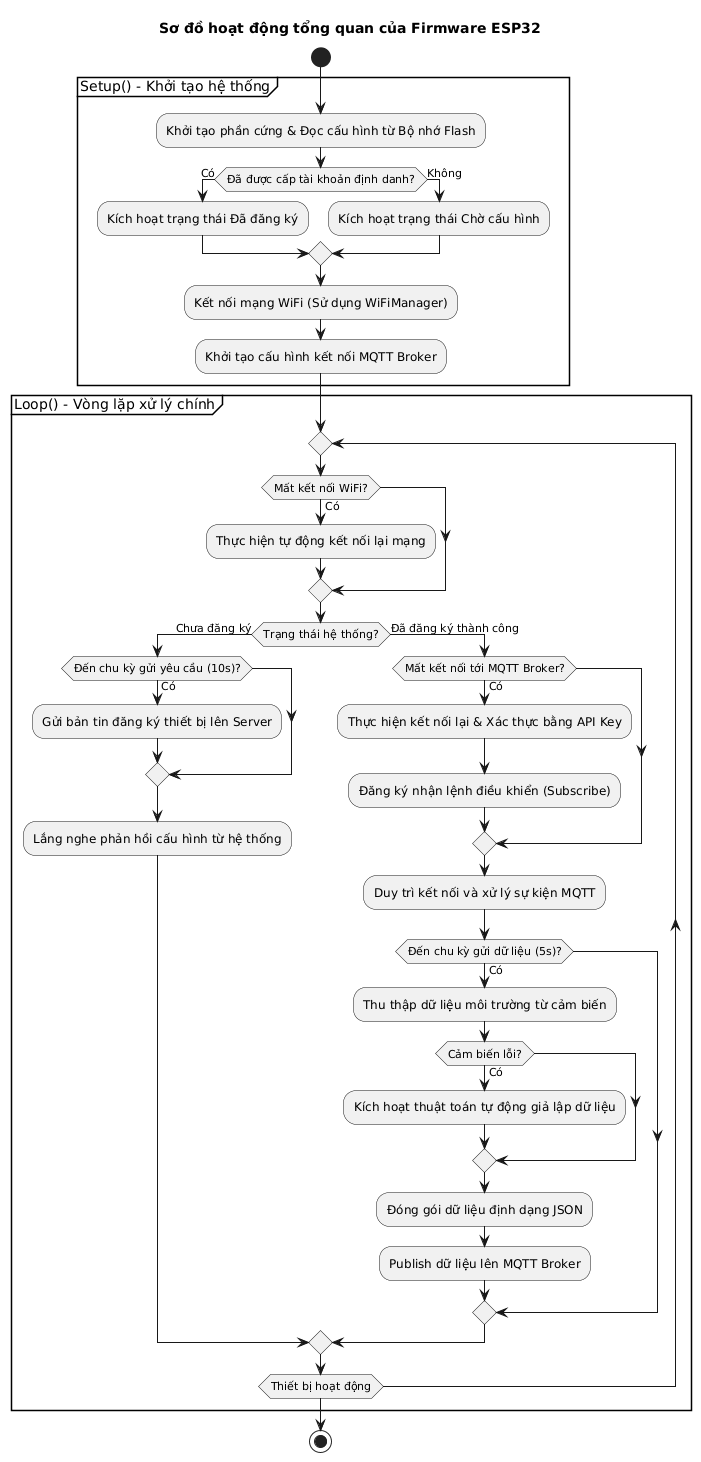
\includegraphics[width=0.75\textwidth]{firmware_arch}
  \caption{Kiến trúc firmware phân tầng của node ESP32}
  \label{fig:firmware_arch}
\end{figure}

\subsubsection*{b. Luồng xử lý chính của firmware}

\begin{lstlisting}[language=C, caption={Luồng chính firmware ESP32},
label={lst:firmware_main}]
#include <WiFi.h>
#include <PubSubClient.h>
#include <ArduinoJson.h>
#include <DHT.h>
#include <Preferences.h>
#include <WiFiManager.h>

#define DHTPIN 4
#define DHTTYPE DHT11
#define SEND_INTERVAL 5000   // 5 giay

DHT dht(DHTPIN, DHTTYPE);
WiFiClient wifiClient;
PubSubClient mqttClient(wifiClient);

String deviceApiKey = "";
int    deviceId     = -1;
bool   provisioned  = false;

void setup() {
    dht.begin();
    loadCredentials();  // Doc device_id, api_key tu Flash
    WiFiManager wm;
    wm.autoConnect("Sensor-Setup-[MAC]");
    mqttClient.setServer(MQTT_BROKER, 1883);
    mqttClient.setCallback(mqttCallback);
}

void loop() {
    if (!provisioned) { sendProvisionRequest(); return; }
    if (!mqttClient.connected()) reconnectWithAuth();
    mqttClient.loop();

    // Gui du lieu theo chu ky SEND_INTERVAL
    if (millis() - lastSend >= SEND_INTERVAL) {
        float temp = dht.readTemperature();
        float hum  = dht.readHumidity();
        float aqi  = generateMockAqi(); // Giai lap AQI bang Box-Muller

        if (!isnan(temp) && !isnan(hum)) {
            publishData(temp, hum, aqi);
        }
        lastSend = millis();
    }
}

void publishData(float temp, float hum, float aqi) {
    StaticJsonDocument<128> doc;
    doc["temperature"] = temp;
    doc["humidity"]    = hum;
    doc["aqi"]         = aqi;  // bat buoc cho ML pipeline
    char payload[128];
    serializeJson(doc, payload);

    String topic = "device/" + deviceApiKey + "/data";
    mqttClient.publish(topic.c_str(), payload);
}
\end{lstlisting}

\subsubsection*{c. Xử lý message cấu hình từ backend}

Khi nhận cấu hình từ topic \texttt{devices/\{mac\}/config}, callback
MQTT lưu thông tin định danh thiết bị vào Flash và đặt cờ
\texttt{provisioned} để chuyển sang chế độ gửi dữ liệu:

\begin{lstlisting}[language=C, caption={Callback xử lý message cấu
hình MQTT}, label={lst:mqtt_callback}]
void mqttCallback(char* topic, byte* payload,
                  unsigned int length) {
    StaticJsonDocument<256> doc;
    deserializeJson(doc, payload, length);

    // Xu ly lenh reset tu backend (xoa flash, restart)
    if (doc["action"] == "reset") {
        prefs.begin("device", false);
        prefs.clear(); prefs.end();
        ESP.restart(); return;
    }

    // Nhan device_id va api_key tu backend provisioning
    if (doc.containsKey("device_id") &&
        doc.containsKey("api_key")) {
        int    newId  = doc["device_id"].as<int>();
        String newKey = doc["api_key"].as<String>();
        saveCredentials(newId, newKey);
        deviceId     = newId;
        deviceApiKey = newKey;
        provisioned  = true;
    }
    // Logic kiem tra nguong canh bao (temp_high, hum_low...)
    // duoc xu ly tap trung tai alertService.js phia Backend,
    // khong can luu tren firmware.
}
\end{lstlisting}

\subsection{Thiết kế cơ sở dữ liệu}
\label{subsec:design:database}

\subsubsection*{a. Sơ đồ ERD}

Cơ sở dữ liệu PostgreSQL gồm 5 bảng chính, quan hệ được thể hiện
trong Hình~\ref{fig:erd}.

\begin{figure}[H]
  \centering
  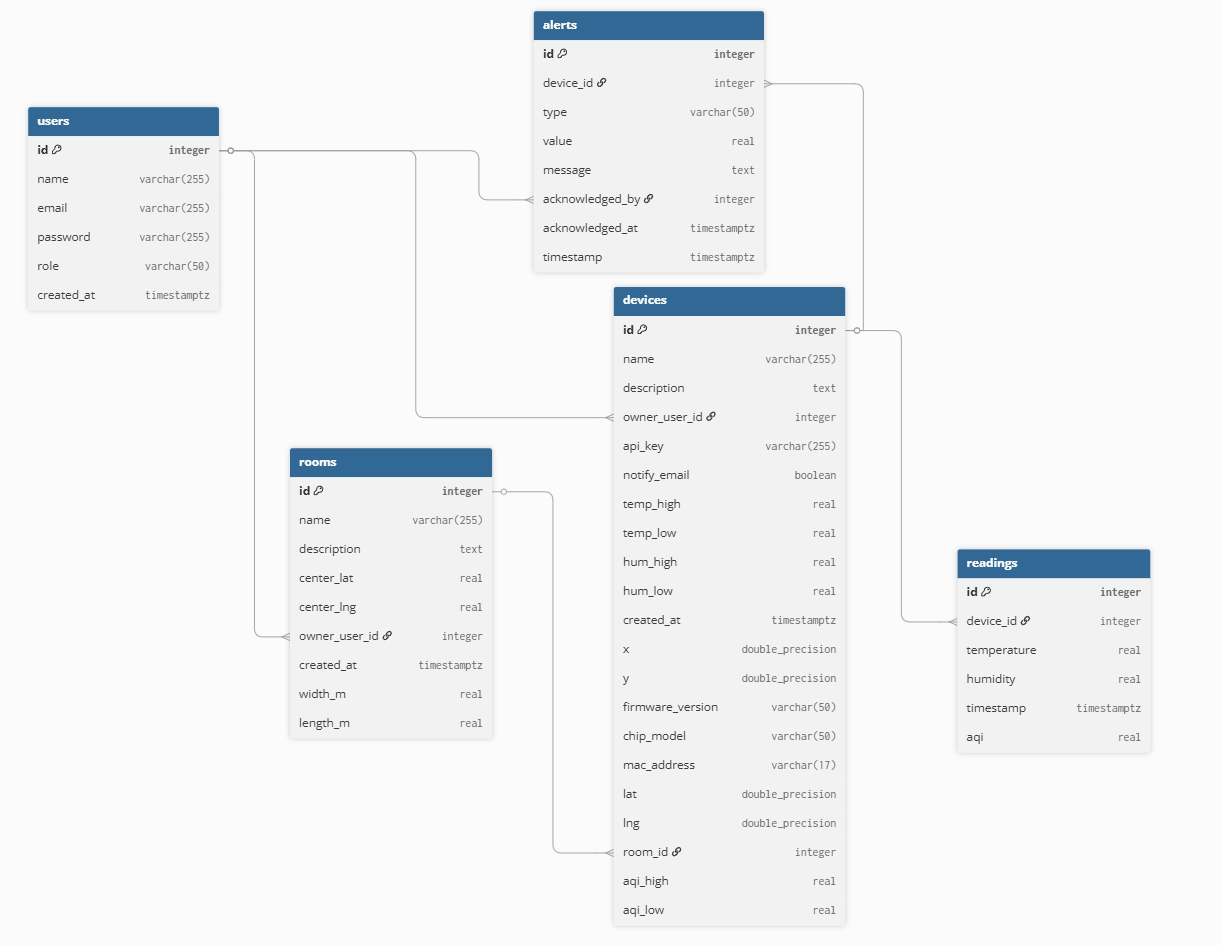
\includegraphics[width=\textwidth]{erd}
  \caption{Sơ đồ ERD cơ sở dữ liệu PostgreSQL}
  \label{fig:erd}
\end{figure}

\subsubsection*{b. Định nghĩa schema}

\begin{lstlisting}[language=SQL, caption={Schema cơ sở dữ liệu
PostgreSQL}, label={lst:schema}]
-- Bang nguoi dung
CREATE TABLE users (
    id         SERIAL PRIMARY KEY,
    name       VARCHAR(100),
    email      VARCHAR(100) UNIQUE NOT NULL,
    password   VARCHAR(255) NOT NULL,    -- bcrypt hash
    role       VARCHAR(20) DEFAULT 'user',
    created_at TIMESTAMP DEFAULT NOW()
);
-- Bang phong/khu vuc
CREATE TABLE rooms (
    id            SERIAL PRIMARY KEY,
    name          VARCHAR(100),
    description   TEXT,
    center_lat    REAL,       -- Toa do tam phong
    center_lng    REAL,
    width_m       REAL,       -- Kich thuoc(met)
    length_m      REAL,
    owner_user_id INTEGER REFERENCES users(id),
    created_at    TIMESTAMP DEFAULT NOW()
);
-- Bang thiet bi IoT
CREATE TABLE devices (
    id               SERIAL PRIMARY KEY,
    name             VARCHAR(100),
    description      TEXT,
    owner_user_id    INTEGER REFERENCES users(id),
    api_key          VARCHAR(64) UNIQUE NOT NULL,
    notify_email     BOOLEAN DEFAULT TRUE,
    temp_high        REAL DEFAULT 35.0,
    temp_low         REAL DEFAULT 10.0,
    hum_high         REAL DEFAULT 80.0,
    hum_low          REAL DEFAULT 20.0,
    aqi_high         REAL,
    aqi_low          REAL,
    room_id          INTEGER REFERENCES rooms(id),
    mac_address      VARCHAR(17) UNIQUE,  -- dia chi MAC cua ESP32
    x                DOUBLE PRECISION,   -- toa do X trong phong (m)
    y                DOUBLE PRECISION,   -- toa do Y trong phong (m)
    lat              DOUBLE PRECISION,   -- vi do thuc te (WGS84)
    lng              DOUBLE PRECISION,   -- kinh do thuc te (WGS84)
    firmware_version VARCHAR(50),
    chip_model       VARCHAR(50),
    created_at       TIMESTAMP DEFAULT NOW()
);
-- Bang du lieu cam bien
CREATE TABLE readings (
    id          SERIAL PRIMARY KEY,
    device_id   INTEGER REFERENCES devices(id),
    temperature REAL NOT NULL,
    humidity    REAL NOT NULL,
    aqi         REAL NOT NULL DEFAULT 0,  -- chi so chat luong KK
    timestamp   TIMESTAMP DEFAULT NOW()
);
-- Index tang toc truy van chuoi thoi gian
CREATE INDEX idx_readings_device_time
    ON readings(device_id, timestamp DESC);
-- Bang canh bao
CREATE TABLE alerts (
    id              SERIAL PRIMARY KEY,
    device_id       INTEGER REFERENCES devices(id),
    type            VARCHAR(50),   -- 'temp_high', 'hum_low', 'aqi_high'...
    value           REAL,          -- Gia tri vuot nguong
    message         TEXT,
    acknowledged_by INTEGER REFERENCES users(id),
    acknowledged_at TIMESTAMP,
    timestamp       TIMESTAMP DEFAULT NOW()
);
\end{lstlisting}

\subsubsection*{c. Mối quan hệ giữa các bảng}

\begin{itemize}[leftmargin=2cm]
  \item \texttt{users} $\to$ \texttt{devices}: Một người dùng có thể
    sở hữu nhiều thiết bị. Mỗi thiết bị thuộc một người dùng.
  \item \texttt{users} $\to$ \texttt{rooms}: Một người dùng có thể
    quản lý nhiều phòng.
  \item \texttt{rooms} $\to$ \texttt{devices}: Một phòng có thể chứa
    nhiều node cảm biến. Mỗi node được gán vào một phòng.
  \item \texttt{devices} $\to$ \texttt{readings}: Quan hệ một-nhiều,
    mỗi thiết bị sinh ra nhiều bản ghi theo thời gian.
  \item \texttt{devices} $\to$ \texttt{alerts}: Cảnh báo được tạo tự
    động khi dữ liệu của thiết bị vượt ngưỡng cài đặt.
\end{itemize}

\subsection{Thiết kế Backend API}
\label{subsec:design:backend}

\subsubsection*{a. Cấu trúc API endpoints}

Backend Node.js/Express cung cấp RESTful API với prefix
\texttt{/api}. Tất cả endpoint (trừ auth) yêu cầu JWT trong header
\texttt{Authorization: Bearer \{token\}}.

\begin{table}[H]
  \centering
  \caption{API endpoints quản lý xác thực và người dùng}
  \label{tab:api_auth}
  \begin{tabularx}{\textwidth}{p{1.5cm} p{5cm} X}
    \toprule
    \textbf{Method} & \textbf{Endpoint} & \textbf{Mô tả} \\
    \midrule
    POST & \texttt{/api/auth/register} & Đăng ký tài khoản mới \\
    POST & \texttt{/api/auth/login}    & Đăng nhập, nhận JWT \\
    GET  & \texttt{/api/users/me}      & Lấy thông tin người dùng hiện tại \\
    PUT  & \texttt{/api/users/me}      & Cập nhật thông tin cá nhân \\
    \bottomrule
  \end{tabularx}
\end{table}

\begin{table}[H]
  \centering
  \caption{API endpoints quản lý thiết bị và phòng}
  \label{tab:api_devices}
  \begin{tabularx}{\textwidth}{p{1.5cm} p{4.5cm} X}
    \toprule
    \textbf{Method} & \textbf{Endpoint} & \textbf{Mô tả} \\
    \midrule
    GET    & \texttt{/api/devices}         & Danh sách thiết bị của user \\
    POST   & \texttt{/api/devices}         & Tạo thiết bị mới (Admin) \\
    GET    & \texttt{/api/devices/:id}     & Chi tiết một thiết bị \\
    PUT    & \texttt{/api/devices/:id}     & Cập nhật cấu hình/ngưỡng \\
    DELETE & \texttt{/api/devices/:id}     & Xóa thiết bị \\
    GET    & \texttt{/api/rooms}           & Danh sách phòng \\
    POST   & \texttt{/api/rooms}           & Tạo phòng mới \\
    PUT    & \texttt{/api/rooms/:id}       & Cập nhật thông tin phòng \\
    \bottomrule
  \end{tabularx}
\end{table}

\begin{table}[H]
  \centering
  \caption{API endpoints dữ liệu cảm biến, dự báo và cảnh báo}
  \label{tab:api_data}
  \begin{tabularx}{\textwidth}{p{1.5cm} p{5cm} X}
    \toprule
    \textbf{Method} & \textbf{Endpoint} & \textbf{Mô tả} \\
    \midrule
    GET & \texttt{/api/data}              & Lịch sử dữ liệu theo \texttt{device\_id}, \texttt{start}, \texttt{end} \\
    GET & \texttt{/api/forecast}          & Gọi FastAPI LSTM, trả về 15 giá trị dự báo \\
    GET & \texttt{/api/spatial-forecast}  & Gọi FastAPI Kriging, trả về lưới 40$\times$50 \\
    GET & \texttt{/api/alerts}            & Danh sách cảnh báo (lọc theo device, thời gian) \\
    PUT & \texttt{/api/alerts/:id/ack}    & Xác nhận (acknowledge) một cảnh báo \\
    \bottomrule
  \end{tabularx}
\end{table}

\subsubsection*{b. Cơ chế xác thực JWT}

\begin{lstlisting}[language=JavaScript, caption={Middleware xác thực
JWT}, label={lst:jwt_middleware}]
// middleware/auth.js
const jwt = require('jsonwebtoken');
module.exports = (req, res, next) => {
    const authHeader = req.headers['authorization'];
    if (!authHeader) return res.status(401)
        .json({ error: 'Missing token' });
    const token = authHeader.split(' ')[1]; // Bearer <token>
    try {
        const decoded = jwt.verify(token, process.env.JWT_SECRET);
        req.user = decoded;   // { id, email, role }
        next();
    } catch (err) {
        return res.status(403).json({ error: 'Invalid token' });
    }
};
\end{lstlisting}

\subsubsection*{c. Dịch vụ cảnh báo (alertService)}

\begin{lstlisting}[language=JavaScript, caption={Logic kiem tra nguong canh bao}, label={lst:alert_service}]
// services/alertService.js
async function check(device, reading) {
    const { temperature, humidity } = reading;
    const alerts = [];

    if (temperature > device.temp_high)
        alerts.push({ type: 'temp_high', value: temperature,
            message: `Nhiet do ${temperature}C vuot nguong ${device.temp_high}C` });
            
    if (temperature < device.temp_low)
        alerts.push({ type: 'temp_low', value: temperature,
            message: `Nhiet do ${temperature}C duoi nguong ${device.temp_low}C` });
            
    if (humidity > device.hum_high)
        alerts.push({ type: 'hum_high', value: humidity,
            message: `Do am ${humidity}% vuot nguong ${device.hum_high}%` });
            
    if (humidity < device.hum_low)
        alerts.push({ type: 'hum_low', value: humidity,
            message: `Do am ${humidity}% duoi nguong ${device.hum_low}%` });
            
    for (const alert of alerts) {
        // Luu vao DB
        await db.query(
            `INSERT INTO alerts
             (device_id, type, value, message, timestamp)
             VALUES ($1,$2,$3,$4,NOW())`,
            [device.id, alert.type,
             alert.value, alert.message]);
             
        // Gui email neu thiet bi bat notify
        if (device.notify_email)
            await emailService.sendAlert(device, alert);
    }
}
\end{lstlisting}

\subsection{Thiết kế và huấn luyện mô hình Machine Learning}
\label{subsec:design:ml}

\subsubsection*{a. Chuẩn bị dữ liệu}

Dữ liệu huấn luyện được thu thập từ hệ thống trong quá trình vận hành
thử nghiệm, lưu trữ trong bảng \texttt{readings}. Quy trình chuẩn bị
dữ liệu gồm các bước:

\begin{enumerate}[leftmargin=2cm]
  \item \textbf{Truy vấn:} Lấy toàn bộ dữ liệu từ PostgreSQL theo
    thứ tự thời gian tăng dần.
  \item \textbf{Kiểm tra missing values:} Bỏ qua các bản ghi có giá
    trị \texttt{NULL} hoặc nằm ngoài dải hợp lệ (nhiệt độ: $-10$ đến
    $60^\circ$C, độ ẩm: $0$ đến $100$\%).
  \item \textbf{Chuẩn hóa:} Áp dụng \texttt{MinMaxScaler}
    (scikit-learn) để đưa tất cả giá trị về khoảng $[0, 1]$. Lưu
    scaler vào \texttt{scaler.pkl} để tái dùng khi inference.
  \item \textbf{Tạo chuỗi (sliding window):} Với mỗi vị trí $t$,
    tạo cặp $(X_t, y_t)$ trong đó $X_t$ là ma trận $30 \times 3$
    (30 bước quá khứ, 3 features: nhiệt độ, độ ẩm, AQI) và $y_t$ là ma trận $15 \times 3$
    (15 bước tương lai cần dự báo).
  \item \textbf{Chia tập:} 80\% dữ liệu cho huấn luyện, 20\% cho
    kiểm thử.
\end{enumerate}

\subsubsection*{b. Kiến trúc mô hình LSTM}

Bảng~\ref{tab:lstm_arch} mô tả kiến trúc mô hình LSTM được sử dụng
trong đồ án.

\begin{table}[H]
  \centering
  \caption{Kiến trúc mô hình LSTM}
  \label{tab:lstm_arch}
  \begin{tabular}{lllr}
    \toprule
    \textbf{Layer} & \textbf{Loại} & \textbf{Tham số} &
    \textbf{Output shape} \\
    \midrule
    Input   & ---          & ---
      & $(batch, 30, 3)$ \\
    LSTM 1  & LSTM         & hidden=64, dropout=0.3
      & $(batch, 30, 64)$ \\
    LSTM 2  & LSTM         & hidden=64, dropout=0.3
      & $(batch, 64)$ \\
    Linear  & Fully connected & in=64, out=$15 \times 3$
      & $(batch, 45)$ \\
    Reshape & ---          & ---
      & $(batch, 15, 3)$ \\
    \bottomrule
    \multicolumn{3}{l}{\textit{Tổng số tham số:}}
      & \textit{$\approx$68.000} \\
  \end{tabular}
\end{table}

\subsubsection*{c. Huấn luyện và đánh giá}

Mô hình được huấn luyện với các siêu tham số:

\begin{table}[H]
  \centering
  \caption{Siêu tham số huấn luyện mô hình LSTM}
  \label{tab:lstm_hyperparams}
  \begin{tabular}{ll}
    \toprule
    \textbf{Siêu tham số} & \textbf{Giá trị} \\
    \midrule
    Optimizer      & Adam ($lr = 10^{-3}$) \\
    Loss function  & MSELoss \\
    Batch size     & 32 \\
    Số epoch tối đa& 100 \\
    Early stopping & patience = 10 epoch \\
    Dropout        & 0.3 (áp dụng giữa các LSTM layer) \\
    \bottomrule
  \end{tabular}
\end{table}

Kết quả huấn luyện thể hiện qua loss curve lưu tại
\texttt{lstm\_train/loss\_curve.png} (ngắn hạn) và
\texttt{loss\_curve\_long.png} (dài hạn). Đồ thị cho thấy training
loss và validation loss hội tụ ổn định, không có hiện tượng overfitting
rõ rệt nhờ cơ chế dropout và early stopping.

\subsection{Thiết kế Dashboard (Frontend)}
\label{subsec:design:frontend}

\subsubsection*{a. Sơ đồ điều hướng trang}

Hình~\ref{fig:nav_diagram} mô tả sơ đồ điều hướng giữa các trang
trong React dashboard. Trang Login là điểm vào bắt buộc; sau khi xác
thực thành công, người dùng được chuyển đến Dashboard chính.

\begin{figure}[H]
  \centering
  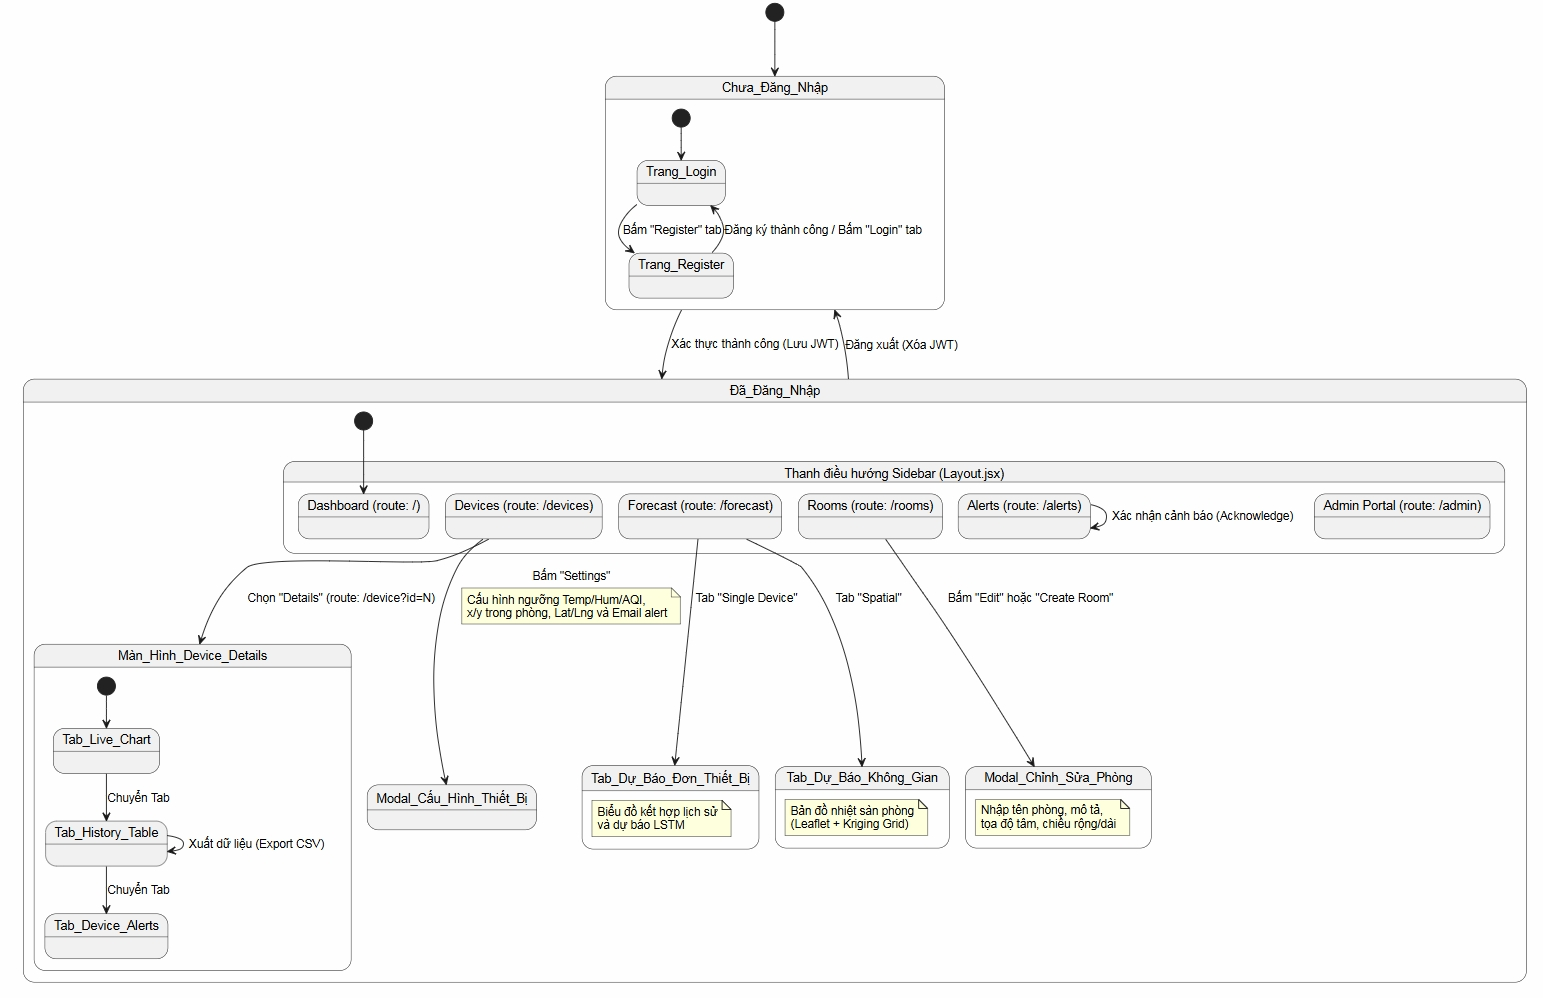
\includegraphics[width=0.85\textwidth]{nav_diagram}
  \caption{Sơ đồ điều hướng các trang trong React dashboard}
  \label{fig:nav_diagram}
\end{figure}

Các trang chính trong ứng dụng:

\begin{itemize}[leftmargin=2cm]
  \item \textbf{Login / Register:} Xác thực người dùng, lưu JWT vào
    localStorage.
  \item \textbf{Dashboard (trang chủ):} Hiển thị tổng quan tất cả
    node, biểu đồ realtime nhiệt độ, độ ẩm và AQI cập nhật qua Socket.io.
  \item \textbf{Trang thiết bị:} Danh sách node, cấu hình ngưỡng
    cảnh báo, xem biểu đồ lịch sử và dự báo LSTM cho từng node.
  \item \textbf{Trang dự báo (Forecast):} Gồm hai chế độ xem được
    chuyển đổi bằng tab: (1) \textbf{Single Device} --- biểu đồ dự
    báo chuỗi thời gian LSTM cho từng node theo các mốc 6/10/15 phút
    (ngắn hạn) và 1/3/6/12/24 giờ (dài hạn); (2) \textbf{Spatial} ---
    bản đồ heatmap Kriging/IDW phân bố môi trường không gian theo
    phòng, render trên Leaflet.
  \item \textbf{Trang cảnh báo:} Danh sách alert, bộ lọc theo thời
    gian, chức năng acknowledge.
  \item \textbf{Trang quản lý phòng:} Tạo và cấu hình phòng, gán
    node vào phòng, cài đặt tọa độ.
\end{itemize}

\subsubsection*{b. Thiết kế giao diện người dùng}

Hình~\ref{fig:ui_dashboard} và Hình~\ref{fig:ui_heatmap} minh họa
thiết kế giao diện của hai màn hình chính.

\begin{figure}[H]
  \centering
  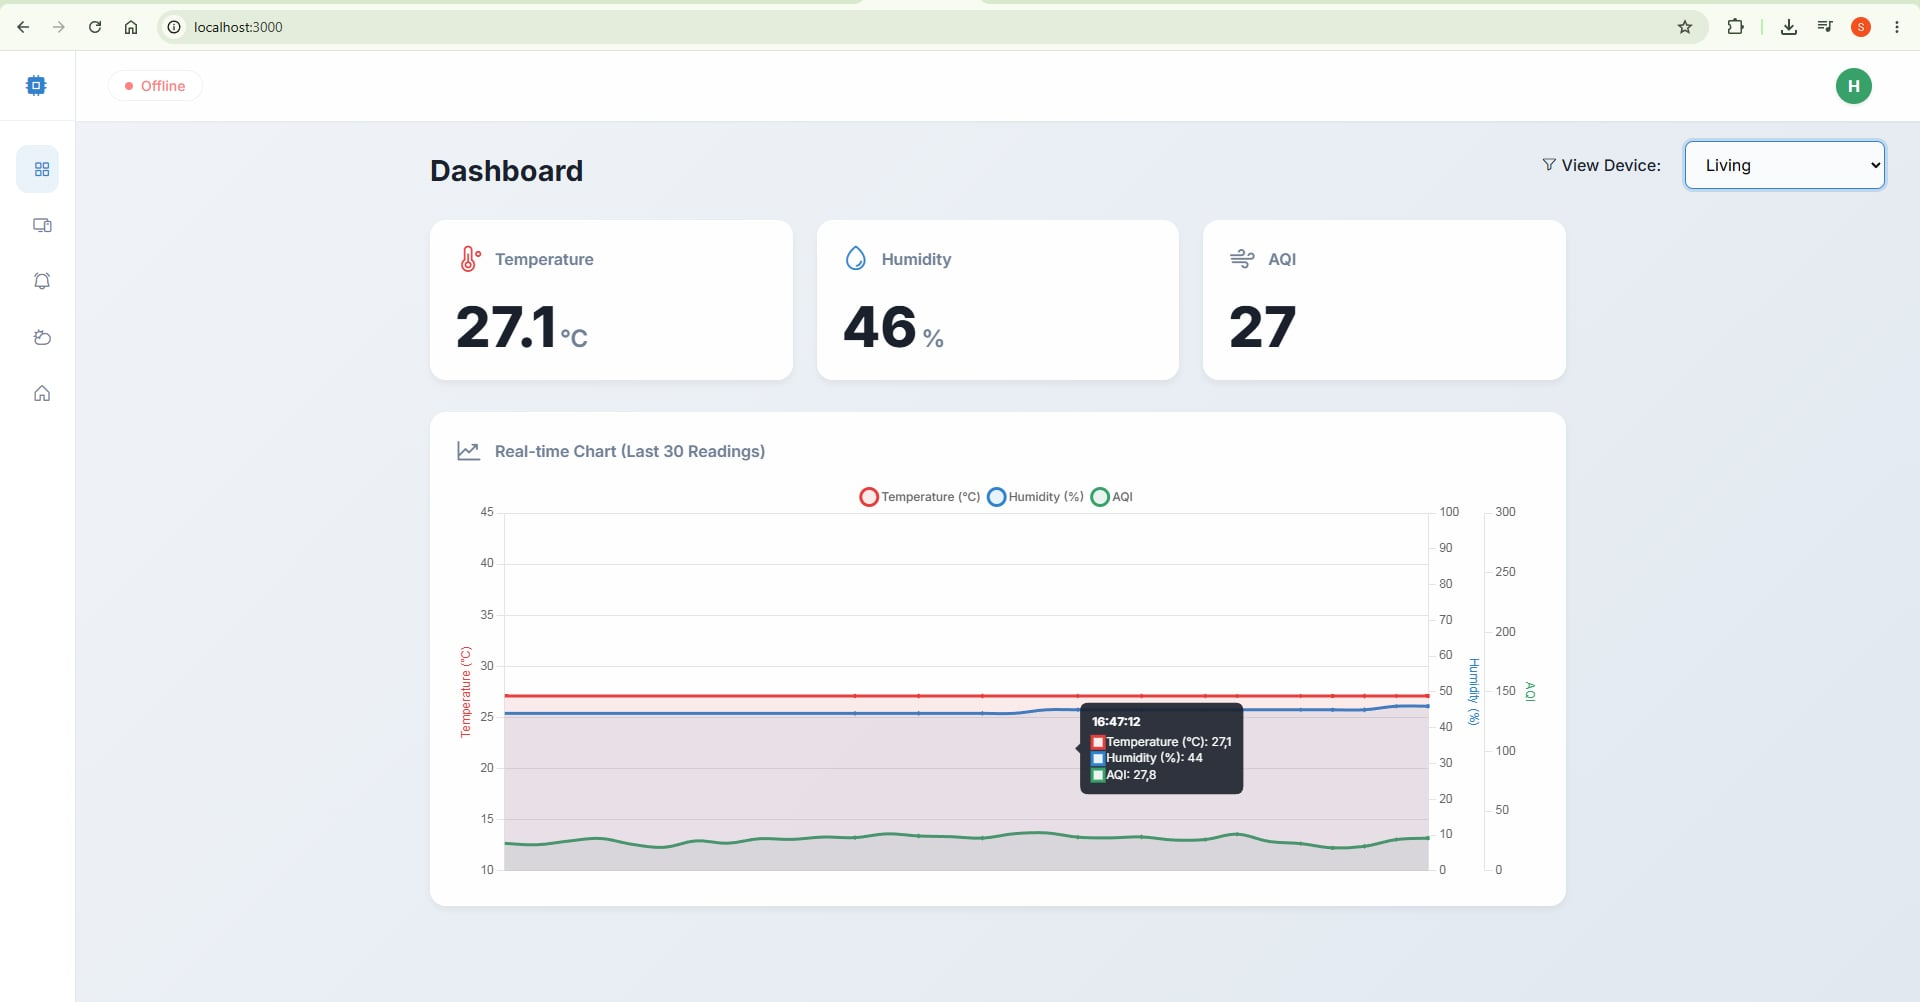
\includegraphics[width=\textwidth]{ui_dashboard}
  \caption{Giao diện Dashboard chính hiển thị dữ liệu realtime}
  \label{fig:ui_dashboard}
\end{figure}

\begin{figure}[H]
  \centering
  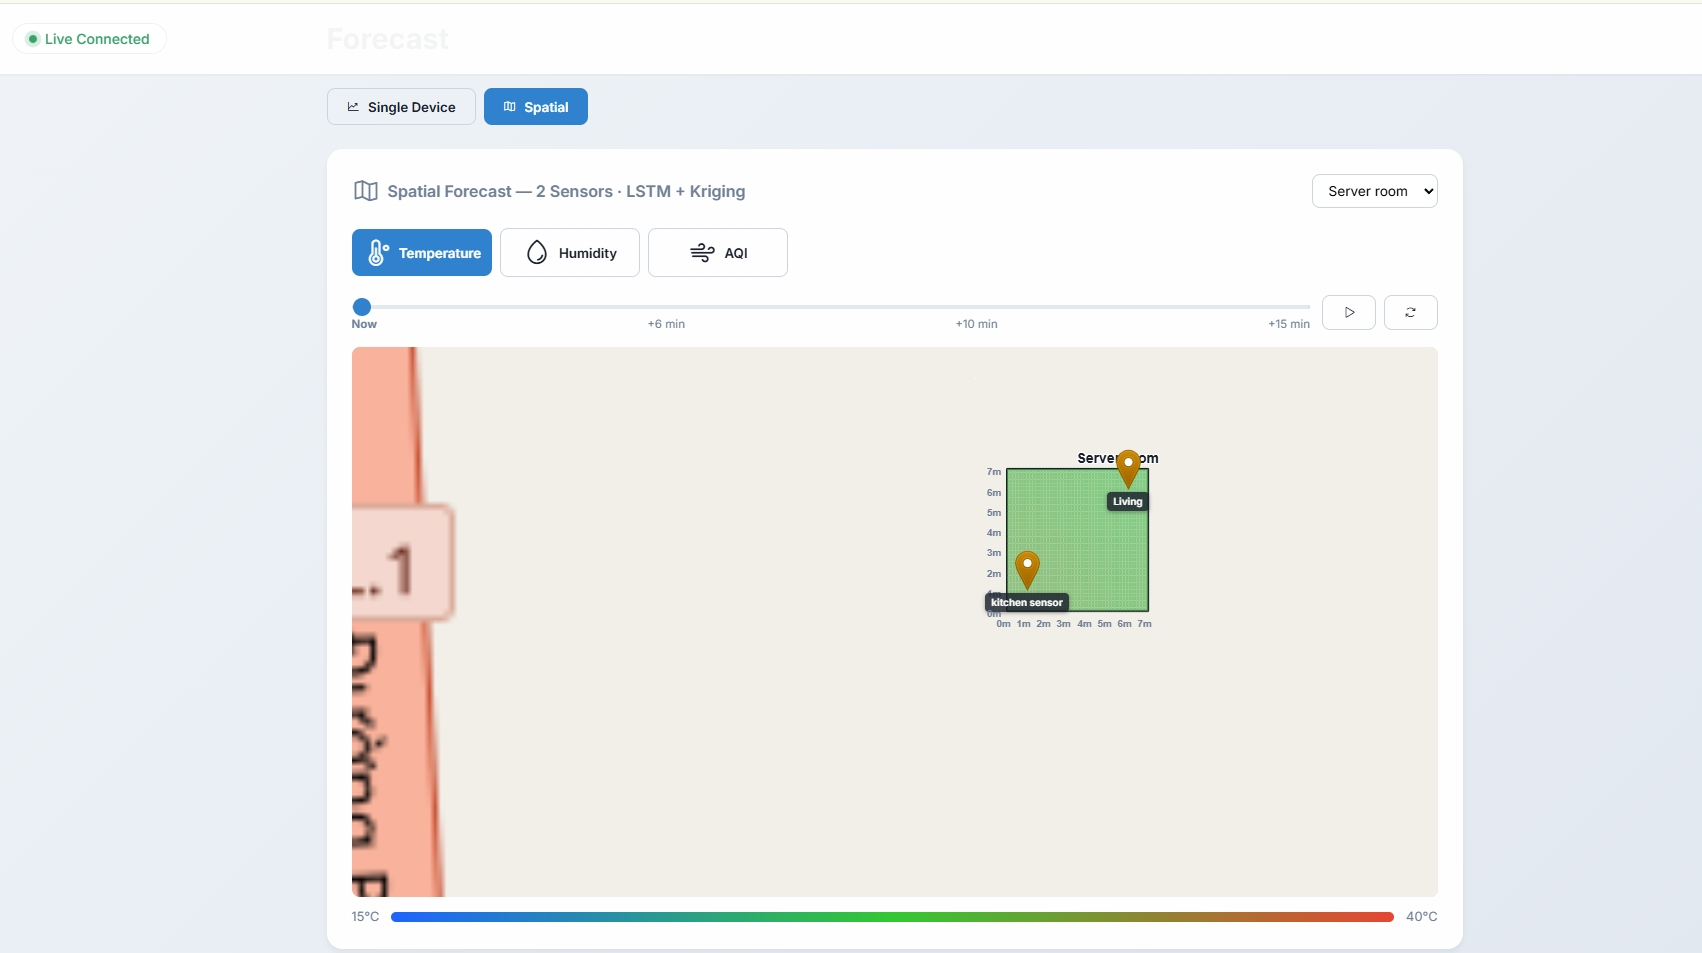
\includegraphics[width=\textwidth]{system_spatial_forecast}
  \caption{Giao diện chức năng dự báo không gian (Spatial Forecast)}
  \label{fig:ui_heatmap}
\end{figure}

%------------------------------------------------------------
\section{Xây dựng hệ thống}
\label{sec:design:impl}
%------------------------------------------------------------

\subsection{Thư viện và công cụ sử dụng}
\label{subsec:design:tools}

\begin{table}[H]
  \centering
  \caption{Danh sách thư viện và công cụ sử dụng}
  \label{tab:tools}
  \begin{tabularx}{\textwidth}{p{2.5cm} p{3.5cm} p{2cm} X}
    \toprule
    \textbf{Mục đích} & \textbf{Thư viện/Công cụ}
      & \textbf{Phiên bản} & \textbf{Ghi chú} \\
    \midrule
    Firmware IDE  & Arduino IDE     & 2.x     & Biên dịch C++ ESP32 \\
    MQTT Client   & PubSubClient    & 2.8     & MQTT trên ESP32 \\
    JSON (FW)     & ArduinoJson     & 6.x     & Đóng gói payload \\
    Cảm biến      & DHT sensor lib  & 1.4     & Đọc DHT11 \\
    Backend FW    & Node.js         & 18 LTS  & Runtime JavaScript \\
    Web framework & Express         & 4.x     & REST API \\
    MQTT Broker   & Aedes           & 0.50    & Broker tích hợp \\
    Realtime      & Socket.io       & 4.x     & WebSocket server \\
    Database      & PostgreSQL      & 15      & RDBMS chính \\
    ORM/Query     & node-postgres   & 8.x     & PostgreSQL client \\
    Auth          & jsonwebtoken    & 9.x     & JWT \\
    Password      & bcrypt          & 5.x     & Hash mật khẩu \\
    Email         & nodemailer      & 6.x     & Gửi cảnh báo \\
    ML Framework  & PyTorch         & 2.x     & Huấn luyện LSTM \\
    ML API        & FastAPI         & 0.110   & Serve ML inference \\
    Nội suy       & pykrige         & 1.7     & Kriging \\
    Nội suy       & scipy           & 1.12    & IDW \\
    Scaler        & scikit-learn    & 1.4     & MinMaxScaler \\
    Frontend      & React           & 19      & UI framework \\
    Build tool    & Vite            & 5.x     & Bundler \\
    Biểu đồ       & Chart.js        & 4.x     & Vẽ biểu đồ \\
    Bản đồ        & Leaflet         & 1.9     & Render heatmap \\
    Quản lý mã    & Git / GitHub    & ---     & Version control \\
    \bottomrule
  \end{tabularx}
\end{table}

\subsection{Kết quả đạt được}
\label{subsec:design:result}

Sau quá trình thiết kế và triển khai, đồ án đã xây dựng thành công hệ
thống hoàn chỉnh với đầy đủ các thành phần hoạt động ổn định. Kết quả
cụ thể từng thành phần:

\begin{itemize}[leftmargin=2cm]
  \item \textbf{Node cảm biến ESP32:} Hoạt động ổn định, đọc và gửi
    dữ liệu định kỳ 5 giây qua MQTT. Cơ chế tự động reconnect đảm bảo
    node phục hồi kết nối sau khi mất mạng mà không cần can thiệp thủ
    công.
  \item \textbf{Backend Node.js:} Tiếp nhận và xử lý dữ liệu từ nhiều
    node đồng thời. MQTT broker Aedes và Socket.io hoạt động ổn định
    trong cùng tiến trình. API trả về kết quả trong thời gian trung
    bình dưới 100ms cho các truy vấn dữ liệu thông thường.
  \item \textbf{FastAPI ML service:} Inference LSTM hoàn thành trong
    dưới 200ms cho một node (window 30, horizon 15). Kriging tính toán
    lưới 40$\times$50 trong khoảng 1--2 giây tùy số lượng node.
  \item \textbf{Dashboard React:} Biểu đồ Chart.js cập nhật realtime
    khi nhận event Socket.io, không cần tải lại trang. Heatmap Leaflet
    render đúng và trực quan trên các trình duyệt hiện đại.
  \item \textbf{Mô hình LSTM:} Huấn luyện hội tụ tốt trên tập dữ liệu
    thu thập được. Loss curve thể hiện xu hướng giảm đều và ổn định
    giữa training loss và validation loss.
\end{itemize}

Một số ảnh tiêu biểu được chọn để chèn trực tiếp trong nội dung báo cáo, minh họa toàn bộ các giao diện chức năng của hệ thống[cite: 122, 136].

% CỤM 1: Xác thực & Quản lý thiết bị (STT 1 - 4)
\begin{figure}[H]
  \centering
  \begin{subfigure}{0.48\textwidth}
    \centering
    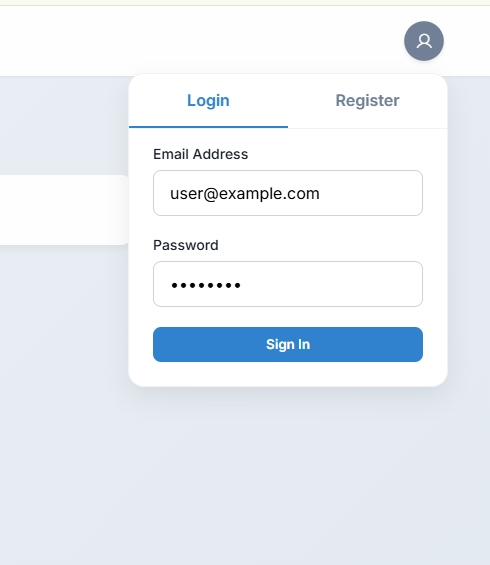
\includegraphics[width=\textwidth]{system_login.jpg}
    \caption{Màn hình đăng nhập}
  \end{subfigure}
  \hfill
  \begin{subfigure}{0.48\textwidth}
    \centering
    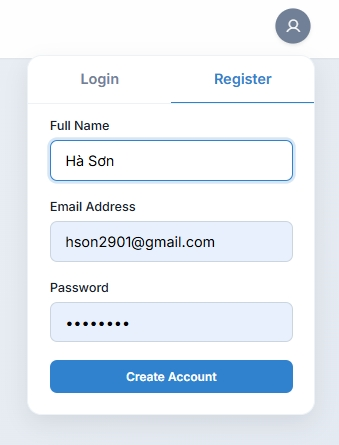
\includegraphics[width=\textwidth]{system_register.jpg}
    \caption{Màn hình đăng ký}
  \end{subfigure}

  \vspace{0.4cm}
  \begin{subfigure}{0.48\textwidth}
    \centering
    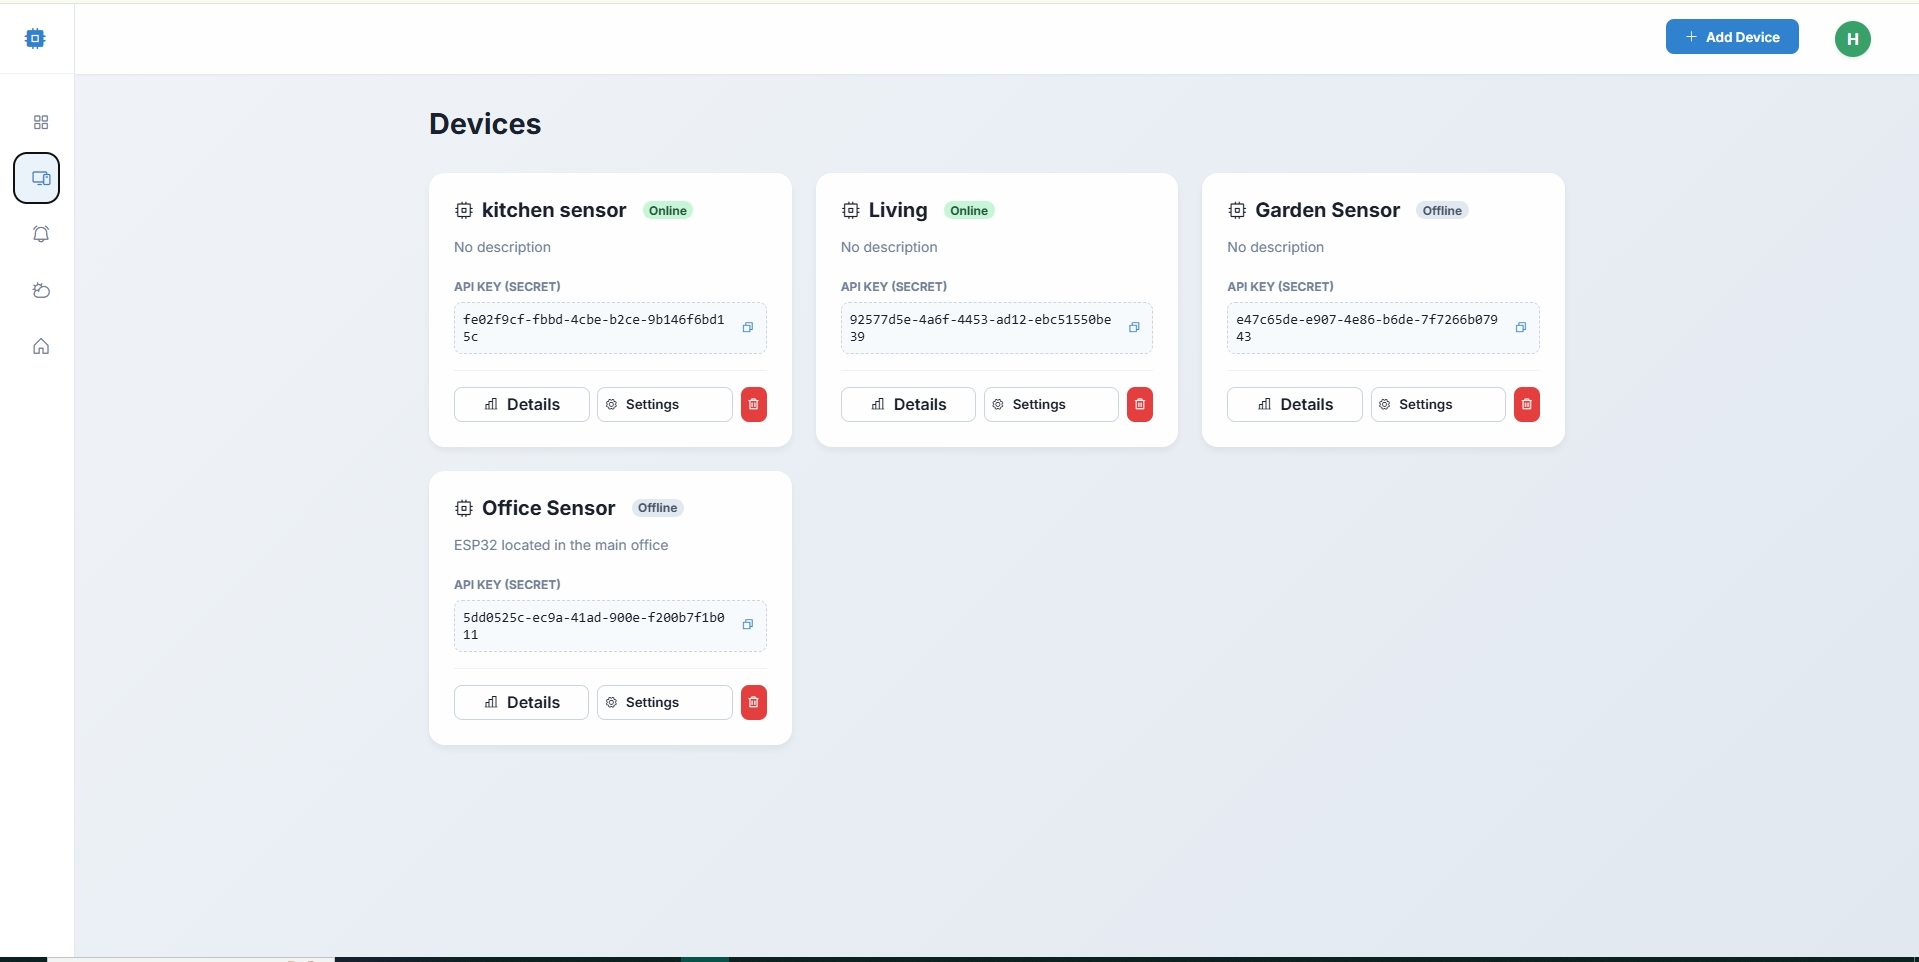
\includegraphics[width=\textwidth]{system_devices.jpg}
    \caption{Danh sách thiết bị IoT}
  \end{subfigure}
  \hfill
  \begin{subfigure}{0.48\textwidth}
    \centering
    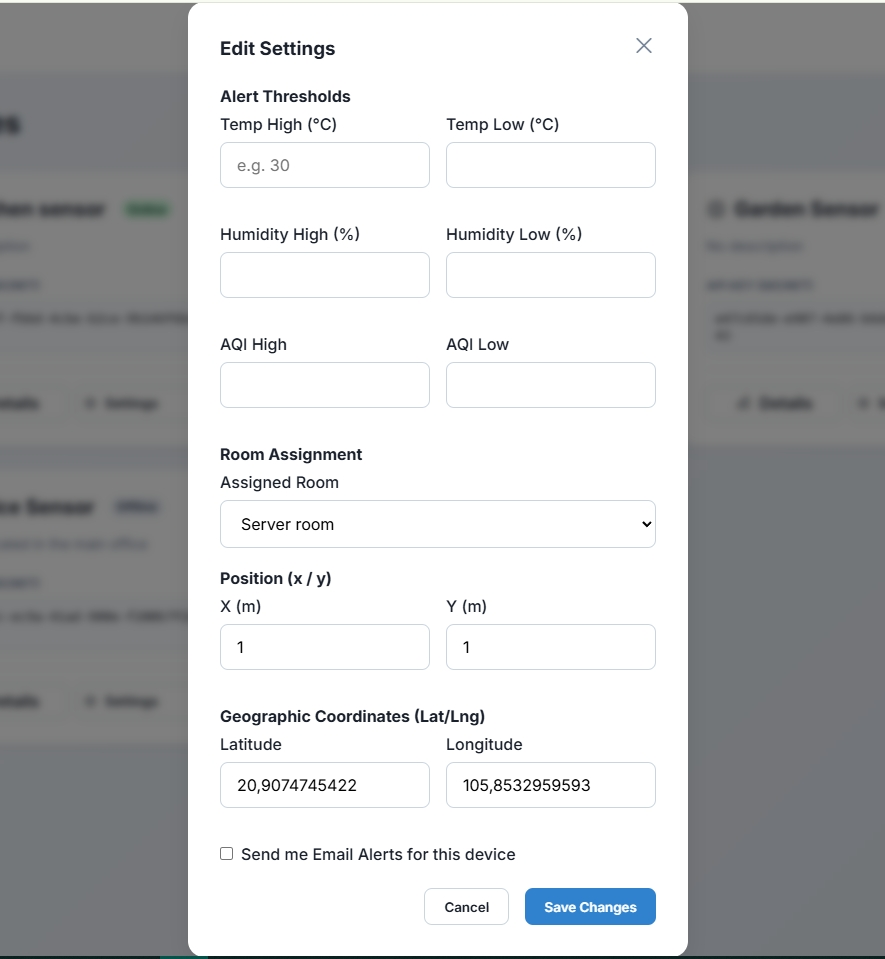
\includegraphics[width=\textwidth]{system_devices_setting.jpg}
    \caption{Cấu hình ngưỡng cảnh báo}
  \end{subfigure}
  \caption{Giao diện chức năng hệ thống --- Đăng nhập, đăng ký và quản lý thiết bị}
  \label{fig:system_demo_part1}
\end{figure}

% CỤM 2: Dashboard & Chi tiết thiết bị (STT 5 - 8)
\begin{figure}[H]
  \centering
  \begin{subfigure}{0.48\textwidth}
    \centering
    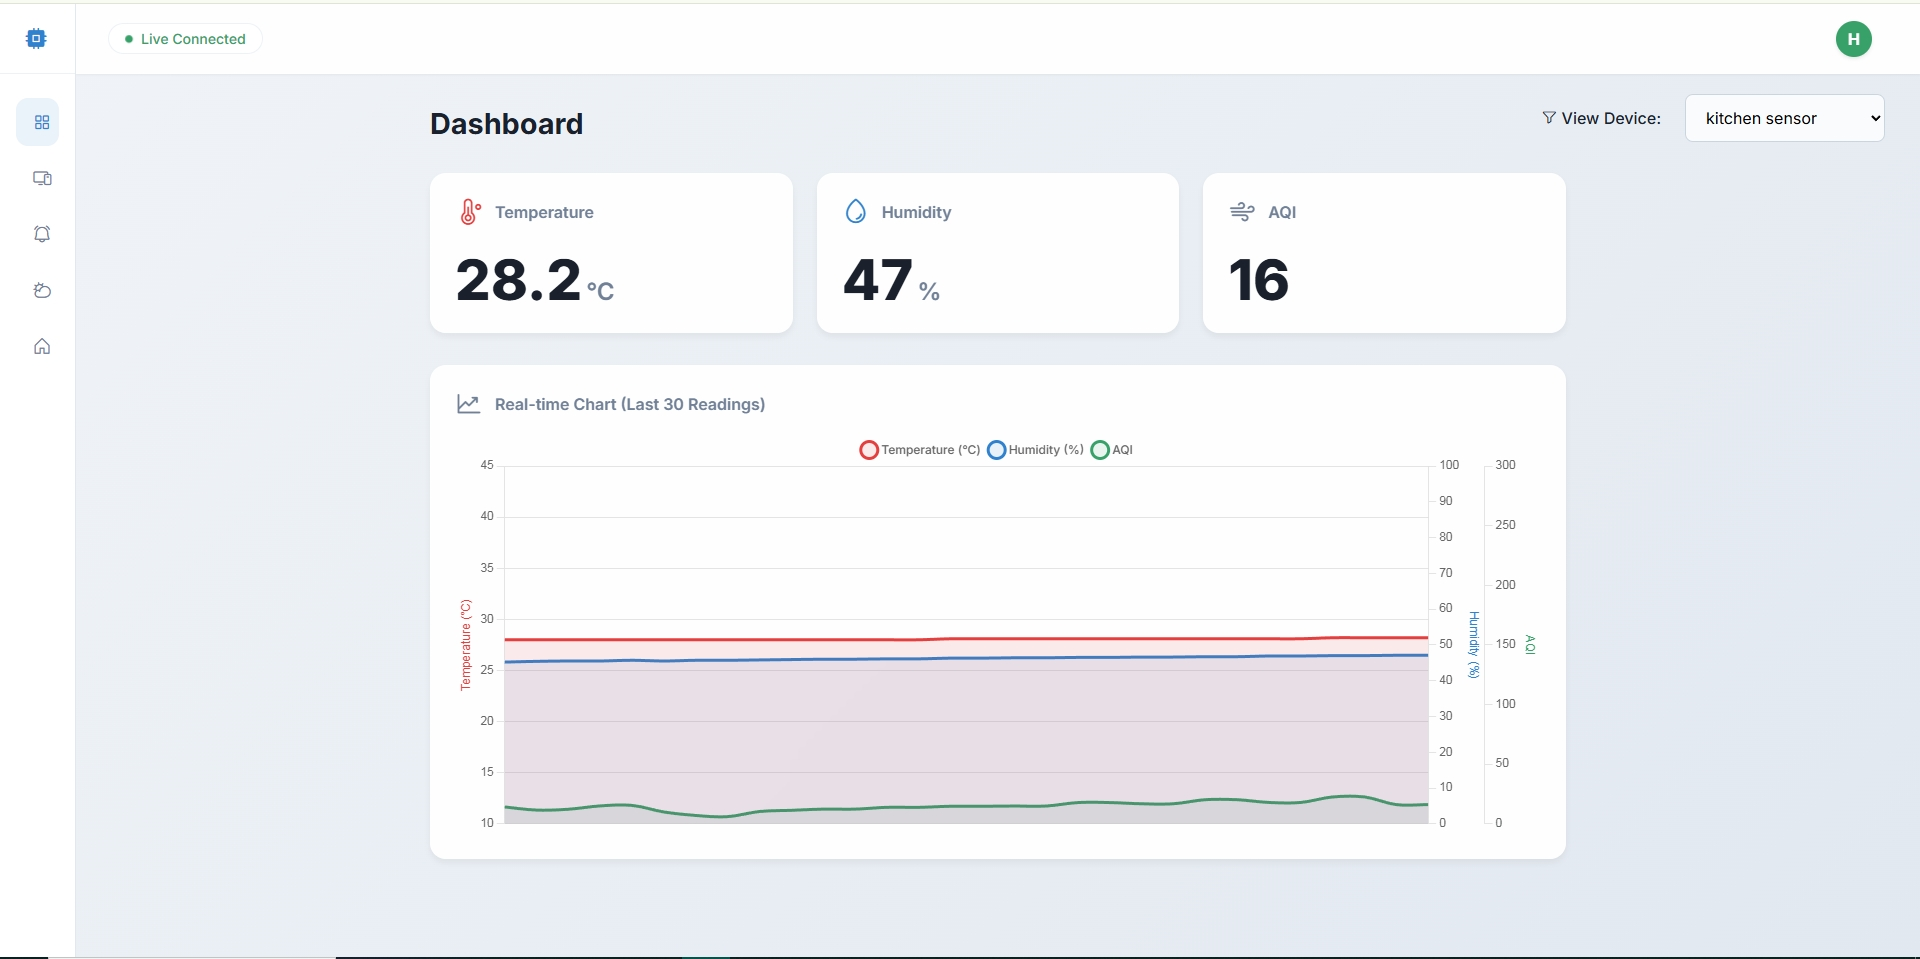
\includegraphics[width=\textwidth]{system_dashboard.jpg}
    \caption{Dashboard tổng quan}
  \end{subfigure}
  \hfill
  \begin{subfigure}{0.48\textwidth}
    \centering
    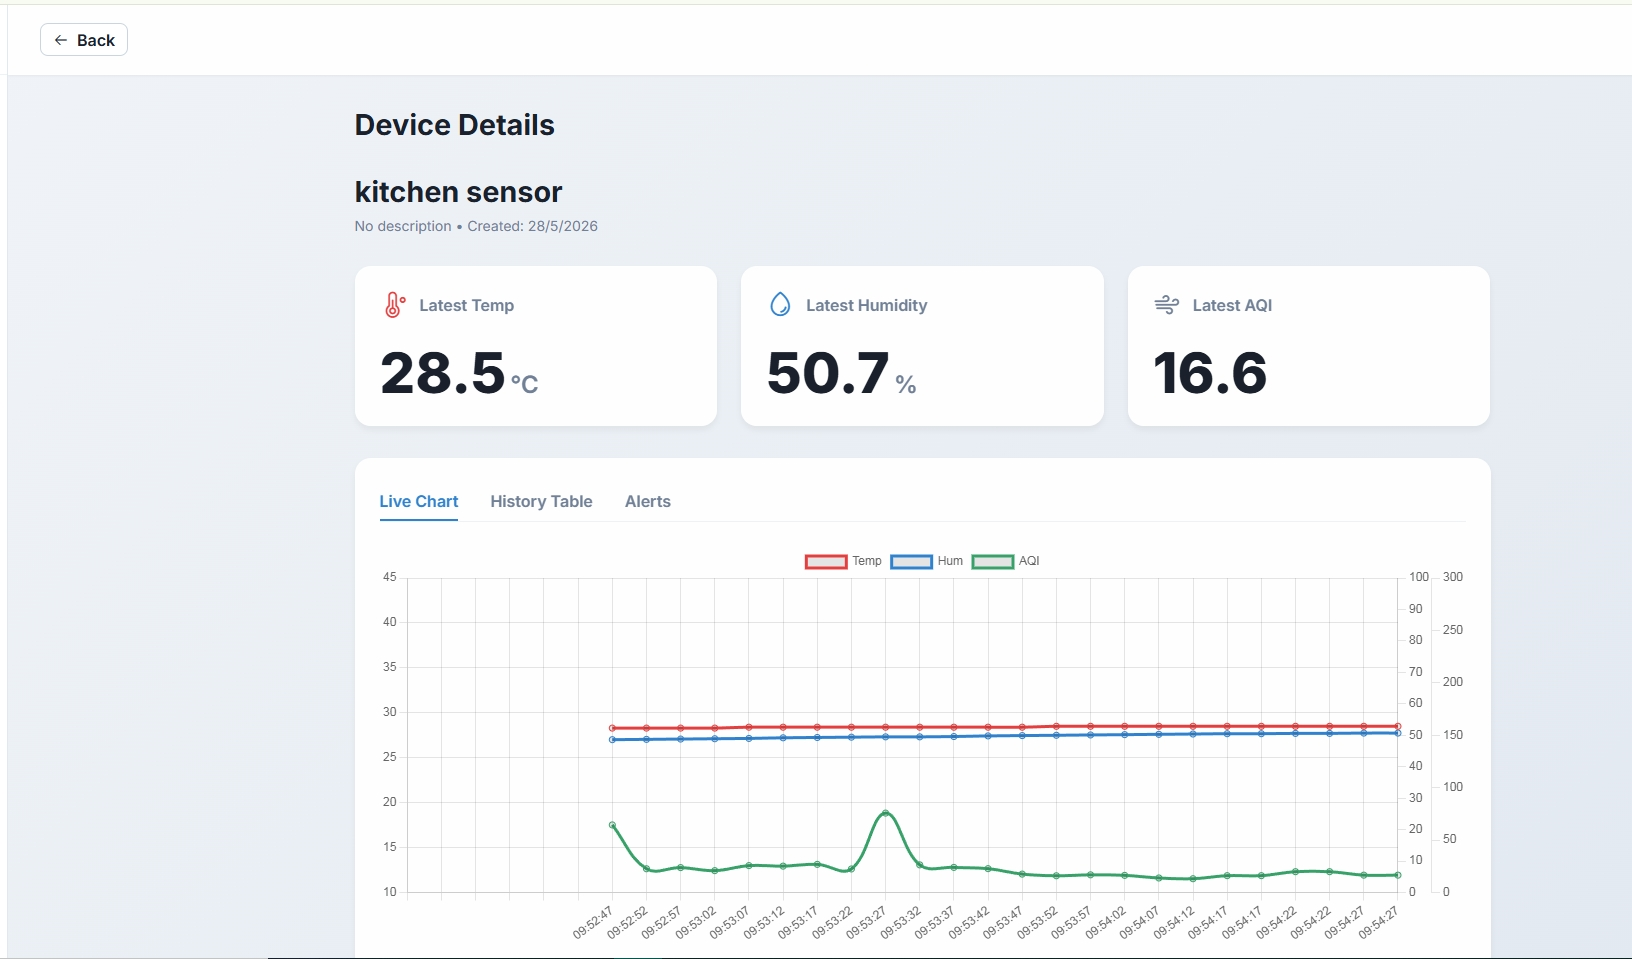
\includegraphics[width=\textwidth]{system_devices_detail_chart.jpg}
    \caption{Biểu đồ chi tiết thiết bị (Live Chart)}
  \end{subfigure}

  \vspace{0.4cm}
  \begin{subfigure}{0.48\textwidth}
    \centering
    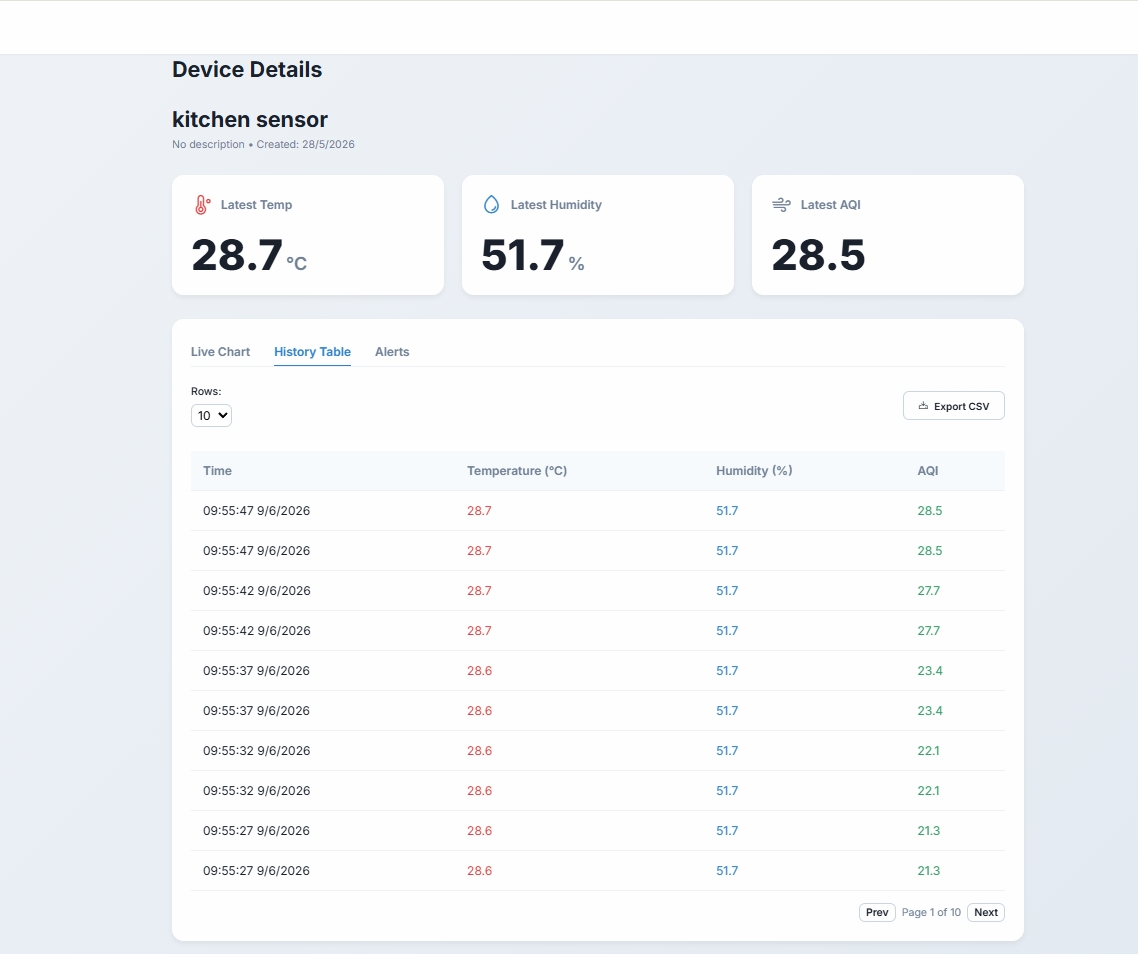
\includegraphics[width=\textwidth]{system_devices_detail_history.jpg}
    \caption{Lịch sử dữ liệu cảm biến}
  \end{subfigure}
  \hfill
  \begin{subfigure}{0.48\textwidth}
    \centering
    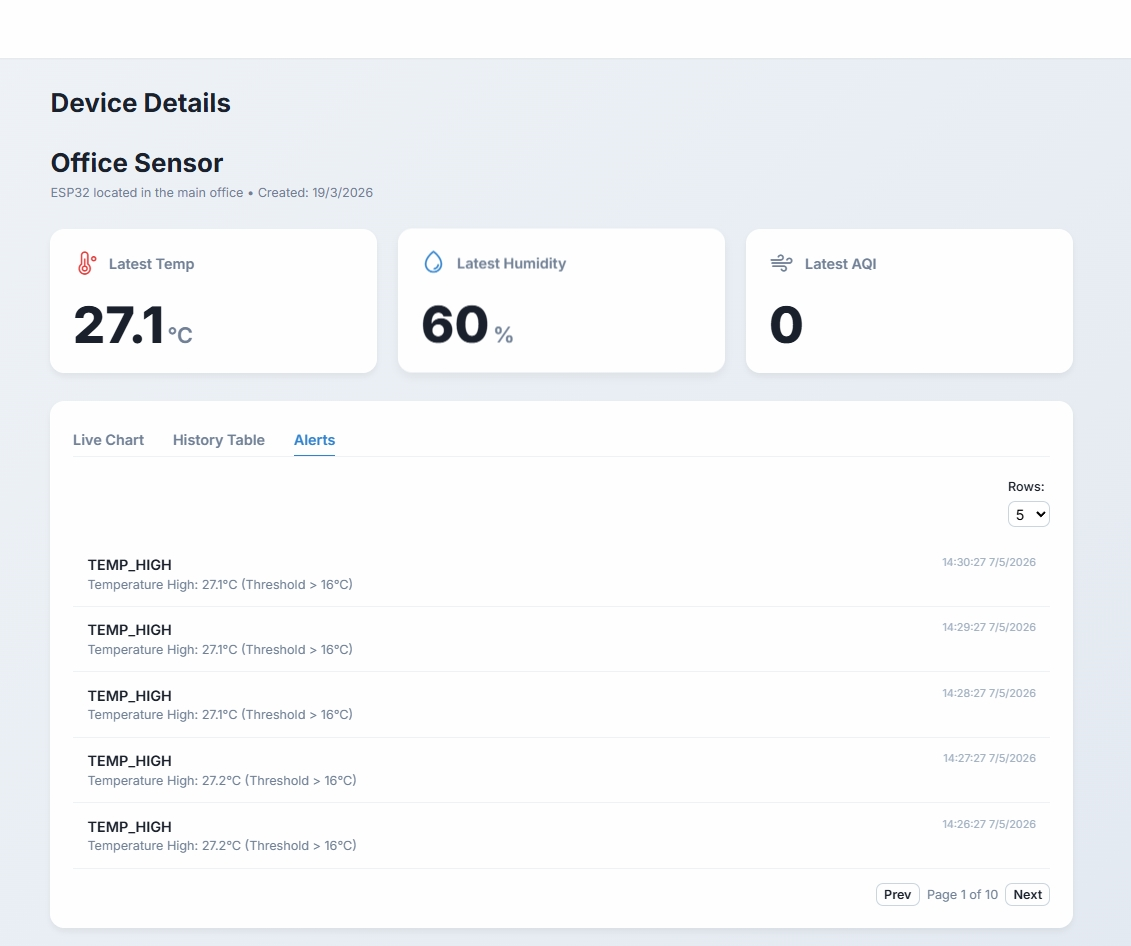
\includegraphics[width=\textwidth]{system_devices_detail_alert.jpg}
    \caption{Lịch sử cảnh báo của thiết bị}
  \end{subfigure}
  \caption{Giao diện chức năng hệ thống --- Dashboard và các tab chi tiết thiết bị}
  \label{fig:system_demo_part2}
\end{figure}

% CỤM 3: Dự báo & Quản lý không gian, Cảnh báo hệ thống (STT 9 - 13)
\begin{figure}[H]
  \centering
  \begin{subfigure}{0.48\textwidth}
    \centering
    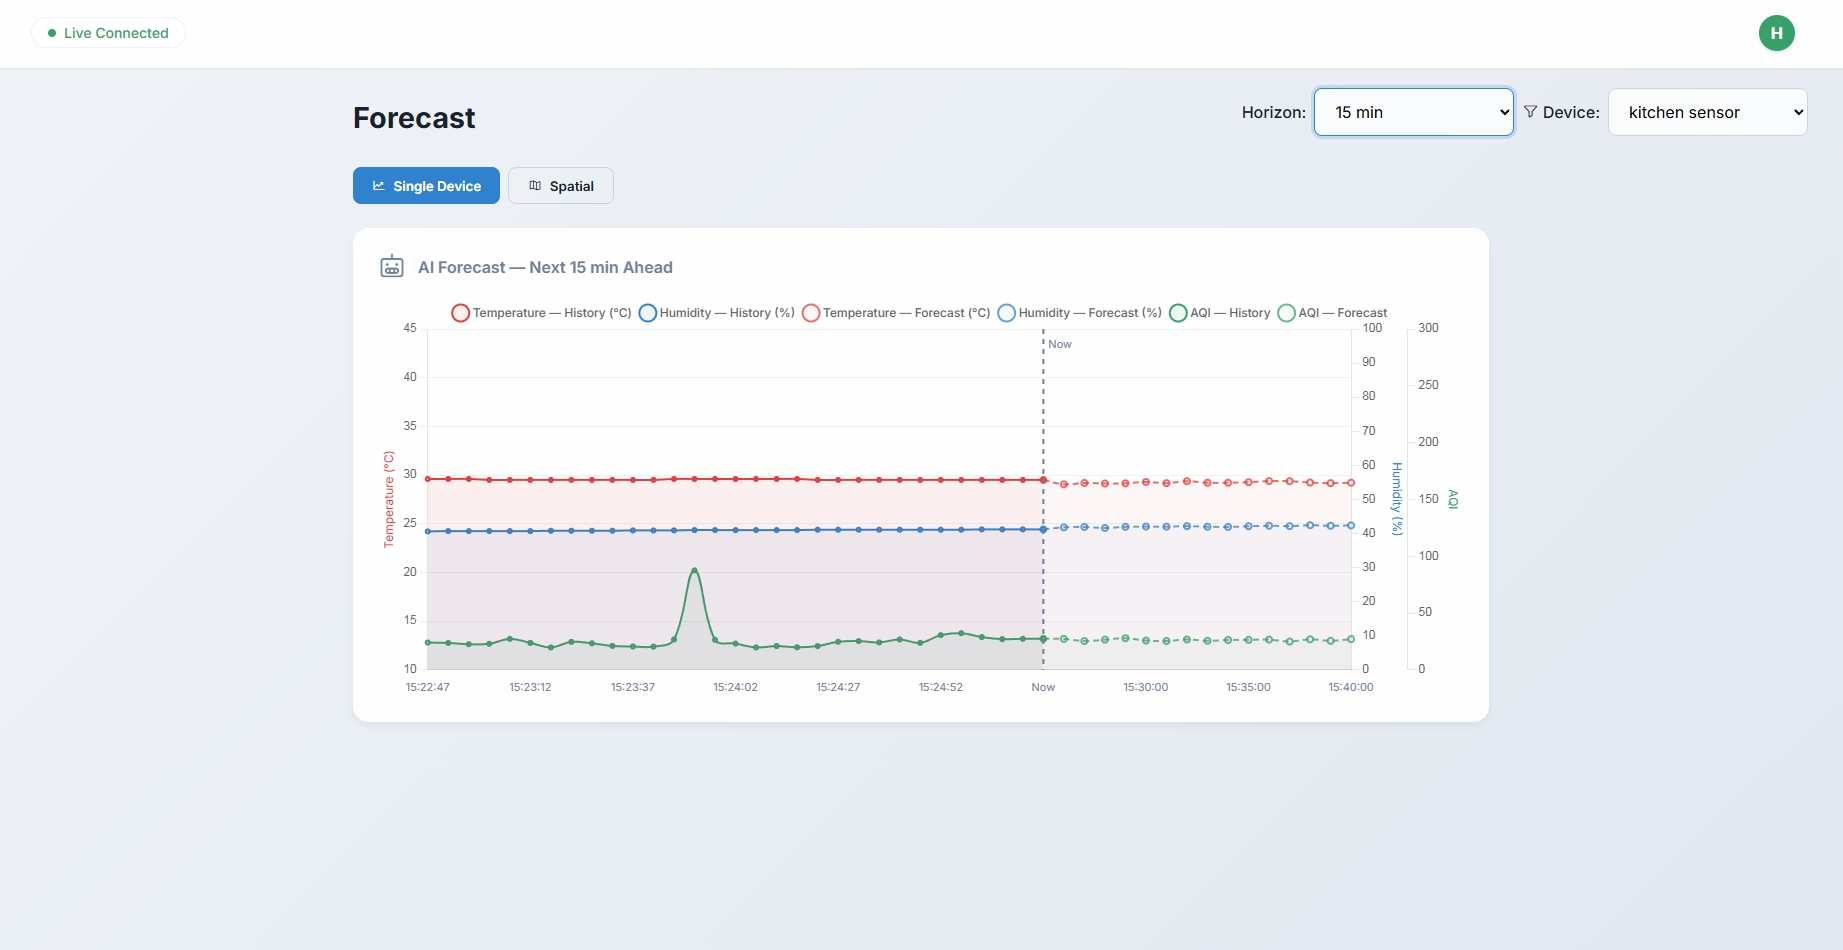
\includegraphics[width=\textwidth]{system_forecast.jpg}
    \caption{Dự báo chuỗi thời gian LSTM}
  \end{subfigure}
  \hfill
  \begin{subfigure}{0.48\textwidth}
    \centering
    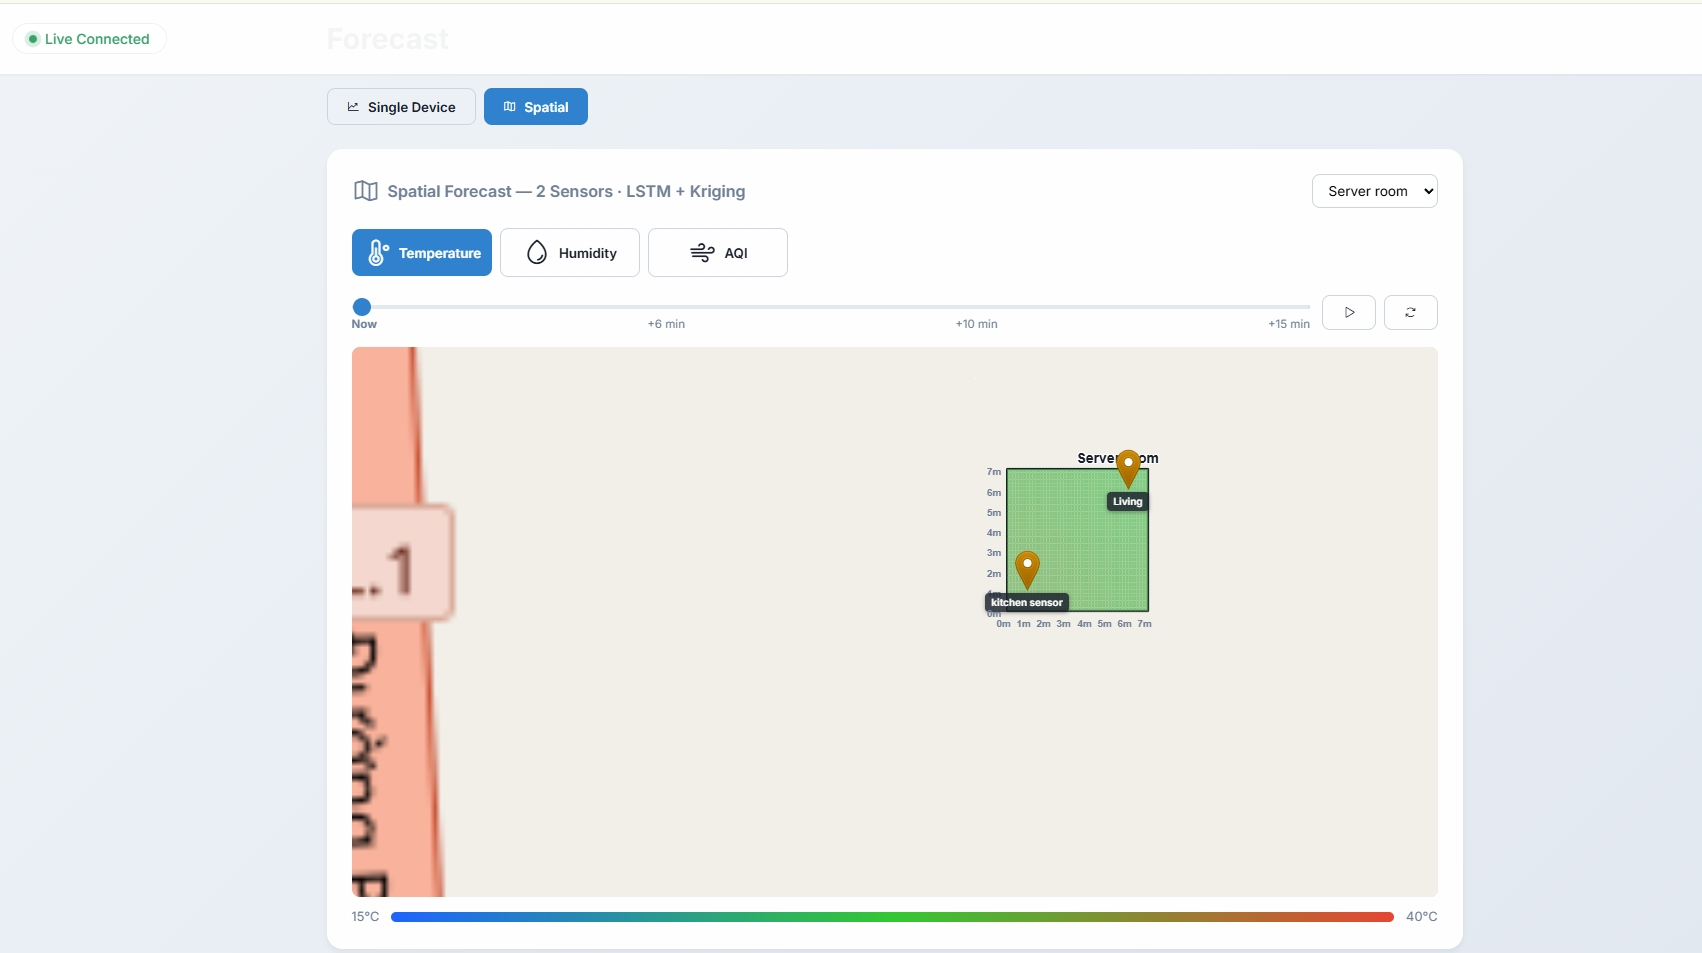
\includegraphics[width=\textwidth]{system_spatial_forecast.jpg}
    \caption{Heatmap không gian}
  \end{subfigure}

  \vspace{0.4cm}
  \begin{subfigure}{0.48\textwidth}
    \centering
    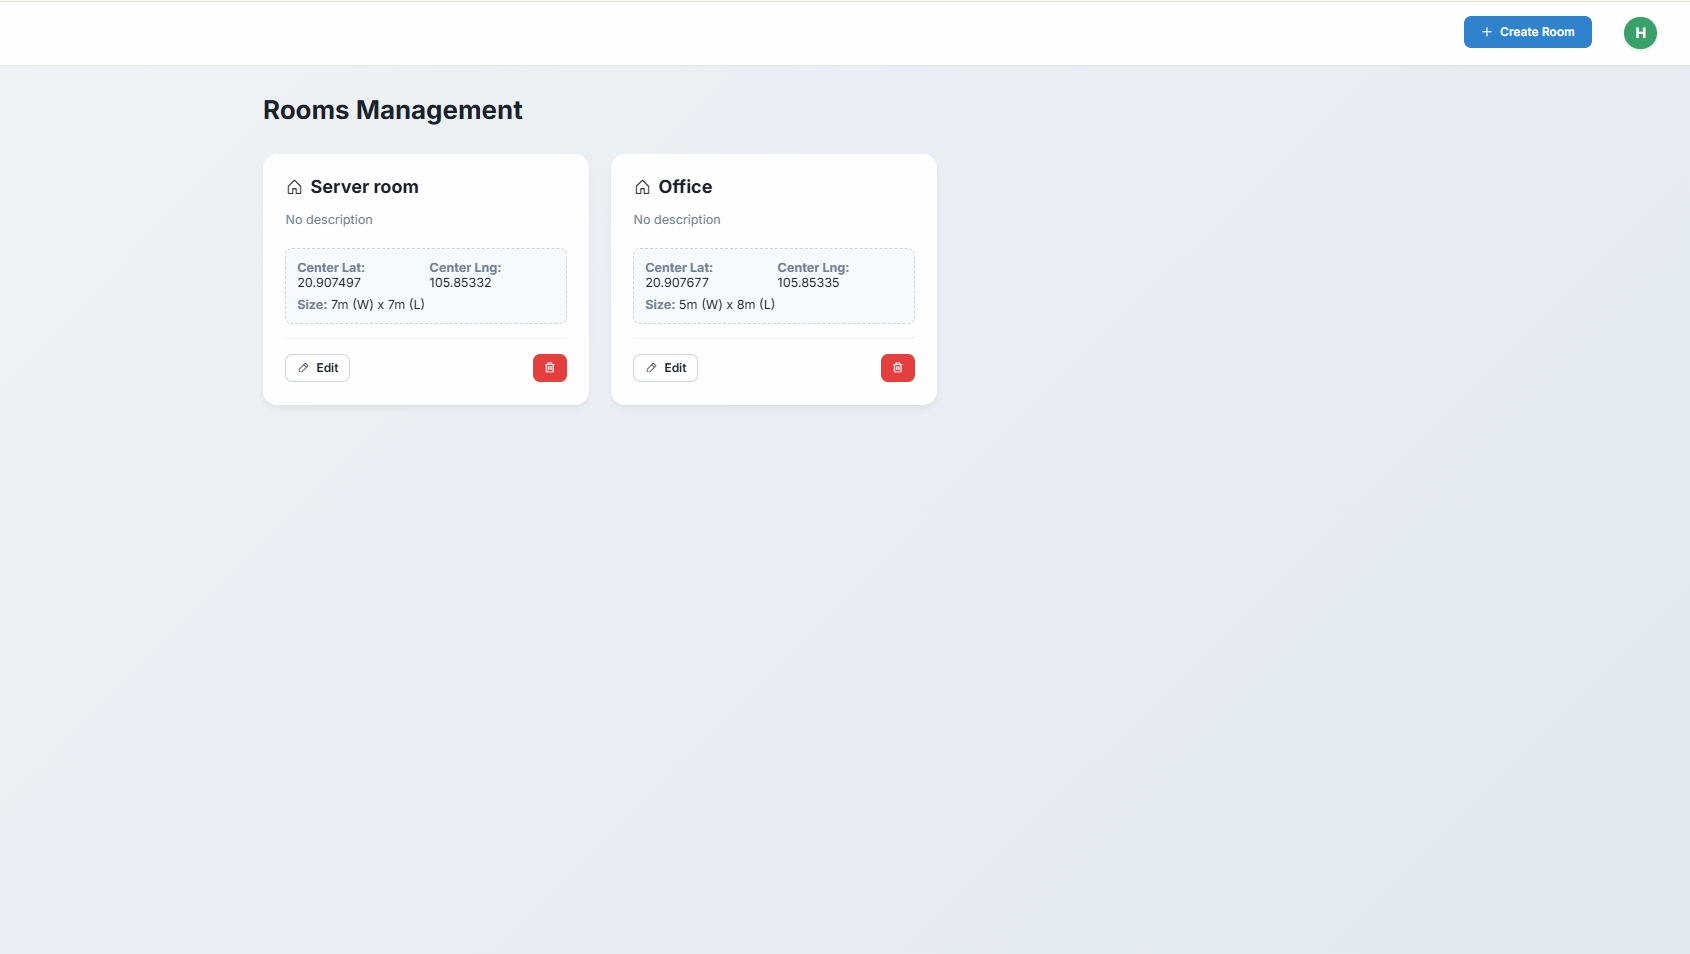
\includegraphics[width=\textwidth]{system_rooms.jpg}
    \caption{Quản lý danh sách phòng}
  \end{subfigure}
  \hfill
  \begin{subfigure}{0.48\textwidth}
    \centering
    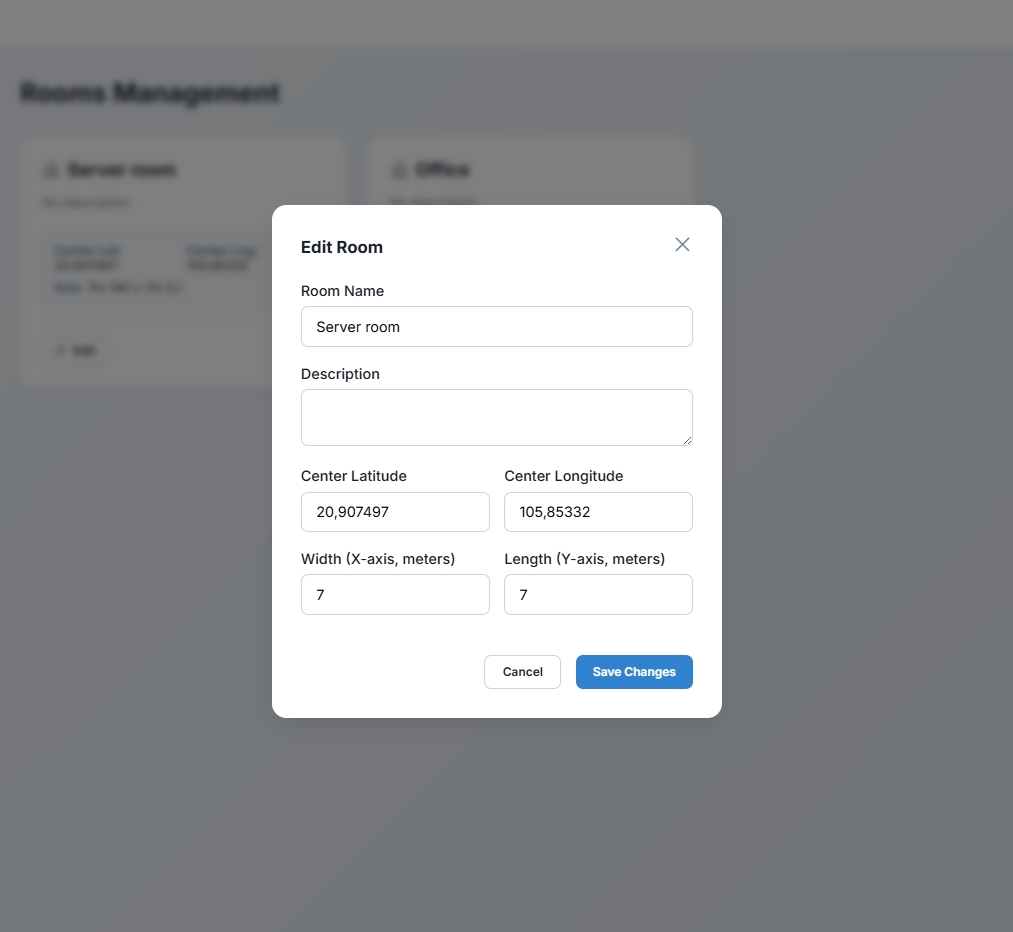
\includegraphics[width=\textwidth]{system_rooms_config.jpg}
    \caption{Cấu hình kích thước và vị trí node}
  \end{subfigure}

  \vspace{0.4cm}
  \begin{subfigure}{0.48\textwidth}
    \centering
    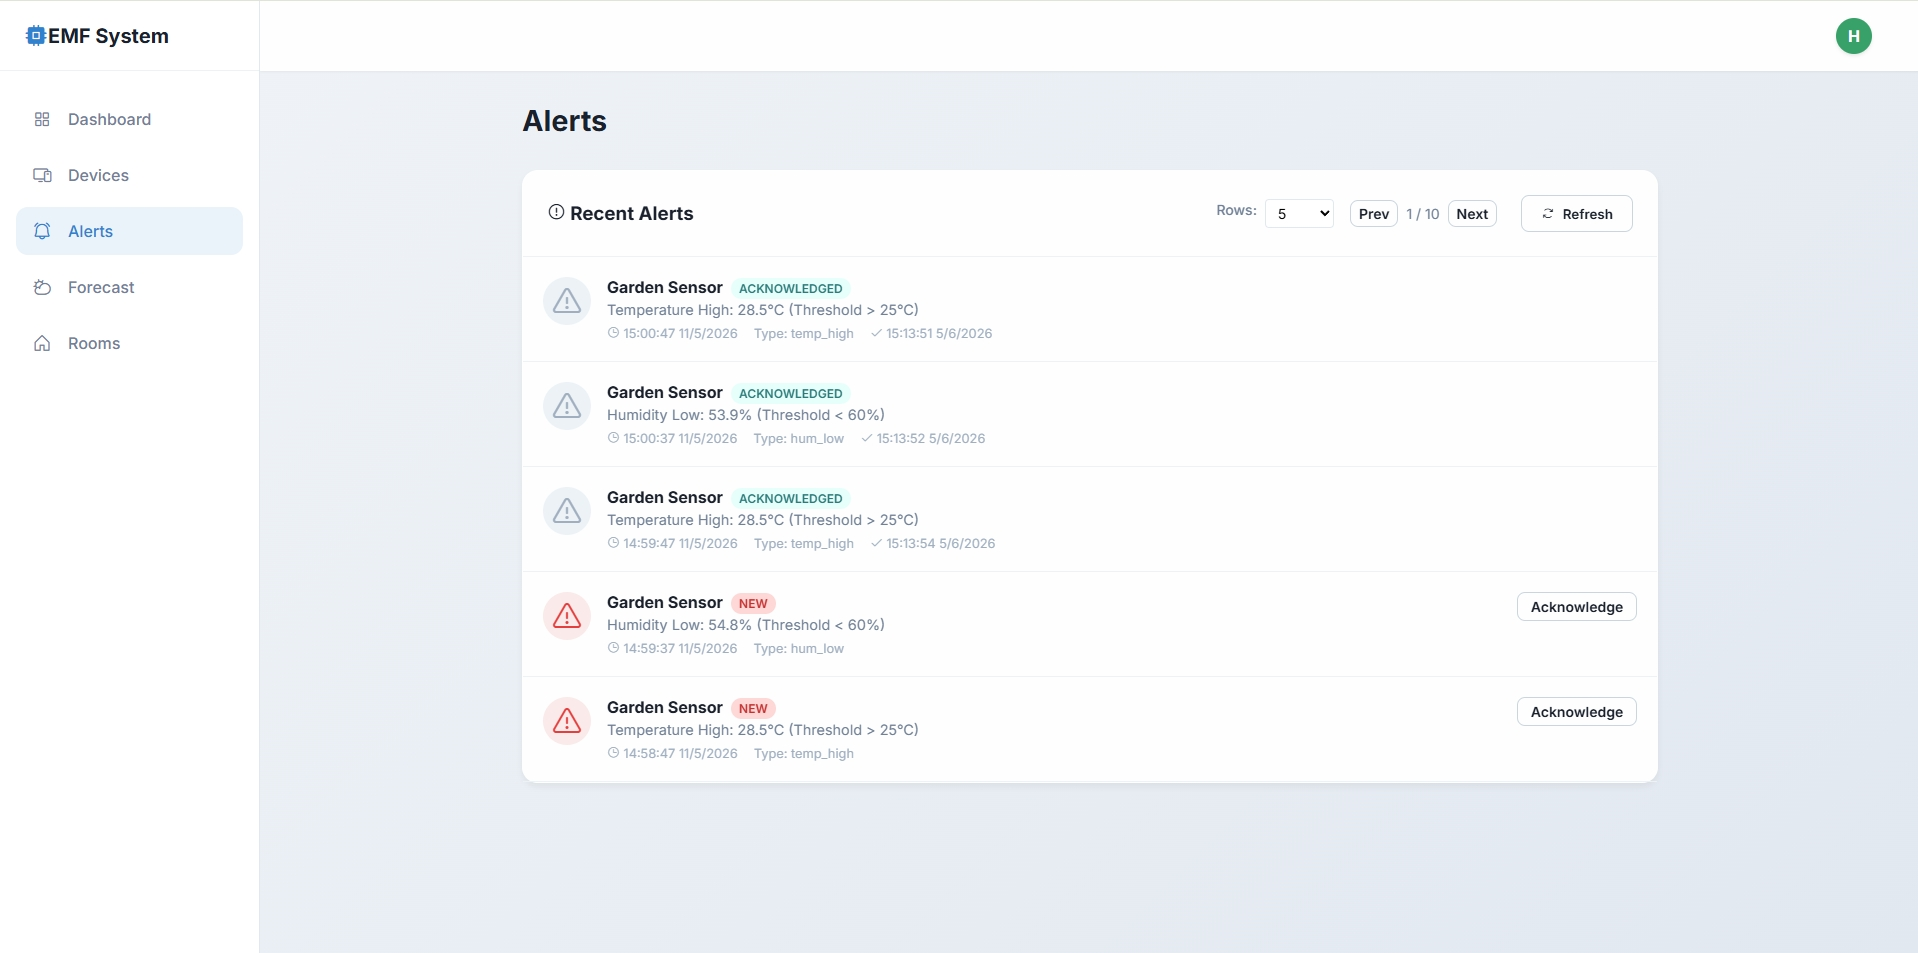
\includegraphics[width=\textwidth]{system_alerts.jpg}
    \caption{Danh sách cảnh báo hệ thống}
  \end{subfigure}
  \caption{Giao diện dự báo thời gian/không gian, quản lý phòng và cảnh báo hệ thống}
  \label{fig:system_demo_part3}
\end{figure}

\subsection{Minh họa các chức năng chính}
\label{subsec:design:demo}

\textbf{Chức năng 1 --- Đăng ký node IoT tự động:} Khi node ESP32
khởi động lần đầu, hệ thống tự động cấp phát \texttt{api\_key} qua
MQTT mà không cần thao tác thủ công từ phía người dùng. Node sẵn sàng
gửi dữ liệu trong vòng vài giây sau khi kết nối Wi-Fi thành công.

\textbf{Chức năng 2 --- Giám sát realtime:} Biểu đồ nhiệt độ và độ
ẩm trên dashboard cập nhật tức thì mỗi khi node gửi dữ liệu mới qua
Socket.io, không cần tải lại trang. Người dùng có thể theo dõi nhiều
node cùng lúc trên cùng giao diện.

\textbf{Chức năng 3 --- Dự báo chuỗi thời gian:} Người dùng chọn node
và khoảng thời gian, hệ thống trả về biểu đồ dự báo 15 bước tiếp theo
(màu khác để phân biệt với dữ liệu lịch sử). Thời gian phản hồi từ
khi nhấn nút đến khi hiện kết quả dưới 3 giây.

\textbf{Chức năng 4 --- Heatmap phân bố không gian:} Từ dữ liệu của
các node trong phòng, hệ thống render heatmap nhiệt độ/độ ẩm phủ lên
bản đồ sàn phòng. Gradient màu từ xanh lam (mát/khô) đến đỏ
(nóng/ẩm) giúp người dùng nhận biết vùng bất thường trực quan.

\textbf{Chức năng 5 --- Cảnh báo tự động:} Khi nhiệt độ hoặc độ ẩm
vượt ngưỡng cài đặt, hệ thống tự động ghi alert, hiển thị thông báo
trên dashboard và gửi email đến người dùng trong vòng 30 giây.

%------------------------------------------------------------
\section{Kiểm thử}
\label{sec:design:test}
%------------------------------------------------------------

Kiểm thử được thực hiện theo phương pháp hộp đen (black-box), tập
trung vào đầu vào và đầu ra quan sát được mà không xét cấu trúc nội
bộ mã nguồn.

\begin{table}[H]
  \centering
  \caption{Kiểm thử chức năng đăng ký và kết nối node IoT}
  \label{tab:test_register}
  \begin{tabularx}{\textwidth}{p{4cm} X p{1.5cm}}
    \toprule
    \textbf{Trường hợp kiểm thử} & \textbf{Kết quả mong đợi}
      & \textbf{Kết quả} \\
    \midrule
    Node mới kết nối lần đầu
      & Backend tạo bản ghi device, sinh \texttt{api\_key}, gửi config
        về node qua MQTT
      & Đạt \\
    Node đã tồn tại kết nối lại
      & Backend trả về cấu hình hiện có, không tạo bản ghi mới
      & Đạt \\
    Wi-Fi mất kết nối giữa chừng
      & Node tự động reconnect sau 5 giây
      & Đạt \\
    \texttt{api\_key} không hợp lệ
      & Backend bỏ qua message, ghi log cảnh báo
      & Đạt \\
    \bottomrule
  \end{tabularx}
\end{table}

\begin{table}[H]
  \centering
  \caption{Kiểm thử chức năng thu thập và hiển thị dữ liệu realtime}
  \label{tab:test_realtime}
  \begin{tabularx}{\textwidth}{p{4cm} X p{1.5cm}}
    \toprule
    \textbf{Trường hợp kiểm thử} & \textbf{Kết quả mong đợi}
      & \textbf{Kết quả} \\
    \midrule
    Node gửi dữ liệu bình thường
      & Dashboard cập nhật biểu đồ trong dưới 2 giây
      & Đạt \\
    DHT11 trả về NaN (lỗi đọc)
      & Firmware bỏ qua chu kỳ đó, thử lại sau 5 giây
      & Đạt \\
    Nhiều node gửi đồng thời
      & Tất cả dữ liệu được lưu đúng, không bị mất
      & Đạt \\
    Client mở nhiều tab cùng lúc
      & Mỗi tab nhận đúng dữ liệu của node đang subscribe
      & Đạt \\
    \bottomrule
  \end{tabularx}
\end{table}

\begin{table}[H]
  \centering
  \caption{Kiểm thử chức năng dự báo và heatmap}
  \label{tab:test_forecast}
  \begin{tabularx}{\textwidth}{p{4cm} X p{1.5cm}}
    \toprule
    \textbf{Trường hợp kiểm thử} & \textbf{Kết quả mong đợi}
      & \textbf{Kết quả} \\
    \midrule
    Yêu cầu dự báo khi đủ 30 bản ghi
      & FastAPI trả về mảng 15 giá trị, dashboard hiển thị đúng
      & Đạt \\
    Yêu cầu dự báo khi chưa đủ 30 bản ghi
      & API trả về lỗi 400 kèm thông báo rõ ràng
      & Đạt \\
    FastAPI service bị dừng
      & Backend Node.js trả về lỗi 503, không crash
      & Đạt \\
    Heatmap với 1 node duy nhất
      & Hệ thống sinh node ảo bù biên, render được heatmap
      & Đạt \\
    \bottomrule
  \end{tabularx}
\end{table}

\begin{table}[H]
  \centering
  \caption{Kiểm thử chức năng cảnh báo}
  \label{tab:test_alert}
  \begin{tabularx}{\textwidth}{p{4cm} X p{1.5cm}}
    \toprule
    \textbf{Trường hợp kiểm thử} & \textbf{Kết quả mong đợi}
      & \textbf{Kết quả} \\
    \midrule
    Nhiệt độ vượt ngưỡng cao
      & Alert được tạo trong DB, email gửi đến người dùng
      & Đạt \\
    Độ ẩm dưới ngưỡng thấp
      & Alert được tạo, hiển thị trên dashboard
      & Đạt \\
    Xác nhận (acknowledge) alert
      & Alert được đánh dấu đã xử lý, không gửi email lần nữa
      & Đạt \\
    Tắt tính năng notify\_email
      & Alert vẫn ghi DB nhưng không gửi email
      & Đạt \\
    \bottomrule
  \end{tabularx}
\end{table}

%------------------------------------------------------------
\section{Triển khai}
\label{sec:design:deploy}
%------------------------------------------------------------

\subsection{Môi trường triển khai}
\label{subsec:design:deploy:env}

Hệ thống được triển khai và kiểm thử trong môi trường phòng lab với
cấu hình cụ thể như sau:

\begin{table}[H]
  \centering
  \caption{Cấu hình môi trường triển khai}
  \label{tab:deploy_env}
  \begin{tabular}{ll}
    \toprule
    \textbf{Thành phần} & \textbf{Cấu hình} \\
    \midrule
    Máy chủ Backend     & Máy tính cá nhân / Laptop \\
    Hệ điều hành        & Ubuntu 22.04 LTS / Windows 11 (WSL2) \\
    Node.js             & v18 LTS \\
    Python              & 3.10+ \\
    PostgreSQL          & v15, chạy local \\
    Node IoT            & ESP32 DevKit v1 + DHT11 \\
    Mạng                & Wi-Fi LAN cùng subnet \\
    \bottomrule
  \end{tabular}
\end{table}

\subsection{Hướng dẫn khởi động hệ thống}
\label{subsec:design:deploy:guide}

Quy trình khởi động hệ thống theo thứ tự:

\begin{enumerate}[leftmargin=2cm]
  \item \textbf{Khởi động PostgreSQL} và chạy script tạo bảng
    (\texttt{schema.sql}).
  \item \textbf{Khởi động Backend Node.js:}
\begin{lstlisting}[language=bash, label={lst:start_backend}]
cd server && npm install
cp .env.example .env   # Cau hinh DB, JWT_SECRET, email
node index.js
\end{lstlisting}

  \item \textbf{Khởi động hai FastAPI ML service (chạy đồng thời):}
\begin{lstlisting}[language=bash, label={lst:start_fastapi}]
cd forecast
# Service 1: LSTM time-series forecast (cong 8000)
cd time_forecast
uvicorn main:app --port 8000 --reload &

# Service 2: LSTM + Kriging spatial forecast (cong 8001)
cd ..
uvicorn spatial_forecast:app --port 8001 --reload
\end{lstlisting}

  \item \textbf{Khởi động Frontend:}
\begin{lstlisting}[language=bash, label={lst:start_frontend}]
cd frontend && npm install
npm run dev   # Development
npm run build && npm run preview   # Production
\end{lstlisting}

  \item \textbf{Nạp firmware lên ESP32:} Mở
    \texttt{sensor/sensor.ino} trong Arduino IDE, cấu hình
    \texttt{WIFI\_SSID}, \texttt{WIFI\_PASSWORD} và
    \texttt{MQTT\_BROKER} (địa chỉ IP máy chủ), nạp firmware.
  \item \textbf{Kiểm tra:} Mở trình duyệt tại
    \texttt{http://localhost:5173}, đăng ký tài khoản, xem node
    tự động xuất hiện trong danh sách thiết bị.
\end{enumerate}

\subsection{Script mô phỏng node IoT}
\label{subsec:design:deploy:simulate}

Để kiểm thử hệ thống mà không cần phần cứng thực, đồ án cung cấp
script mô phỏng \texttt{scripts/simulate\_esp32.js}:

\begin{lstlisting}[language=JavaScript, caption={Script mô phỏng node
ESP32 bằng Node.js}, label={lst:simulate}]
// scripts/simulate_esp32.js
const mqtt = require('mqtt');
const client = mqtt.connect('mqtt://localhost:1883');

const API_KEY = 'your-api-key-here';
const TOPIC   = `device/${API_KEY}/data`;
setInterval(() => {
    // Sinh dữ liệu ngẫu nhiên trong dải thực tế
    const payload = JSON.stringify({
        temperature: (20 + Math.random() * 15).toFixed(1),
        humidity:    (40 + Math.random() * 40).toFixed(1),
        aqi:         (30 + Math.random() * 70).toFixed(1)  // bat buoc cho ML
    });
    client.publish(TOPIC, payload);
    console.log(`Published: ${payload}`);
}, 5000);
\end{lstlisting}

Script này cho phép kiểm thử toàn bộ pipeline từ MQTT đến dashboard
mà không cần thiết bị ESP32 vật lý.
%============================================================
% CHƯƠNG 5: CÁC GIẢI PHÁP VÀ ĐÓNG GÓP NỔI BẬT
%============================================================
\chapter{CÁC GIẢI PHÁP VÀ ĐÓNG GÓP NỔI BẬT}
\label{chap:contribution}

Chương này tập trung làm nổi bật ba giải pháp kỹ thuật đặc sắc và có
giá trị thực tiễn cao nhất trong đồ án. Với mỗi giải pháp, cấu trúc
trình bày gồm ba phần: đặt vấn đề (bài toán kỹ thuật cần giải quyết),
giải pháp (cách tiếp cận và triển khai cụ thể), và kết quả đạt được.
Ba đóng góp nổi bật bao gồm: (1) pipeline dự báo chuỗi thời gian LSTM
phục vụ qua FastAPI microservice, (2) nội suy không gian Kriging/IDW
để tạo heatmap phân bố môi trường thời gian thực, và (3) kiến trúc
truyền thông MQTT kết hợp Socket.io đảm bảo độ trễ thấp cho toàn hệ
thống.

%------------------------------------------------------------
\section{Pipeline dự báo chuỗi thời gian LSTM qua FastAPI
microservice}
\label{sec:contrib:lstm}
%------------------------------------------------------------

\subsection{Đặt vấn đề}
\label{subsec:contrib:lstm:problem}

Trong các hệ thống quan trắc môi trường truyền thống, dữ liệu cảm biến
chỉ được thu thập và hiển thị theo thời gian thực mà không có khả năng
dự báo xu hướng tương lai. Điều này đặt người vận hành vào thế bị động
- chỉ phản ứng khi các chỉ số đã vượt ngưỡng nguy hiểm thay vì chủ
động can thiệp trước.

Bài toán đặt ra là tích hợp khả năng dự báo chuỗi thời gian vào hệ
thống với các ràng buộc kỹ thuật cụ thể:

\begin{itemize}[leftmargin=2cm]
  \item \textbf{Không block luồng chính:} Backend Node.js đang xử lý
    đồng thời MQTT, Socket.io và REST API. Việc chạy inference ML nặng
    trong cùng tiến trình sẽ block event loop, gây gián đoạn toàn bộ
    hệ thống.
  \item \textbf{Tích hợp PyTorch:} Node.js không có binding native
    tốt cho PyTorch. Chạy Python subprocess trong Node.js là giải pháp
    tạm thời, không ổn định và khó mở rộng.
  \item \textbf{Chuẩn hóa dữ liệu đầu vào:} Mô hình LSTM yêu cầu dữ
    liệu đầu vào được chuẩn hóa (normalize) bằng cùng scaler đã dùng
    khi huấn luyện. Việc tái tạo scaler mỗi lần inference là tốn kém
    và dễ sai.
  \item \textbf{Khả năng mở rộng độc lập:} Khi cần thay thế mô hình
    ML (ví dụ từ LSTM sang Transformer) không nên ảnh hưởng đến
    backend Node.js.
\end{itemize}

\subsection{Giải pháp}
\label{subsec:contrib:lstm:solution}

Hệ thống giải quyết các ràng buộc trên bằng cách tách ML inference
thành \textbf{hai FastAPI microservice độc lập}:

\begin{itemize}[leftmargin=2cm]
  \item \textbf{Time-Series Forecast service} (cổng 8000, file
    \texttt{forecast/time\_forecast/main.py}): Nhận request từ
    Node.js, query PostgreSQL, chạy LSTM inference và trả về mảng dự
    báo 6/10/15 phút hoặc 1/3/6/12/24 giờ.
  \item \textbf{Spatial Forecast service} (cổng 8001, file
    \texttt{forecast/spatial\_forecast.py}): Chạy LSTM cho từng
    node rồi cấp dữ liệu cho Kriging/IDW nội suy lưới 40$\times$50,
    trả về dữ liệu heatmap cho Leaflet.
\end{itemize}

Kiến trúc này áp dụng nguyên tắc \textit{separation of concerns}:
Node.js chịu trách nhiệm về luồng dữ liệu và nghiệp vụ, Python
service chịu trách nhiệm về tính toán ML.

\textbf{Quy trình huấn luyện mô hình:}

Mã giả của quy trình huấn luyện LSTM được trình bày như sau:

\begin{lstlisting}[language=Python, caption={LSTM training pseudocode}, label={lst:lstm_train}]
# 1. Load data from PostgreSQL
data = query("SELECT temperature, humidity, aqi
              FROM readings ORDER BY timestamp")

# 2. Min-Max normalization, save scaler for inference reuse
scaler = MinMaxScaler()
data_scaled = scaler.fit_transform(data)
joblib.dump(scaler, 'scaler.pkl')

# 3. Create (X, y) pairs using sliding window
# X shape: (N, window=30, features=3)
# y shape: (N, horizon=15, features=3)
X, y = create_sequences(data_scaled,
                         window=30, horizon=15)

# 4. Define LSTM architecture (PyTorch)
class LSTMModel(nn.Module):
    def __init__(self):
        super().__init__()
        self.lstm = nn.LSTM(input_size=3,
                            hidden_size=64,
                            num_layers=2,
                            batch_first=True,
                            dropout=0.2)
        self.fc = nn.Linear(64, 15 * 3)

    def forward(self, x):
        out, _ = self.lstm(x)
        # Take hidden state at last step
        return self.fc(out[:, -1, :]).view(-1, 15, 3)

# 5. Train with Adam optimizer, MSE loss
model = LSTMModel()
optimizer = torch.optim.Adam(model.parameters(), lr=1e-3)
criterion = nn.MSELoss()

for epoch in range(num_epochs):
    pred = model(X_train)
    loss = criterion(pred, y_train)
    optimizer.zero_grad()
    loss.backward()
    optimizer.step()

# 6. Save model weights
torch.save(model.state_dict(), 'lstm_model.pth')
\end{lstlisting}

\textbf{Quy trình inference tại FastAPI service:}

\begin{lstlisting}[language=Python, caption={Inference pseudocode at FastAPI service}, label={lst:lstm_infer}]
# Startup: load model and scaler once
model = LSTMModel()
model.load_state_dict(torch.load('lstm_model.pth'))
model.eval()
scaler = joblib.load('scaler.pkl')

@app.get("/forecast")
async def forecast(device_id: int, db=Depends(get_db)):
    # 1. Fetch 30 latest records from PostgreSQL
    rows = await db.fetch(
        "SELECT temperature, humidity, aqi FROM readings
         WHERE device_id=$1
         ORDER BY timestamp DESC LIMIT 30", device_id)

    # 2. Normalize using saved scaler
    data = scaler.transform(rows)   # shape: (30, 3)

    # 3. Create input tensor
    X = torch.tensor(data).unsqueeze(0).float()
                                    # shape: (1, 30, 3)
    # 4. Inference (no_grad to save memory)
    with torch.no_grad():
        pred = model(X)             # shape: (1, 15, 3)

    # 5. Inverse transform to real values
    result = scaler.inverse_transform(
        pred.squeeze(0).numpy())    # shape: (15, 3)

    return {"forecast": result.tolist()}
\end{lstlisting}

Hình~\ref{fig:lstm_pipeline} minh họa toàn bộ pipeline từ dữ liệu
cảm biến đến kết quả dự báo hiển thị trên dashboard.

\begin{figure}[H]
  \centering
  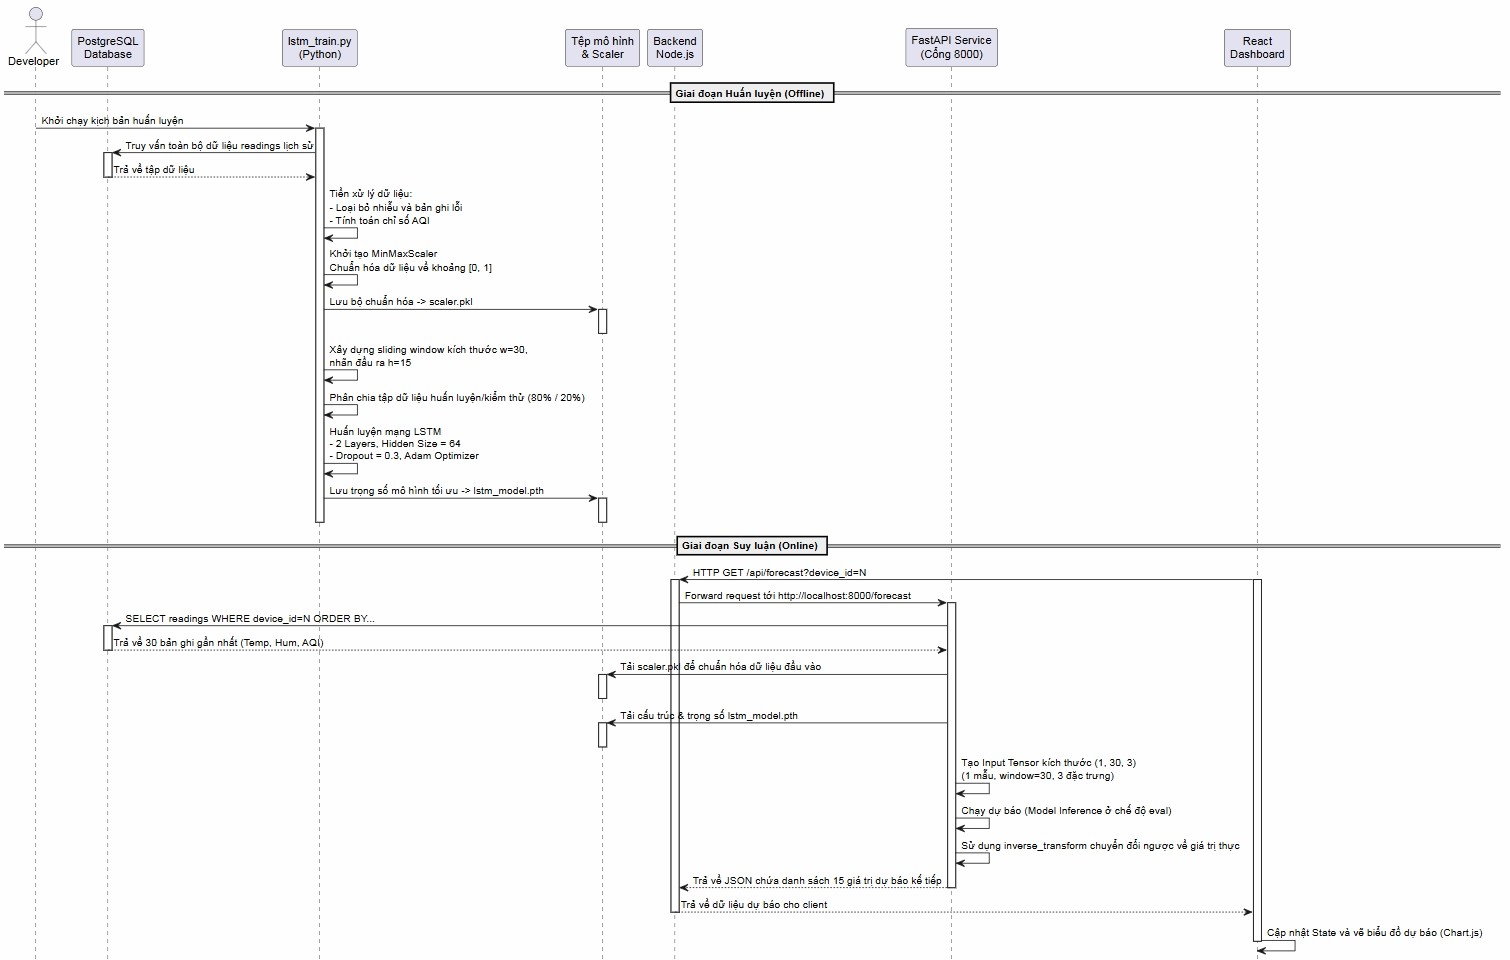
\includegraphics[width=0.9\textwidth]{lstm_pipeline}
  \caption{Pipeline dự báo chuỗi thời gian LSTM qua FastAPI microservice}
  \label{fig:lstm_pipeline}
\end{figure}

Đồ án triển khai \textbf{hai mô hình LSTM song song}:
\texttt{lstm\_model.pth} dự báo ngắn hạn 15 phút và
\texttt{lstm\_model\_long.pth} dự báo dài hạn hơn, mỗi mô hình có
scaler riêng (\texttt{scaler.pkl} và \texttt{scaler\_long.pkl}). Người
dùng có thể chọn chế độ dự báo phù hợp từ dashboard.

\subsection{Kết quả đạt được}
\label{subsec:contrib:lstm:result}

Giải pháp FastAPI microservice mang lại các kết quả cụ thể:

\begin{itemize}[leftmargin=2cm]
  \item \textbf{Tách biệt hoàn toàn:} Backend Node.js không bị block
    trong quá trình inference. Khi FastAPI service gặp sự cố, backend
    trả về lỗi graceful thay vì crash toàn hệ thống.
  \item \textbf{Thời gian inference:} Mỗi lần dự báo 15 phút cho một
    node hoàn thành trong dưới 200ms trên môi trường CPU (không GPU),
    đáp ứng yêu cầu realtime của hệ thống.
  \item \textbf{Mô hình hội tụ tốt:} Loss curve
    (Hình~\ref{fig:lstm_loss_curve}) cho thấy training loss và
    validation loss giảm đều trong quá trình huấn luyện. Kết quả hiện
    tại được sử dụng làm mốc đánh giá ban đầu và có thể tiếp tục cải
    thiện khi mở rộng tập dữ liệu hoặc tinh chỉnh siêu tham số.
  \item \textbf{Khả năng mở rộng:} Việc thay thế kiến trúc mô hình
    chỉ cần sửa file Python trong FastAPI service mà không cần thay
    đổi bất kỳ dòng code nào trong Node.js.
\end{itemize}

\subsection{Đánh giá độ chính xác mô hình}
\label{subsec:contrib:lstm:evaluation}

Độ chính xác của mô hình được đánh giá bằng sai số tuyệt đối trung
bình (Mean Absolute Error - MAE) tại ba mốc dự báo 6 phút, 10 phút và
15 phút. Các chỉ số trong Bảng~\ref{tab:lstm_mae_by_horizon} là kết
quả thực nghiệm hiện tại, được dùng làm baseline ban đầu cho hệ thống.
Trong các lần huấn luyện tiếp theo, kết quả này có thể tiếp tục được
cải thiện bằng cách bổ sung dữ liệu huấn luyện, điều chỉnh kích thước
window, số tầng LSTM hoặc các siêu tham số tối ưu hóa.

\begin{figure}[H]
  \centering
  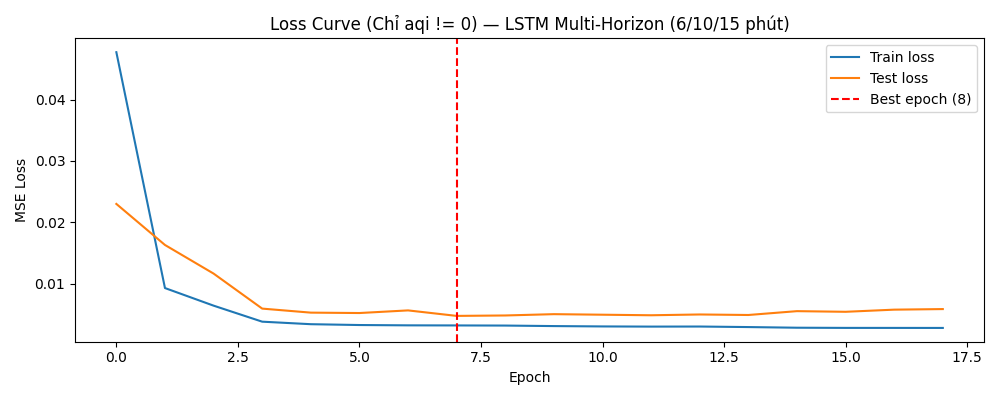
\includegraphics[width=0.82\textwidth]{loss_curve}
  \caption{Đường cong loss trong quá trình huấn luyện mô hình LSTM}
  \label{fig:lstm_loss_curve}
\end{figure}

\begin{table}[H]
  \centering
  \caption{Sai số MAE của mô hình LSTM theo từng mốc dự báo}
  \label{tab:lstm_mae_by_horizon}
  \begin{tabular}{lccc}
    \toprule
    \textbf{Mốc dự báo} & \textbf{MAE nhiệt độ ($^\circ$C)}
      & \textbf{MAE độ ẩm (\%)} & \textbf{MAE AQI} \\
    \midrule
    6 phút  & 0.216 & 0.910 & 4.854 \\
    10 phút & 0.244 & 0.880 & 4.921 \\
    15 phút & 0.278 & 0.921 & 5.012 \\
    \bottomrule
  \end{tabular}
\end{table}

Kết quả cho thấy sai số nhiệt độ duy trì dưới 0.3$^\circ$C ở cả ba
mốc dự báo, trong khi sai số độ ẩm xấp xỉ 1\%. Sai số AQI dao động
trong khoảng 4.854 đến 5.012, phù hợp cho mục tiêu cảnh báo xu hướng
và hỗ trợ người dùng ra quyết định sớm. Khi horizon tăng từ 6 phút lên
15 phút, MAE nhiệt độ và AQI tăng nhẹ, phản ánh đặc trưng thường gặp
của bài toán dự báo chuỗi thời gian: mốc dự báo càng xa thì độ bất
định càng lớn.

%------------------------------------------------------------
\section{Nội suy không gian Kriging/IDW để tạo heatmap phân bố
môi trường}
\label{sec:contrib:spatial}
%------------------------------------------------------------

\subsection{Đặt vấn đề}
\label{subsec:contrib:spatial:problem}

Với $n$ node cảm biến đặt rải rác trong không gian phòng, hệ thống chỉ
có $n$ điểm dữ liệu rời rạc tại $n$ vị trí cố định. Người vận hành
muốn biết điều kiện môi trường tại \textbf{bất kỳ điểm nào} trong
phòng, không chỉ tại vị trí đặt cảm biến. Các thách thức cụ thể:

\begin{itemize}[leftmargin=2cm]
  \item \textbf{Số lượng node hạn chế:} Trong môi trường thực tế,
    không thể đặt cảm biến dày đặc khắp nơi do chi phí và hạ tầng.
    Với ít node, nội suy biên (vùng góc phòng xa tất cả node) thường
    cho kết quả kém chính xác.
  \item \textbf{Phân bố không đều:} Các node thường tập trung ở một
    số vị trí thuận tiện, không phân bố đều trong không gian, gây ra
    hiệu ứng clustering làm méo kết quả nội suy.
  \item \textbf{Hiệu năng realtime:} Tính toán nội suy trên lưới
    40$\times$50 = 2000 điểm phải đủ nhanh để dashboard cập nhật
    trong vài giây.
\end{itemize}

\subsection{Giải pháp}
\label{subsec:contrib:spatial:solution}

Hệ thống triển khai chiến lược nội suy hai tầng kết hợp
\textbf{IDW để sinh node ảo} và \textbf{Kriging để nội suy chính}.

\textbf{Tầng 1 - Sinh node ảo bằng IDW:}

Để cải thiện độ bao phủ tại các góc phòng, trước khi chạy Kriging,
hệ thống dùng IDW để sinh thêm các \textbf{node ảo (virtual nodes)}
tại các góc và cạnh phòng. Giá trị của node ảo được ước tính từ các
node thực theo công thức IDW:

\begin{equation}
  \hat{z}_{corner} = \frac{\displaystyle\sum_{i=1}^{n}
    \frac{z_i}{d_i^2}}
    {\displaystyle\sum_{i=1}^{n} \frac{1}{d_i^2}}
\end{equation}

Trong đó $d_i$ là khoảng cách từ góc phòng đến node thực $i$, và
$z_i$ là giá trị nhiệt độ, độ ẩm hoặc AQI của node $i$. Các node ảo này
được thêm vào tập điểm đầu vào cho Kriging, giúp thuật toán có thêm
thông tin ở vùng biên, tránh hiện tượng extrapolation không kiểm soát.

\textbf{Tầng 2 - Nội suy Kriging trên toàn bộ lưới:}

Mã giả của quy trình nội suy không gian được trình bày dưới đây:

\begin{lstlisting}[language=Python, caption={Spatial interpolation pseudocode (Kriging/IDW)}, label={lst:spatial}]
from pykrige.ok import OrdinaryKriging
from scipy.interpolate import griddata
import numpy as np

def spatial_forecast(nodes: list[dict], room: dict):
    """
    nodes: [{"lat": ..., "lng": ...,
              "temperature": ..., "humidity": ..., "aqi": ...}, ...]
    room:  {"center_lat", "center_lng",
             "width_m", "length_m"}
    """
    # 1. Create virtual nodes at 4 room corners via IDW
    corners = get_room_corners(room)
    virtual_nodes = [idw_estimate(c, nodes)
                     for c in corners]
    all_nodes = nodes + virtual_nodes

    # 2. Extract coordinates and values
    lats = [n["lat"] for n in all_nodes]
    lngs = [n["lng"] for n in all_nodes]
    temps = [n["temperature"] for n in all_nodes]
    hums  = [n["humidity"]    for n in all_nodes]

    # 3. Create 40x50 target grid
    grid_lat = np.linspace(min(lats), max(lats), 40)
    grid_lng = np.linspace(min(lngs), max(lngs), 50)
    grid_lat2d, grid_lng2d = np.meshgrid(
        grid_lat, grid_lng, indexing='ij')

    # 4. Kriging interpolation for temperature
    ok_temp = OrdinaryKriging(
        lngs, lats, temps,
        variogram_model='gaussian',
        verbose=False, enable_plotting=False)
    z_temp, _ = ok_temp.execute(
        'grid', grid_lng, grid_lat)

    # 5. Kriging interpolation for humidity
    ok_hum = OrdinaryKriging(
        lngs, lats, hums,
        variogram_model='gaussian',
        verbose=False, enable_plotting=False)
    z_hum, _ = ok_hum.execute(
        'grid', grid_lng, grid_lat)

    return {
        "grid_lat": grid_lat.tolist(),
        "grid_lng": grid_lng.tolist(),
        "temperature_grid": z_temp.tolist(),
        "humidity_grid":    z_hum.tolist()
    }
\end{lstlisting}

Kết quả lưới 40$\times$50 điểm được gửi về frontend dưới dạng JSON.
Dashboard React dùng \textbf{react-leaflet} để render lưới này thành
lớp heatmap màu sắc (gradient từ xanh lam đến đỏ) phủ lên bản đồ sàn
phòng cho từng chỉ số nhiệt độ, độ ẩm hoặc AQI, như minh họa trong Hình~\ref{fig:heatmap_demo}.

\begin{figure}[H]
  \centering
  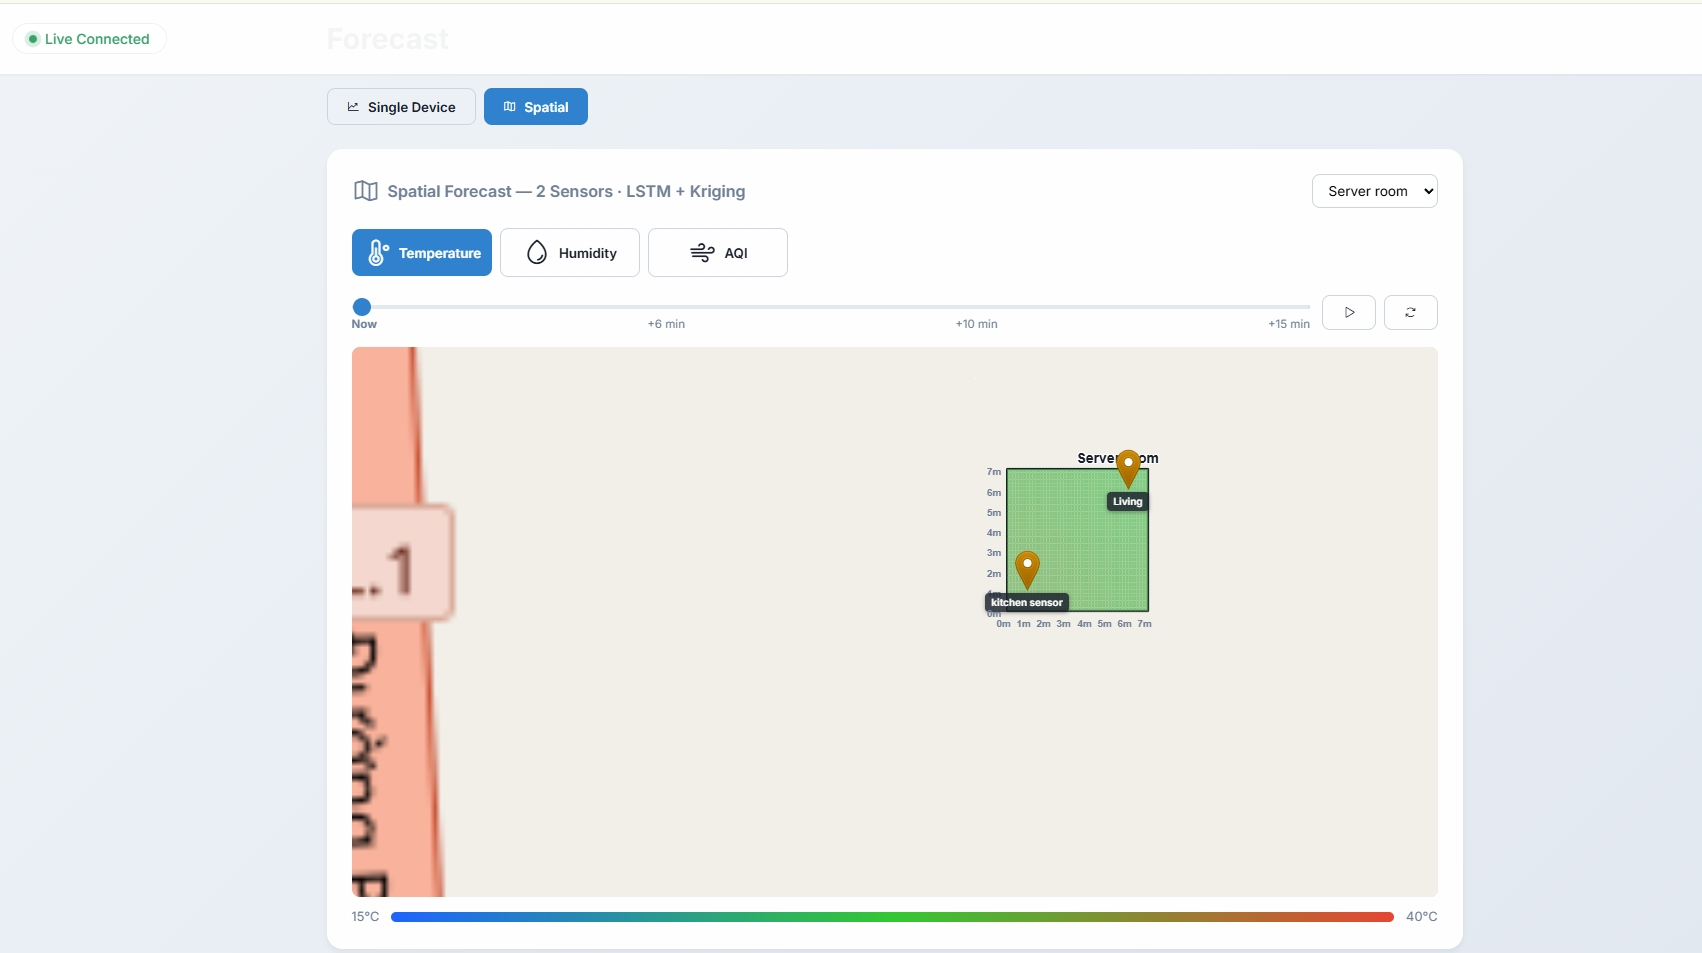
\includegraphics[width=0.9\textwidth]{system_spatial_forecast}
  \caption{Heatmap phân bố môi trường không gian được tạo từ nội suy Kriging, hiển thị trên bản đồ Leaflet}
  \label{fig:heatmap_demo}
\end{figure}

\subsection{Kết quả đạt được}
\label{subsec:contrib:spatial:result}

\begin{itemize}[leftmargin=2cm]
  \item \textbf{Bao phủ toàn không gian:} Từ $n$ điểm đo rời rạc, hệ
    thống tái tạo bản đồ phân bố liên tục trên toàn bộ diện tích
    phòng với độ phân giải lưới 40$\times$50 điểm.
  \item \textbf{Node ảo cải thiện biên:} Kỹ thuật sinh node ảo tại
    góc phòng bằng IDW giúp Kriging cho kết quả mượt mà hơn ở vùng
    biên, tránh hiệu ứng extrapolation bất thường khi không có node
    thực tại vùng đó.
  \item \textbf{Hiệu năng đủ dùng:} Thời gian tính toán Kriging cho
    lưới 40$\times$50 trên CPU thông thường dưới 2 giây, đáp ứng yêu
    cầu cập nhật heatmap theo yêu cầu của người dùng.
  \item \textbf{Kết hợp dự báo:} Heatmap có thể được tạo không chỉ
    từ dữ liệu thực đo hiện tại mà còn từ kết quả dự báo LSTM, cho
    phép người dùng xem \textbf{heatmap dự báo} - phân bố môi
    trường ước tính trong 15 phút tới.
\end{itemize}

%------------------------------------------------------------
\section{Kiến trúc truyền thông MQTT kết hợp Socket.io đảm bảo
độ trễ thấp}
\label{sec:contrib:comm}
%------------------------------------------------------------

\subsection{Đặt vấn đề}
\label{subsec:contrib:comm:problem}

Hệ thống quan trắc realtime đặt ra yêu cầu nghiêm ngặt về độ trễ
end-to-end: từ khi cảm biến đọc giá trị đến khi biểu đồ trên dashboard
được cập nhật phải dưới 2 giây. Cách tiếp cận đơn giản nhất là
\textbf{HTTP polling} - frontend định kỳ gọi API để lấy dữ liệu mới
- nhưng có nhiều nhược điểm:

\begin{itemize}[leftmargin=2cm]
  \item \textbf{Độ trễ không xác định:} Nếu polling mỗi 5 giây, độ
    trễ trung bình là 2.5 giây, tệ nhất là 5 giây.
  \item \textbf{Lãng phí tài nguyên:} Hầu hết các request polling
    trả về ``không có dữ liệu mới'', tốn băng thông và CPU server
    vô ích.
  \item \textbf{Không scalable:} Với 100 client đang mở dashboard,
    server nhận 20 request/giây chỉ để kiểm tra dữ liệu mới.
\end{itemize}

Ngoài ra, giao tiếp giữa node IoT và server cũng cần được thiết kế
cẩn thận: HTTP POST từ ESP32 mỗi 5 giây tạo ra overhead lớn (TCP
handshake, HTTP headers ~500 bytes) cho thiết bị có tài nguyên hạn chế.

\subsection{Giải pháp}
\label{subsec:contrib:comm:solution}

Hệ thống áp dụng chiến lược \textbf{hai giao thức bổ trợ nhau}: MQTT
cho luồng dữ liệu từ node IoT lên server, và Socket.io cho luồng dữ
liệu từ server xuống dashboard.

\textbf{Tầng 1 - MQTT (Node IoT $\to$ Server):}

MQTT được chọn vì overhead tối thiểu: header chỉ 2 byte cố định, kết
nối TCP được duy trì liên tục (persistent connection) nên không tốn
chi phí handshake mỗi lần gửi. Mỗi 5 giây, ESP32 publish một message
nhỏ gọn:

\begin{lstlisting}[language=C, caption={MQTT payload from ESP32 node},
label={lst:mqtt_payload}]
// JSON payload sent via MQTT: ~60 bytes
StaticJsonDocument<128> doc;
doc["temperature"] = temperature;
doc["humidity"]    = humidity;
doc["aqi"]         = aqi; // bat buoc cho ML pipeline

char payload[128];
serializeJson(doc, payload);

// Publish to topic device/{api_key}/data
client.publish(topic.c_str(), payload.c_str());
\end{lstlisting}

\textbf{Tầng 2 - Aedes Broker (Server-side MQTT):}

Thay vì triển khai Mosquitto broker riêng biệt, hệ thống tích hợp
\textbf{Aedes} - MQTT broker thuần Node.js - trực tiếp trong tiến
trình backend. Điều này cho phép xử lý message MQTT trong cùng event
loop với logic nghiệp vụ, tránh độ trễ mạng giữa broker và backend:

\begin{lstlisting}[language=JavaScript, caption={MQTT message handling
in Aedes broker}, label={lst:aedes}]
aedes.on('publish', async (packet, client) => {
  const topic = packet.topic;

  // Only handle sensor data topics
  if (!topic.startsWith('device/')) return;

  // 1. Extract api_key from topic
  const apiKey = topic.split('/')[1];

  // 2. Validate and get device_id from PostgreSQL
  const device = await db.query(
    'SELECT id, owner_user_id FROM devices
     WHERE api_key=$1', [apiKey]);
  if (!device.rows.length) return;  // skip if invalid key

  // 3. Parse JSON payload
  const { temperature, humidity, aqi } = JSON.parse(
    packet.payload.toString());

  // 4. Save to PostgreSQL
  await db.query(
    'INSERT INTO readings
     (device_id, temperature, humidity, aqi, timestamp)
     VALUES ($1,$2,$3,$4,NOW())',
    [device.rows[0].id, temperature, humidity, aqi]);

  // 5. Check alert thresholds (alertService)
  await alertService.check(device.rows[0], {
    temperature, humidity, aqi });

  // 6. Push realtime to dashboard via Socket.io
  io.to(`device_${device.rows[0].id}`)
    .emit('new_reading', { temperature, humidity, aqi,
                           timestamp: new Date() });
});
\end{lstlisting}

\textbf{Tầng 3 - Socket.io (Server $\to$ Dashboard):}

Khi dashboard mở, client xác thực bằng JWT và đăng ký nhận dữ liệu
của thiết bị cụ thể:

\begin{lstlisting}[language=JavaScript, caption={Client-side Socket.io in React dashboard}, label={lst:socketio_client}]
// Connect and authenticate
const socket = io(SERVER_URL);
socket.emit('authenticate', { token: jwtToken });

// Subscribe to device data
socket.emit('subscribe_device', { deviceId });

// Listen for new data and update chart
socket.on('new_reading', (data) => {
  setChartData(prev => ({
    labels: [...prev.labels, data.timestamp],
    temperature: [...prev.temperature, data.temperature],
    humidity:    [...prev.humidity,    data.humidity],
    aqi:         [...prev.aqi,         data.aqi]
  }));
});
\end{lstlisting}

Hình~\ref{fig:comm_flow} minh họa toàn bộ luồng truyền thông từ node
ESP32 đến dashboard với các mốc thời gian tương ứng.

\begin{figure}[H]
  \centering
  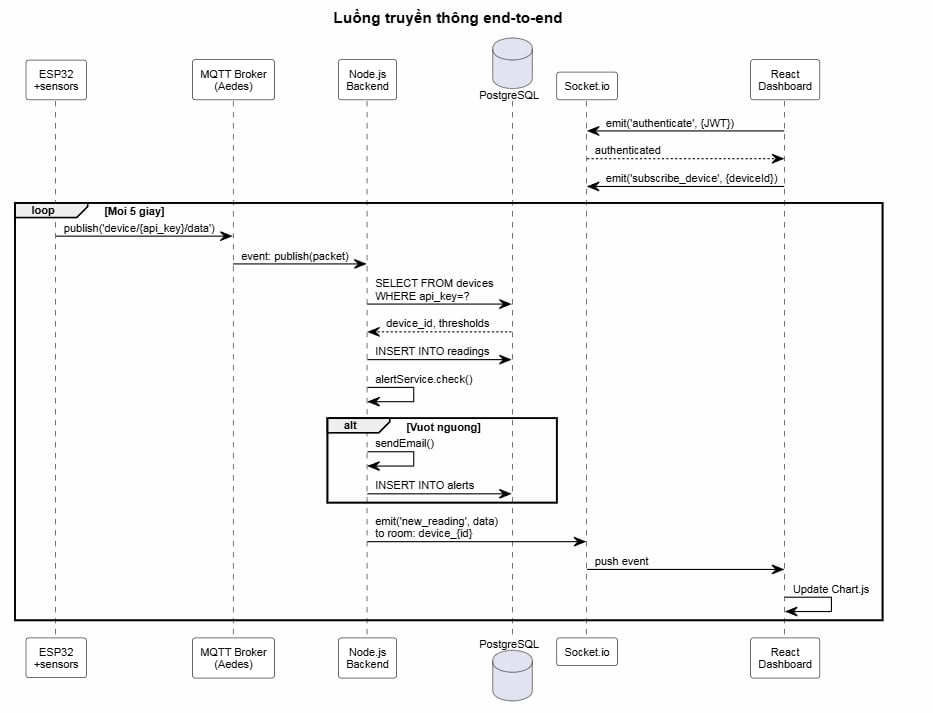
\includegraphics[width=0.9\textwidth]{comm_flow}
  \caption{Luồng truyền thông end-to-end của hệ thống}
  \label{fig:comm_flow}
\end{figure}

\subsection{Kết quả đạt được}
\label{subsec:contrib:comm:result}

\begin{itemize}[leftmargin=2cm]
  \item \textbf{Độ trễ end-to-end thấp:} Từ khi ESP32 publish message
    MQTT đến khi biểu đồ Chart.js trên dashboard cập nhật, độ trễ
    trung bình đo được dưới 500ms trong điều kiện mạng LAN, đáp ứng
    tốt yêu cầu realtime.
  \item \textbf{Không polling:} Socket.io push-based hoàn toàn loại bỏ
    HTTP polling, giảm số lượng request xuống backend từ $O(n_{client}
    \times f_{poll})$ về 0 khi không có dữ liệu mới.
  \item \textbf{Aedes tích hợp đơn giản hóa triển khai:} Không cần
    cài đặt và vận hành Mosquitto riêng biệt. Toàn bộ hệ thống backend
    chỉ cần một tiến trình Node.js duy nhất với lệnh \texttt{node
    server/index.js}.
  \item \textbf{Xác thực hai lớp:} Node IoT xác thực bằng
    \texttt{api\_key} qua MQTT, người dùng dashboard xác thực bằng JWT
    qua Socket.io. Hai lớp xác thực độc lập đảm bảo chỉ thiết bị hợp
    lệ mới được ghi dữ liệu và chỉ người dùng hợp lệ mới xem được.
  \item \textbf{Phòng Socket.io theo device/user:} Server emit đến room
    \texttt{device\_\{id\}} và \texttt{user\_\{id\}}, đảm bảo mỗi
    client chỉ nhận dữ liệu của thiết bị mình đang xem, không bị
    ``nhiễu'' từ các thiết bị khác.
\end{itemize}


% TÀI LIỆU THAM KHẢO
\clearpage
\bibliographystyle{IEEEtran}
\bibliography{references}
\addcontentsline{toc}{chapter}{TÀI LIỆU THAM KHẢO}

% PHỤ LỤC
\clearpage
\appendix
%============================================================
% PHỤ LỤC: MÃ NGUỒN QUAN TRỌNG
%============================================================
\chapter{PHỤ LỤC: MÃ NGUỒN QUAN TRỌNG}
\label{chap:appendix}

Phần phụ lục này lưu trữ mã nguồn chi tiết của các thành phần cốt lõi trong hệ thống AIoT giám sát và dự báo chất lượng không khí, phục vụ mục đích tham khảo kỹ thuật.

\section{Mã nguồn Firmware ESP32}

\begin{lstlisting}[language=C, caption={Luồng xử lý chính của Firmware ESP32}, label={lst:firmware_main}]
// sensor/sensor.ino (Luoc trich phan vong lap chinh)
#include <WiFi.h>
#include <PubSubClient.h>
#include <ArduinoJson.h>
#include <DHT.h>
#include <Preferences.h>
#include <WiFiManager.h>

#define DHTPIN 4
#define DHTTYPE DHT11
#define SEND_INTERVAL 5000   // 5 giay

DHT dht(DHTPIN, DHTTYPE);
WiFiClient wifiClient;
PubSubClient mqttClient(wifiClient);

String deviceApiKey = "";
int    deviceId     = -1;
bool   provisioned  = false;

void setup() {
    dht.begin();
    loadCredentials();  // Doc device_id, api_key tu Flash
    WiFiManager wm;
    wm.autoConnect("Sensor-Setup-[MAC]");
    mqttClient.setServer(MQTT_BROKER, 1883);
    mqttClient.setCallback(mqttCallback);
}

void loop() {
    if (!provisioned) { sendProvisionRequest(); return; }
    if (!mqttClient.connected()) reconnectWithAuth();
    mqttClient.loop();

    // Gui du lieu theo chu ky SEND_INTERVAL
    if (millis() - lastSend >= SEND_INTERVAL) {
        float temp = dht.readTemperature();
        float hum  = dht.readHumidity();
        float aqi  = generateMockAqi(); // Gia lap AQI

        if (!isnan(temp) && !isnan(hum)) {
            publishData(temp, hum, aqi);
        }
        lastSend = millis();
    }
}

void publishData(float temp, float hum, float aqi) {
    StaticJsonDocument<128> doc;
    doc["temperature"] = temp;
    doc["humidity"]    = hum;
    doc["aqi"]         = aqi;
    char payload[128];
    serializeJson(doc, payload);

    String topic = "device/" + deviceApiKey + "/data";
    mqttClient.publish(topic.c_str(), payload);
}
\end{lstlisting}

\section{Cấu trúc Cơ sở dữ liệu và Dịch vụ Cảnh báo Backend}

\begin{lstlisting}[language=SQL, caption={Schema cơ sở dữ liệu PostgreSQL}, label={lst:schema}]
-- Bang nguoi dung
CREATE TABLE users (
    id         SERIAL PRIMARY KEY,
    name       VARCHAR(100),
    email      VARCHAR(100) UNIQUE NOT NULL,
    password   VARCHAR(255) NOT NULL,    -- bcrypt hash
    role       VARCHAR(20) DEFAULT 'user',
    created_at TIMESTAMP DEFAULT NOW()
);

-- Bang phong/khu vuc
CREATE TABLE rooms (
    id            SERIAL PRIMARY KEY,
    name          VARCHAR(100),
    description   TEXT,
    center_lat    REAL,
    center_lng    REAL,
    width_m       REAL,
    length_m      REAL,
    owner_user_id INTEGER REFERENCES users(id),
    created_at    TIMESTAMP DEFAULT NOW()
);

-- Bang thiet bi IoT
CREATE TABLE devices (
    id               SERIAL PRIMARY KEY,
    name             VARCHAR(100),
    description      TEXT,
    owner_user_id    INTEGER REFERENCES users(id),
    api_key          VARCHAR(64) UNIQUE NOT NULL,
    notify_email     BOOLEAN DEFAULT TRUE,
    temp_high        REAL DEFAULT 35.0,
    temp_low         REAL DEFAULT 10.0,
    hum_high         REAL DEFAULT 80.0,
    hum_low          REAL DEFAULT 20.0,
    aqi_high         REAL,
    aqi_low          REAL,
    room_id          INTEGER REFERENCES rooms(id),
    mac_address      VARCHAR(17) UNIQUE,
    x                DOUBLE PRECISION,
    y                DOUBLE PRECISION,
    lat              DOUBLE PRECISION,
    lng              DOUBLE PRECISION,
    firmware_version VARCHAR(50),
    chip_model       VARCHAR(50),
    created_at       TIMESTAMP DEFAULT NOW()
);

-- Bang du lieu cam bien
CREATE TABLE readings (
    id          SERIAL PRIMARY KEY,
    device_id   INTEGER REFERENCES devices(id),
    temperature REAL NOT NULL,
    humidity    REAL NOT NULL,
    aqi         REAL NOT NULL DEFAULT 0,
    timestamp   TIMESTAMP DEFAULT NOW()
);

-- Index tang toc truy van chuoi thoi gian
CREATE INDEX idx_readings_device_time
    ON readings(device_id, timestamp DESC);

-- Bang canh bao
CREATE TABLE alerts (
    id              SERIAL PRIMARY KEY,
    device_id       INTEGER REFERENCES devices(id),
    type            VARCHAR(50),
    value           REAL,
    message         TEXT,
    acknowledged_by INTEGER REFERENCES users(id),
    acknowledged_at TIMESTAMP,
    timestamp       TIMESTAMP DEFAULT NOW()
);
\end{lstlisting}

\begin{lstlisting}[language=JavaScript, caption={Logic dịch vụ kiểm tra ngưỡng cảnh báo (Backend Node.js)}, label={lst:alert_service}]
// server/services/alertService.js
async function check(device, reading) {
    const { temperature, humidity } = reading;
    const alerts = [];

    if (temperature > device.temp_high)
        alerts.push({ type: 'temp_high', value: temperature,
            message: `Nhiet do ${temperature}C vuot nguong ${device.temp_high}C` });
            
    if (temperature < device.temp_low)
        alerts.push({ type: 'temp_low', value: temperature,
            message: `Nhiet do ${temperature}C duoi nguong ${device.temp_low}C` });
            
    if (humidity > device.hum_high)
        alerts.push({ type: 'hum_high', value: humidity,
            message: `Do am ${humidity}% vuot nguong ${device.hum_high}%` });
            
    if (humidity < device.hum_low)
        alerts.push({ type: 'hum_low', value: humidity,
            message: `Do am ${humidity}% duoi nguong ${device.hum_low}%` });
            
    for (const alert of alerts) {
        // Luu vao DB
        await db.query(
            `INSERT INTO alerts
             (device_id, type, value, message, timestamp)
             VALUES ($1,$2,$3,$4,NOW())`,
            [device.id, alert.type,
             alert.value, alert.message]);
             
        // Gui email neu thiet bi bat thong bao
        if (device.notify_email)
            await emailService.sendAlert(device, alert);
    }
}
\end{lstlisting}

\section{Mã nguồn Python Machine Learning Service}

\begin{lstlisting}[language=Python, caption={Quy trình huấn luyện mô hình dự báo LSTM}, label={lst:lstm_train}]
# lstm_train/train.py (Trich doan quy trinh)
import torch
import torch.nn as nn
from sklearn.preprocessing import MinMaxScaler
import joblib

# 1. Load data from PostgreSQL
data = query("SELECT temperature, humidity, aqi FROM readings ORDER BY timestamp")

# 2. Min-Max normalization, save scaler for inference reuse
scaler = MinMaxScaler()
data_scaled = scaler.fit_transform(data)
joblib.dump(scaler, 'scaler.pkl')

# 3. Create (X, y) pairs using sliding window
X, y = create_sequences(data_scaled, window=30, horizon=15)

# 4. Define LSTM architecture (PyTorch)
class LSTMModel(nn.Module):
    def __init__(self):
        super().__init__()
        self.lstm = nn.LSTM(input_size=3,
                            hidden_size=64,
                            num_layers=2,
                            batch_first=True,
                            dropout=0.3)  # Da cap nhat dropout=0.3
        self.fc = nn.Linear(64, 15 * 3)

    def forward(self, x):
        out, _ = self.lstm(x)
        return self.fc(out[:, -1, :]).view(-1, 15, 3)

# 5. Train with Adam optimizer, MSE loss
model = LSTMModel()
optimizer = torch.optim.Adam(model.parameters(), lr=1e-3)
criterion = nn.MSELoss()

for epoch in range(num_epochs):
    pred = model(X_train)
    loss = criterion(pred, y_train)
    optimizer.zero_grad()
    loss.backward()
    optimizer.step()

# 6. Save model weights
torch.save(model.state_dict(), 'lstm_model.pth')
\end{lstlisting}

\begin{lstlisting}[language=Python, caption={Phục vụ suy luận mô hình LSTM qua FastAPI Service}, label={lst:lstm_infer}]
# forecast/time_forecast/main.py (Phan API inference)
from fastapi import FastAPI, Depends
import torch
import joblib

model = LSTMModel()
model.load_state_dict(torch.load('lstm_model.pth'))
model.eval()
scaler = joblib.load('scaler.pkl')

@app.get("/forecast")
async def forecast(device_id: int, db=Depends(get_db)):
    # 1. Fetch 30 latest records from PostgreSQL
    rows = await db.fetch(
        "SELECT temperature, humidity, aqi FROM readings WHERE device_id=$1 ORDER BY timestamp DESC LIMIT 30", device_id)

    # 2. Normalize using saved scaler
    data = scaler.transform(rows)

    # 3. Create input tensor
    X = torch.tensor(data).unsqueeze(0).float()

    # 4. Inference (no_grad to save memory)
    with torch.no_grad():
        pred = model(X)

    # 5. Inverse transform to real values
    result = scaler.inverse_transform(pred.squeeze(0).numpy())

    return {"forecast": result.tolist()}
\end{lstlisting}

\begin{lstlisting}[language=Python, caption={Thuật toán nội suy không gian địa thống kê Kriging/IDW}, label={lst:spatial}]
# forecast/spatial_forecast.py
from pykrige.ok import OrdinaryKriging
import numpy as np

def spatial_forecast(nodes: list[dict], room: dict):
    # 1. Create virtual nodes at 4 room corners via IDW
    corners = get_room_corners(room)
    virtual_nodes = [idw_estimate(c, nodes) for c in corners]
    all_nodes = nodes + virtual_nodes

    # 2. Extract coordinates and values
    lats = [n["lat"] for n in all_nodes]
    lngs = [n["lng"] for n in all_nodes]
    temps = [n["temperature"] for n in all_nodes]
    hums  = [n["humidity"]    for n in all_nodes]

    # 3. Create 40x50 target grid
    grid_lat = np.linspace(min(lats), max(lats), 40)
    grid_lng = np.linspace(min(lngs), max(lngs), 50)

    # 4. Kriging interpolation for temperature
    ok_temp = OrdinaryKriging(
        lngs, lats, temps,
        variogram_model='gaussian',
        verbose=False, enable_plotting=False)
    z_temp, _ = ok_temp.execute('grid', grid_lng, grid_lat)

    # 5. Kriging interpolation for humidity
    ok_hum = OrdinaryKriging(
        lngs, lats, hums,
        variogram_model='gaussian',
        verbose=False, enable_plotting=False)
    z_hum, _ = ok_hum.execute('grid', grid_lng, grid_lat)

    return {
        "grid_lat": grid_lat.tolist(),
        "grid_lng": grid_lng.tolist(),
        "temperature_grid": z_temp.tolist(),
        "humidity_grid":    z_hum.tolist()
    }
\end{lstlisting}


\end{document}
